\documentclass[11pt]{aghdpl}
% \documentclass[en,11pt]{aghdpl}  % praca w języku angielskim

% Lista wszystkich języków stanowiących języki pozycji bibliograficznych użytych w pracy.
% (Zgodnie z zasadami tworzenia bibliografii każda pozycja powinna zostać utworzona zgodnie z zasadami języka, w którym dana publikacja została napisana.)
\usepackage[english,polish]{babel}

% Użyj polskiego łamania wyrazów (zamiast domyślnego angielskiego).
\usepackage{polski}

\usepackage[utf8]{inputenc}

% dodatkowe pakiety

\usepackage{mathtools}
\usepackage{amsfonts}
\usepackage{amsmath}
\usepackage{amsthm}

% --- < bibliografia > ---

\usepackage[
style=numeric,
sorting=none,
%
% Zastosuj styl wpisu bibliograficznego właściwy językowi publikacji.
language=autobib,
autolang=other,
% Zapisuj datę dostępu do strony WWW w formacie RRRR-MM-DD.
urldate=iso8601,
% Nie dodawaj numerów stron, na których występuje cytowanie.
backref=false,
% Podawaj ISBN.
isbn=true,
% Nie podawaj URL-i, o ile nie jest to konieczne.
url=false,
%
% Ustawienia związane z polskimi normami dla bibliografii.
maxbibnames=3,
% Jeżeli używamy BibTeXa:
backend=bibtex
]{biblatex}

\usepackage{csquotes}
% Ponieważ `csquotes` nie posiada polskiego stylu, można skorzystać z mocno zbliżonego stylu chorwackiego.
\DeclareQuoteAlias{croatian}{polish}

\addbibresource{bibliografia.bib}

% Nie wyświetlaj wybranych pól.
%\AtEveryBibitem{\clearfield{note}}


% ------------------------
% --- < listingi > ---

% Użyj czcionki kroju Courier.
\usepackage{courier}

\usepackage{listings}
\lstloadlanguages{TeX}

\lstset{
	literate={ą}{{\k{a}}}1
           {ć}{{\'c}}1
           {ę}{{\k{e}}}1
           {ó}{{\'o}}1
           {ń}{{\'n}}1
           {ł}{{\l{}}}1
           {ś}{{\'s}}1
           {ź}{{\'z}}1
           {ż}{{\.z}}1
           {Ą}{{\k{A}}}1
           {Ć}{{\'C}}1
           {Ę}{{\k{E}}}1
           {Ó}{{\'O}}1
           {Ń}{{\'N}}1
           {Ł}{{\L{}}}1
           {Ś}{{\'S}}1
           {Ź}{{\'Z}}1
           {Ż}{{\.Z}}1,
	basicstyle=\footnotesize\ttfamily,
}

% ------------------------

\AtBeginDocument{
	\renewcommand{\tablename}{Tabela}
	\renewcommand{\figurename}{Rys.}
}

% ------------------------
% --- < tabele > ---

\usepackage{array}
\usepackage{tabularx}
\usepackage{multirow}
\usepackage{booktabs}
\usepackage{makecell}
\usepackage[flushleft]{threeparttable}

% defines the X column to use m (\parbox[c]) instead of p (`parbox[t]`)
\newcolumntype{C}[1]{>{\hsize=#1\hsize\centering\arraybackslash}X}


%---------------------------------------------------------------------------

\author{Paweł Milota, Jan Posz}
\shortauthor{P. Milota, J. Posz}

%\titlePL{Przygotowanie bardzo długiej i pasjonującej pracy dyplomowej w~systemie~\LaTeX}
%\titleEN{Preparation of a very long and fascinating bachelor or master thesis in \LaTeX}

\titlePL{Opracowanie algorytmu wyszukiwania tras dla rowerzystów na podstawie heterogenicznych zbiorów danych geo-przestrzennych}
\titleEN{Development of the search algorithm of routes for cyclists on the basis of heterogeneous geo-spatial data sets.}


\shorttitlePL{Opracowanie algorytmu wyszukiwania tras dla rowerzystów na podstawie heterogenicznych zbiorów danych geo-przestrzennych} 
\shorttitleEN{Development of the search algorithm of routes for cyclists on the basis of heterogeneous geo-spatial data sets.}

\thesistype{Praca dyplomowa magisterska}

\supervisor{dr hab. inż Mikołaj Leszczuk}
%\supervisor{Marcin Szpyrka PhD, DSc}

\degreeprogramme{Elektronika i Telekomunikacja}
%\degreeprogramme{Computer Science}

\date{2019}

\department{Katedra Telekomunikacji}

\faculty{Wydział Informatyki, Elektroniki i TElekomunikacji}

\acknowledgements{Serdecznie dziękujemy dr hab. Mikołajowi Leszczukowi za nadzór i pomoc podczas tworzenia pracy.}


\setlength{\cftsecnumwidth}{10mm}

%---------------------------------------------------------------------------
\setcounter{secnumdepth}{4}
\brokenpenalty=10000\relax

\begin{document}

\titlepages

% Ponowne zdefiniowanie stylu `plain`, aby usunąć numer strony z pierwszej strony spisu treści i poszczególnych rozdziałów.
\fancypagestyle{plain}
{
	% Usuń nagłówek i stopkę
	\fancyhf{}
	% Usuń linie.
	\renewcommand{\headrulewidth}{0pt}
	\renewcommand{\footrulewidth}{0pt}
}

\setcounter{tocdepth}{2}
\tableofcontents
\clearpage

\chapter{Cel Pracy}
\label{cha:cel_pracy}
\chapter{Wstęp}
\label{cha:wstep}
Świat się zmienia. I jak jeszcze do niedawna ogólnie rozumiany postęp był postrzegany przez pryzmat nowinek technicznych ułatwiających – w mniejszym bądź większym stopniu – codzienne czynności, tak od pewnego czasu niezwykle ważną kwestią stała się ekologia. Wkrada się ona do niemal każdego aspektu naszego życia: od naklejek na sprzęcie AGD informującym o efektywności energetycznej danego urządzenia, przez powszechne i coraz bardziej rygorystyczne normy emisji silników spalinowych, po ograniczenia w spalaniu opału w prywatnych piecach. Fala „pro eko” nabiera mocy z każdym rokiem, co jest jak najbardziej zrozumiałe w kontekście zmian do jakich dochodzi na Ziemi z powodu działalności energetycznej człowieka. Jednym z ogromnej liczby postulatów ruchu proekologicznego jest ograniczenie ruchu samochodowego, zwłaszcza tego na krótki dystans. Co więc w zamian? Odpowiedź jest prosta: niemal w stu procentach ekologiczny rower. Ten wymaga jednak odpowiedniej infrastruktury oraz nieco zmiany w podejściu do kwestii transportu. \newline
Jednak trend ten jest widoczny już do dłuższego czasu: rower coraz częściej jest wybierany jako środek transportu. Co oczywiste w większości przypadków na niedługich trasach wewnątrz miejskich, jak przejazd do i z miejsca pracy lub sklepu. Wyraźnie to widać na wykresie natężenia ruchu rowerowego (Rys. 2.1.)  na jednym z głównych węzłów komunikacyjnych Krakowa (również pod względem rowerowym), czyli na Rondzie Mogilskim. Otóż wg danych Urzędu Miasta Krakowa największą liczbę rowerzystów można zaobserwować w godzinach szczytu, co jasno pokazuje, że są to w dużej mierze ludzie dojeżdżający do i z pracy.
\begin{figure}[H]
\centering
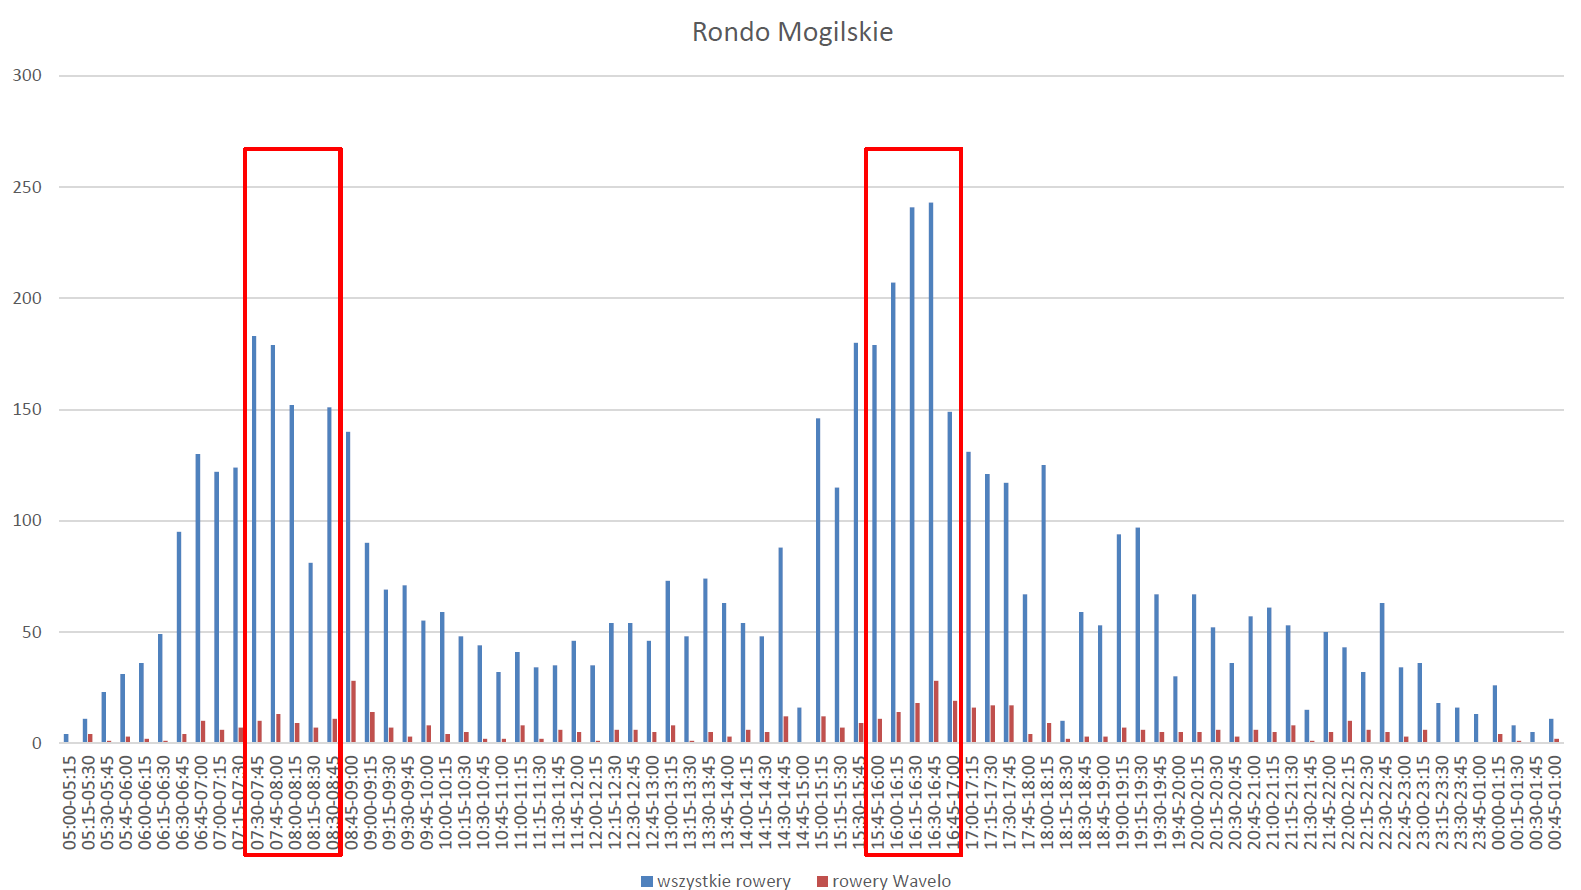
\includegraphics[width=\textwidth]{nat_ruchu_row}
\caption{[1]Natężenie ruchu rowerowego na Rondzie Mogilskim wg. Urzędu Miasta Krakowa (pomiar dokonany dnia 19.06.2018).}
\end{figure}
U podstaw niniejszego zjawiska leżą zróżnicowane przyczyny i nie wszystkie można wytłumaczyć powszechną modą na ekologię czy rosnącą popularnością roweru jako ogólnej formy rekreacji. Ważne aspekty, wpływające na wybór roweru jako środka komunikacji, to między innymi także takie kwestie jak możliwość bezproblemowego (w większości przypadków) dojazdu dokładnie do naszej destynacji, ekonomiczność takiego rodzaju komunikacji (jazda jest darmowa, jedynym wydatkiem jest kupno samego roweru), a w nierzadkich przypadkach i czasu (rower nie stoi w korkach, a jednocześnie jest dużo szybszy niż poruszanie się pieszo), czy korzyści zdrowotne wynikające z regularnego wysiłku fizycznego. Niemałym atutem roweru jest również jego łatwiejsze zaparkowanie – w centrach większych miast stojaki rowerowe są rozmieszczone całkiem gęsto i w zasadzie nigdy nie brakuje na nich miejsca, czego nie można powiedzieć o stanowiskach parkingowych dla samochodów. Te, oraz wiele innych przyczyn, pozwala zrozumieć dlaczego liczba amatorów bezsilnikowych jednośladów regularnie rośnie i nie wygląda na to by rosnąć miała przestać. Co istotniejsze nie tylko tych jeżdżących dla przyjemności w swoim czasie wolnym, ale także – a może przede wszystkim – tych korzystających z roweru jako zamiennika samochodu lub komunikacji zbiorowej. Tendencję tę można zauważyć zwłaszcza w miastach o bardzo dużym natężeniu ruchu samochodowego, co ułatwia wydedukowanie oczywistych zależności: w miastach odległości są względnie niewielkie, a powstające na głównych ciągach komunikacyjnych zatory w ruchu pojazdów mechanicznych, powodują znaczne wydłużenie czasu podróży przy użyciu tychże. Stąd rower całkiem często okazuje się wybawieniem, środkiem transportu, który zaoszczędza niemało czasu i niejako przy okazji daje okazję do poruszania się i spalenia palu kalorii. Dlatego też widok dużej ilości stojaków rowerowych ustawionych przy siedzibach największych firm nikogo nie dziwi. Wręcz przeciwnie – nie raz pracownicy jakiegoś przedsiębiorstwa potrafią wprost wypomnieć brak takiego udogodnienia.  
Obecna strategia każdego większego miasta – zwłaszcza europejskiego – opiera się niejako na stworzeniu jak największych możliwych udogodnień dla rowerzystów, jednocześnie starając się ograniczyć ruch samochodowy. Oba aspekty łączą się ze sobą w jedną spójną całość, a obrana przez miejskie władze ścieżka rozwoju nie jest podyktowana wyłącznie ekologią, ale także chłodną ekonomiczną kalkulacją. Metropolia, której drogi są permanentnie zakorkowane, w dłuższej (a czasem także i w krótszej) perspektywie czasu traci finansowo. Oczywiście straty te nie są bezpośrednie, a wynikają z odpływu mieszkańców, w efekcie czego spada liczba przedsiębiorstw, a koniec końców także i turystów.  Kraków nie chciał pozostać w tyle za innymi europejskimi miastami i również od kilku lat stara się inwestować w infrastrukturę rowerową, z gorszym lub lepszym skutkiem. Wprawdzie wdrażane i planowane inwestycje we wszelkiego rodzaju ścieżki rowerowe i innego typu udogodnienia nie zaspokajają znacznie szybciej rosnących potrzeb krakowskich rowerzystów, to jednak trzeba docenić fakt ich powstawania oraz zauważyć, że sieć tras już teraz jest całkiem przyzwoita. Efektem tego podróż z dowolnego miejsca w Krakowie przy pomocy bicykla nie jest już udręką i może być w dużej mierze realizowana po specjalnie wyznaczonym obszarze. Oczywiście lata zaniedbań powodują, że nie wszystko da się poprawić od razu, więc i w stolicy Małopolski nadal znajdują się białe plamy, gdzie teoretycznie dojazd rowerem umożliwia jedynie zwykła ulica, jednak takich miejsc systematycznie ubywa. Co najistotniejsze miejskie władze mocno skupiły się na tworzeniu ścieżek w najbardziej newralgicznych obszarach, dzięki czemu większość dużych skupisk ludzkich (gdzie na co dzień mieszka i sypia sporo mieszkańców) oraz dzielnic usługowo-handlowych czy też biznesowych (gdzie owi mieszkańcy pracują lub udają się na zakupy bądź relaks) jest ze sobą nad wyraz poprawnie skomunikowana pod względem rowerowym. \newline
Daje się jednak zauważyć, iż pomimo nie najgorszej infrastruktury, wielu krakowskich rowerzystów – często być może nieświadomie – nie wykorzystuje potencjału w niej drzemiącego. Widok rowerzysty poruszającego się po zwykłej drodze, podczas gdy istnieje alternatywna, wcale nie dłuższa ścieżka wytyczona specjalnie dla tego typu transportu, nie należy do rzadkości, pomimo faktu, iż rowerzysta ma obowiązek korzystania z drogi rowerowej, gdy ta jest poprowadzona bezpośrednio przy danej jezdni. A przecież taka sytuacja nie jest komfortowa ani dla użytkownika roweru, ani kierowcy samochodu, co więcej stanowi również dużo większe zagrożenie dla bezpieczeństwa rowerzysty. Niemałe jest także grono osób niezdecydowanych, dla których hasło „dojazd do pracy rowerem” lub podobne kojarzy się bardziej z koniecznością slalomu między samochodami, wdychaniem spalin i strachem przed potrąceniem, niż z oszczędnością czasu i pieniędzy. Tego typu ludzie również nie mają pełnej wiedzy na temat tego jak wygląda infrastruktura rowerowa w Krakowie, często przekonując się o tym dopiero po pierwszych przejazdach, metodą prób i błędów. Sytuacja ta wynika oczywiście ze sporej dynamiki rozwoju udogodnień dla rowerów, o której wspomniano wcześniej.
Trafnym staje się zatem pytanie: jak w łatwy sposób doinformować ludzi? Jak zachęcić ich do korzystania z rowerów? Rozwiązaniem wydaje się stworzenie czegoś w rodzaju swoistego przewodnika po infrastrukturze rowerowej Krakowa, dlaczego więc nie pójść krok dalej i nie stworzyć pełnoprawnej nawigacji rowerowej? Nie da się ukryć, że grupą społeczną, wśród której najprościej jest rozpropagować jakiś trend lub modę, jest grupa ludzi młodych, głównie przed 35 rokiem życia. W jaki sposób stworzyć u takich ludzi zainteresowanie? Oczywiście przy pomocy zawoalowania rozwiązania w kokon nowoczesnych rozwiązań, najlepiej więc by taka nawigacja była aplikacją na smartfony. To także poszerza dostępność rozwiązania, gdyż obecnie niemal każdy posiada smartfon. \newline
Nawigacja rowerowa w swym zamyśle ma więc nie tylko pomóc przeciętnemu rowerzyście w przemieszczaniu się po Krakowie, lecz także propagować taką formę transportu. Propagować i pomagać niezdecydowanym, tak by wybrali opcję rowerową. Wystarczy przecież rzut oka na wyznaczoną trasę pomiędzy interesującymi nas punktami i nagle okazuję się, że przejazd między nimi nie musi wiązać się z jazdą po ruchliwej ulicy. Niezwykle ważnym jest by aplikacja nie pozostała w tyle za szybkimi zmianami w topografii miasta, dlatego też musi być oparta o regularnie aktualizowane i niezawodne dane. Takimi bez wątpienia są dane tworzone przez instytucję, która ma bezpośredni wpływ na wygląd siatki ścieżek rowerowych w mieści, dlatego też aplikację opisaną w niniejszej pracy oparto na bazie danych ZTP.

\chapter{Nawigacje dla rowerzystów}
\label{cha:nawigacje_dla_rowerzystow}

Nawigacja jako ogólne zagadnienie funkcjonuje w świadomości ludzi już od dłuższego czasu. Wprawdzie jeszcze 20-25 lat temu mało kto wyobrażał sobie jazdę samochodem po nieznanych terenach bez wcześniejszego zaplanowania trasy przy pomocy papierowej mapy, to jednak ostatnia dekada przyniosła w zasadzie całkowite wyparcie takiego stanu rzeczy. Odpowiadają za to właśnie nawigacje, najpierw jako autonomiczne urządzenia, potem jako aplikacje na smartfony (choć te pierwsze nadal funkcjonują na rynku i mają się całkiem dobrze).

\section{Specyfika tematu}
Bardzo duży staż rynkowy nawigacji daje podstawy do stwierdzenia, że wszystko co istotne zostało już w tej materii wymyślone i zaimplementowane. Być może jest to prawda, a być może czeka nas jeszcze niejedna rewolucja (z gatunku raczej tych nie zauważalnych przez przeciętnego użytkownika), co nie zmienia jednak faktu, że fundamenty są i zapewne pozostaną te same. Nawigacje bowiem w dużej mierze opierają swe działanie na poprawności czterech głównych czynników:
\begin{itemize}
\item dokładnych i aktualnych danych o infrastrukturze 
\item zbudowania grafu relacji powyższych danych
\item możliwie jak najbardziej efektywnego i optymalnego algorytmu do wyszukiwania najkrótszej ścieżki w tymże grafie
\item przejrzystej i intuicyjnej wizualizacji wyników
\end{itemize}
I tak jak ostatni punkt, to w dużej mierze kwestia estetyki (choć oczywiście nie tylko), tak pierwsze trzy bardzo mocno wpływają na jakość wskazań. W przypadku konkretnie nawigacji rowerowych największą trudnością jest punkt pierwszy. Prawidłowe dane na temat ścieżek rowerowych, czy też dróg przyjaznych rowerzystom, to towar mocno deficytowy. Jednakże nawet jego posiadanie nie gwarantuje pełni sukcesu, gdyż tematyka infrastruktury rowerowej jest znacznie bardziej złożona aniżeli infrastruktury samochodowej. W tym drugim przypadku działa prosty warunek: jest droga znaczy da się przejechać. Oczywiście należy także uwzględnić chociażby kierunkowość ulic, jednak na tym poziom komplikacji się w zasadzie kończy. Z rowerem sprawa wygląda inaczej, gdyż czasami bardzo trudno jest jednoznacznie określić wszystkie miejsca, przez które da się oraz można przejechać rowerem. Przeszkodą mogą być zwykłe schody, czy też samo-zamykająca się brama, bądź szlaban. Działa to także w drugą stronę: dwie sąsiadujące ze sobą lokalne uliczki mogą nie być połączone w rozumieniu samochodowym, a jednak dzielić je może jedynie pas betonowych donic na kwiaty lub słupki. Przykłady można by mnożyć bez końca, niemożliwym jest uwzględnienie absolutnie każdej realnie możliwej relacji, zwłaszcza w przypadku większej skali, jak obszar całego państwa. W mniejszym zakresie – jak rozpiętość średniej wielkości miasta, jakim jest Kraków – jest to w większym lub mniejszym stopniu wykonalne, choć z pewnością niełatwe i wymagające wielu testów praktycznych wykonanych bezpośrednio w terenie. Podobnym problemem jest kwalifikacja zwykłych dróg, na te przyjazne rowerom oraz te nieprzyjazne. Wprawdzie dylemat ten, w przypadku niniejszej aplikacji, został niejako rozwiązany przez osoby trzecie, gdyż ZIKiT sam dostarcza również dane o preferowanych ulicach do użytku także rowerowego, to jednak nie da się ukryć pewnego drobnego paradoksu z tym związanego. Otóż ulice przyjazne rowerzyście powinny charakteryzować się możliwie jak najniższą prędkością maksymalną zdefiniowaną dla pojazdów mechanicznych oraz relatywnie małym natężeniem ruchu tychże. Takie ulice to zazwyczaj lokalne drogi osiedlowe, których przecież jedynym celem jest doprowadzenie ruchu do większych arterii, a te już przyjazne rowerzyście z pewnością nie są. Oczywiście można mieć nadzieje, że każda większa trasa komunikacyjna będzie posiadać równoległą do siebie ścieżką rowerową, ale niestety w Krakowie na ten moment nie ma to jeszcze miejsca.\newline
Warto się także pochylić nad wspomnianą wcześniej bazą danych ZIKiTu odnoszącą się do dróg przyjaznych rowerzyście. Zostały one zdefiniowane jako tzw. drogi tempo 30, czyli takie na których obowiązuje ograniczenie prędkości do 30 km/h. Bardzo trudno o rzetelny osąd takiego, a nie innego wyboru. Prawdopodobnie wynikało to z chęci stworzenia jak najbardziej kompletnej sieci możliwych dróg.Gdzie konkretnie zdefiniowane zostały strefy z tego typu drogami można zobaczyć na mapie wizualizacji dancyh ZIKiTu (Rys. 3.1.).\newline

\begin{figure}[H]
\centering
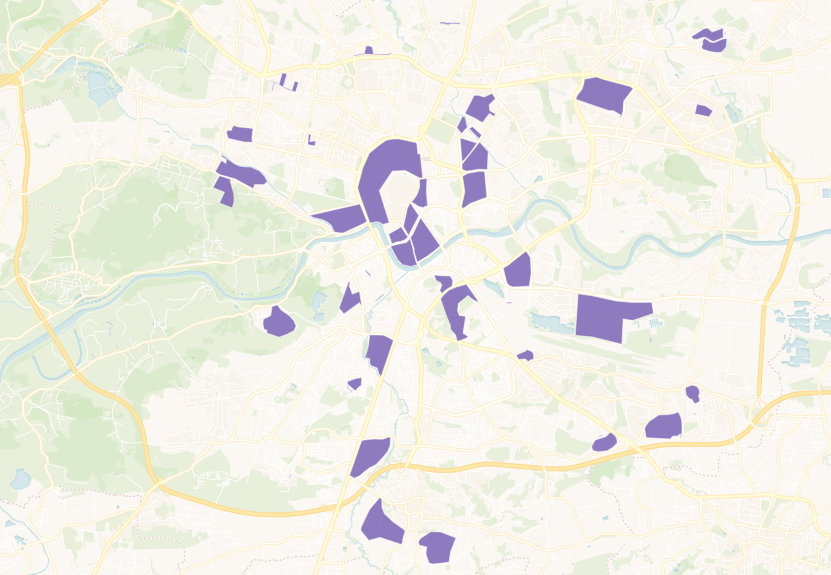
\includegraphics[width=\textwidth]{tempo30}
\caption{Strefy tzw. ulic tempo 30; źródło ZIKiT: \protect\url{https://zikit.carto.com/tables/tempo30krakow/public\#/map} (stan na dzień 6.09.2019).}
\end{figure}

Kwestia poprawnego grafu relacji to także trudny temat. Samo jego zbudowanie to jedno, wielokroć istotniejszą sprawą w kontekście nawigacji rowerowej jest waga danych ścieżek. Chodzi oczywiście o – nierzadką przecież – sytuację, gdy w dane miejsce prowadzą zarówno autonomiczne ścieżki rowerowe (rozdzielone od jezdni), te wyznaczone w torze jezdni samochodowej oraz drogi z kategorii przyjaznych rowerzyście. W jaki sposób odpowiednio dobrać wagi? Co całkowicie zrozumiałe nie mogą być one równoważne, gdyż wtedy dochodziłoby do absurdalnych sytuacji, gdy nawigacja prowadziłaby po samych drogach samochodowych tylko dlatego, że trasa po autonomicznej ścieżce rowerowa byłaby dłuższa, dajmy na to, dosłownie o parę metrów. Wagi te nie mogą być także zbyt zróżnicowane, gdyż wtedy dochodziłoby do sytuacji odwrotnych: nawigacja sugerowałaby wprawdzie trasę po samych autonomicznych ścieżkach rowerowych, ale znacznie dłuższą, niż gdyby skorzystać w paru miejscach ze „skrótu” w postaci drogi lokalnej. Stąd tak ważne jest by autorzy takiej nawigacji dobrze znali obszar ( w tym przypadku miasto Kraków), po którym ma ona prowadzić. Bez praktycznej znajomości topografii, mogłoby być ciężko wykryć pewne błędy w postaci nielogicznych tras.

\section{Istniejące rozwiązania}

Światowy rynek nawigacji rowerowych nie grzeszy obfitością, nie mówiąc już o rozwiązaniach stricte dla terenów Polski. Oczywiście funkcjonują rozwiązania gigantów jak choćby Mapy Google (zarówno wersja webowa jak i na urządzenia mobilne), czy Mapy Apple (wyłącznie na urządzenie mobilne), jednak ich główną domeną jest nawigacja przygotowana dla samochodów, odmiana dla rowerzystów, to raczej dodatek traktowany obecnie nieco po macoszemu i oparty na nie do końca sprawdzonych danych, co wyraźnie widać w ich działaniu. Dlatego też rozwiązania te wpadają w proste pułapki jak na przykład wyznaczanie trasy przez schody bądź pomijanie tzw. kontrapasów rowerowych. Nie ma się jednak temu co dziwić, jeśli weźmiemy pod uwagę ogrom obszaru jaki obejmują niniejsze projekty. Niemałym problemem w ich przypadku jest również mocne opóźnienie aktualizacji w stosunku do rzeczywistych zmian w infrastrukturze. Istnieją oczywiście również profesjonalne urządzenia nazywane „nawigacją rowerową”, jednak są to produkty dość drogie i skierowane raczej do co najmniej średnio-zaawansowanych rowerzystów, a nie do człowieka, który po prostu chce dostać się do pracy przy pomocy rowery. Inną sprawą jest, ze tego typu profesjonalne nawigacje starają się za wszelką cenę unikać zatłoczonych tras i większych miast, siłą rzeczy więc nie nadają się do nawigowania po metropoliach. \newline
Osobnym przypadkiem jest aplikacja Bike Citizens, dostępna zarówno w formie webowej jak i na urządzenia mobilne. U podstaw tego austriackiego projektu leży wyznaczanie trasy dla rowerzystów, co zresztą sugeruje już jej angielska nazwa. Co więcej, swoje działanie ogranicza jedynie do wybranych europejskich miast (obecnie jest ich około 450), co pozwala mieć nadzieję na poprawniejsze wyniki niż masowe rozwiązania. I faktycznie, choć Bike Citizens korzysta z danych OpenStreetMap, to jednak mocno je modyfikuje dzięki czemu, są całkiem obszerne i precyzyjne. Efektem tego aplikacji zdarza się wyznaczać trasy znacznie lepsze niż opisywane wyżej rozwiązania informatycznych gigantów. Niestety kluczowym jest sformułowanie „zdarza się”. Bike Citizens zbyt często popełnia błędy projektów o zbyt dużej skali, największe problemy mając z odpowiednim dopasowaniem wag, co skutkuje nadgorliwym prowadzeniem po ścieżkach rowerowych (przez co trasa potrafi być przesadnie długa). Jej dużą wadą jest też oparcie się o OpenStreetMap. Wprawdzie jej dane są zazwyczaj bardzo aktualne, a dodatkowo Bike Citizens samo je jeszcze poprawia (z różnym skutkiem z powodu – jak zostało napisane wyżej – zbyt dużej skali), to jednak fakt tworzenia ich przez zwykłych użytkowników, a nie ludzi obeznanych z tematem, ma kilka niekorzystnych następstw. Po pierwsze dane potrafią być bardzo niespójne. Istnieje także ryzyko dużych przekłamań względem rzeczywistości, czy po prostu próby nieśmiesznego żartu w postaci wprowadzenia celowo zupełnie bezsensownych danych. Wprawdzie takie odchyłki zostają szybko wyłapywane i poprawiane, jednak stwierdzenie „szybko” może oznaczać nawet parę dni, w trakcie których ktoś może się bardzo zdziwić wyznaczając trasę przy pomocy aplikacji.\newline
Istnieją jeszcze pojedyncze projekty, które starają się nawigować rowerzystów (lub choćby wyznaczać dla nich trasę) jak Mapa Polski, naviki czy Locus Mapa. Jednak wszystkie te rozwiązania są oparte na którymś z wyżej wymienionych projektów, nie dokładając wiele od siebie, a często oferując gorsze algorytmy wyszukiwania, czy mniej intuicyjny interfejs. 

\chapter{Charakterystyka środowisk}
\label{cha:charakterystyka_srodowisk}

Stworzenie autonomicznej, w pełni funkcjonalnej aplikacji wiąże się z wykorzystaniem wielu różnorodnych języków programowania, środowisk, baz danych i narzędzi. Odpowiednio szeroka wiedza na ich temat jest konieczna by móc w pełni skorzystać z ich potencjału. Inna kwestią jest umiejętne ich wybranie - tak by pasowały do potrzeb konkretnego projektu - oraz użycie, co niejako jest gwarantem ostatecznego sukcesu. Stąd też w kolejnych podrozdziałach pokrótce scharakteryzowane zostaną wszelkie udogodnienia, które zostały wykorzystane w celu implementacji nawigacji rowerowej. 

\section{Urządzenia mobilne z systemem iOS}

Od dłuższego czasu wyraźnie widać, że na rynku urządzeń mobilnych funkcjonują w zasadzie tylko dwa systemy operacyjne: Android oraz iOS. Zdecydowanie popularniejszy jest ten pierwszy, jednak i drugi ma niemałe grono oddanych użytkowników. iOS posiada jednak kilka atutów i niezaprzeczalnych zalet, które mocno odróżniają go od konkurenta. Przede wszystkim jest on w pełni zamkniętym systemem, którego twórca – amerykańska firma Apple – stworzyła bazując na własnym systemie operacyjnym Mac OS X. Ten ostatni powstał pod koniec XX wieku i napędzał komputery osobiste typu Macintosh. Oba te systemy bazują de facto na systemie Darwin, który z kolei ma Unixowy rodowód i jest oparty o jądro Mach, opracowane na amerykańskim Uniwersytecie Carnegie-Mellon. 
Sam system iOS zadebiutował wraz z premierą pierwszego iPhone'a, która odbyła się 9 stycznia 2007 roku na wystawie Macworld w San Francisco. Wówczas system ten był po prostu dostosowaną do realiów sprzętu mobilnego wersją systemu Mas OS X i nie posiadał własnej nazwy. Ta została nadana dopiero ponad rok później, w marcu 2008 roku i brzmiała iPhone OS. Po nieco ponad dwóch latach korporacja z Coupertino zdecydowała o jej skróceniu do formy iOS, która to nie zmieniła się już do czasu obecnego.
Jak wspomniano wcześniej system iOS jest systemem całkowicie zamkniętym i jedynym podmiotem, który oficjalnie mógł i może go modyfikować jest firma Apple, co z automatu powoduje, że jest ona również jedyną firmą, która może oferować sprzęt z preinstalowanym niniejszym systemem. Decyzja o wprowadzeniu takiej hermetyczności systemu miała swoje silne podwaliny w planach na firmowe portfolio produktów. Mianowicie amerykańska korporacja chciała wypuszczać na rynek pojedyncze urządzenia o konkretnej (w obrębie danej generacji) specyfikacji sprzętowej, dzięki czemu system można było bardzo mocno optymalizować. Plany zostały zrealizowane, a telefony czy też tablety z logo nadgryzionego jabłka stały się synonimem szybkości i stabilności działania, czego zdecydowanie nie można powiedzieć nawet o najdroższych urządzeniach z systemem Android.
System iOS złożony jest z 4 warstw abstrakcyjnych (logicznych): Core OS, Core Services, Media oraz Cocoa Touch. Najniższą jest Core OS, na którą składa się między innymi hybrydowe jądro Darwin, a jej rolą jest zapewnienie odpowiedniej interakcji między sprzętem a oprogramowaniem. Core Services jest zbiorem bazowych bibliotek, które zarządzają pracą wielu podstawowych funkcji,  niedostrzegalnych jednak bezpośrednio dla końcowego użytkownika, jak np. praca wątków i aplikacji, obsługa baz danych czy sieci. Za obsługę obrazu oraz dźwięku odpowiada warstwa Media, a w jej skład wchodzą między innymi biblioteki OpenGL czy Core Animation. Natomiast o poprawne działanie interfejsu użytkownika przy użyciu ekranu dotykowego dba warstwa Cocoa Touch. 

\section{Środowisko webowe}

Internet jest obecnie tak powszechnym medium, że wiele ludzi w ogóle nie wyobraża sobie bez niego codziennego funkcjonowania. Faktem jest, że jego popularyzacja ułatwiła dostęp do ogromnej bazy informacji (inną sprawą jest odpowiednie odsianie tych nieprawdziwych od prawdziwych) oraz komunikację między ludźmi. Jednak korzystacie z zasobów internetu nie byłoby możliwe – lub, co bliższe prawdzie, byłoby znacznie utrudnione – gdyby nie przeglądarki internetowe. Na rynku jest ich bardzo dużo, dostępne są na niemal każdy możliwy system operacyjny, a różnić się mogą zarówno wyglądem, funkcjonalnością, jak i silnikiem do renderowania stron. \newline
Najpopularniejszymi obecnie przeglądarkami na świecie są Google Chrome, Safari, Mozilla Firefox, UC Browser, Samsung Internet Browser, Opera, Internet Explorer oraz Edge. Zmianę ich rynkowego udziału w ostatniej dekadzie widać na obrazku Rys. 4.1.

\begin{figure}[H]
\centering
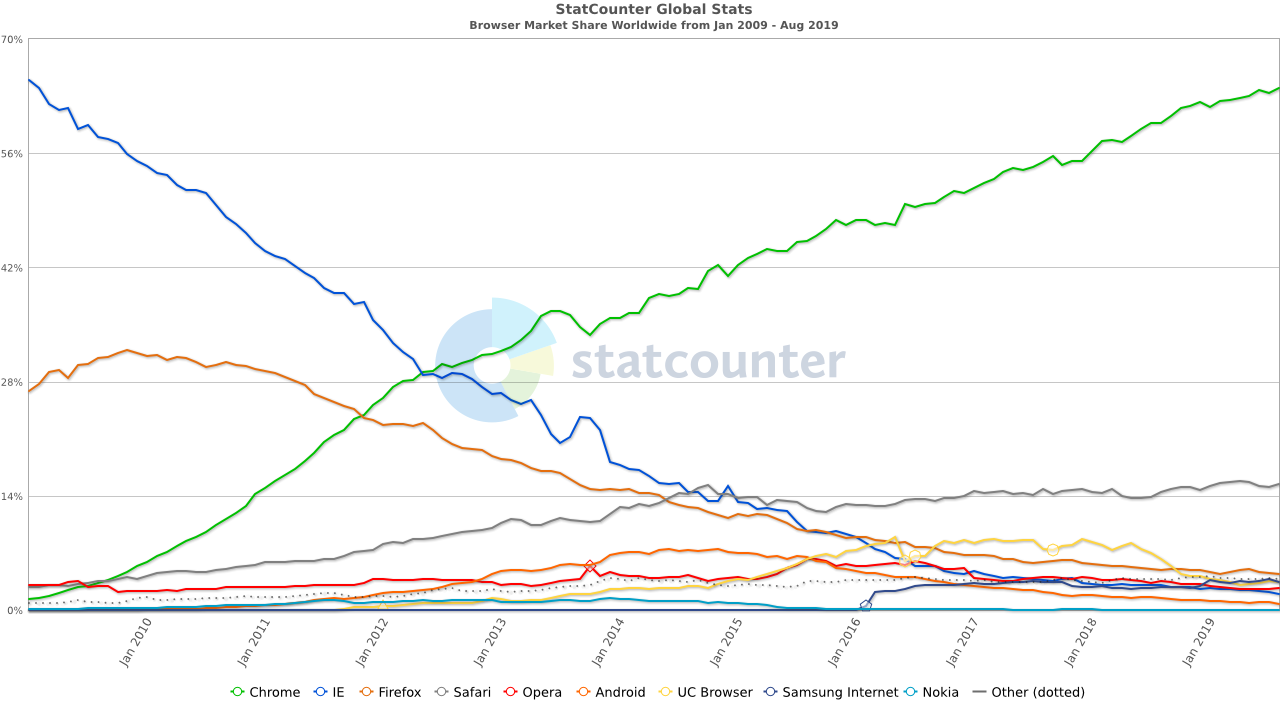
\includegraphics[width=\textwidth]{przegladarki_stats}
\caption{Statystyki użycia przeglądarek internetowych według witryny \protect\url{https://gs.statcounter.com/browser-market-share\#monthly-200901-201908} (stan na dzień 6.09.2019).}
\end{figure}

Jak widać Google Chrome mocno dominuje nad konkurencją, a pierwsze trzy przeglądarki mają w swych rękach ponad 80\% światowego rynku, dlatego też to właśnie one – jako te zdecydowanie najczęściej używane – zostaną poniżej pokrótce omówione.\newline
Google Chrome jest produktem firmy Google. Pierwsze jej wydanie miało miejsce 2 września 2008 roku i opierało się na rozwiązaniach open source po części bazując także na innych silnikach przeglądarek internetowych, między innymi na Mozilli czy WebKit'cie. Od wersji 28 wydanej w czerwcu i lipcu 2013 roku (w zależności od systemu) Chrome zaczął korzystać z własnego silnika Blink, opracowanego przez Google, a który jest forkiem komponentu WebCore silnika WebKit. Cechą charakterystyczną tej przeglądarki zawsze był minimalistyczny interfejs, a w początkach jej istnienia także rozdzielenie zakładek na osobne procesy, co wówczas było rozwiązaniem niespotykanym. Obecnie Google Chrome jest dostępny jako darmowa aplikacja na systemy Linux, Windows, macOS, Android oraz iOS.\newline
Drugą najpopularniejszą przeglądarką internetową jest produkt firmy Apple o nazwie Safari, której debiut odbył się 7 stycznia 2003 roku. Występowała ona wyłącznie na urządzeniach amerykańskiej firmy, poza okresem między rokiem 2007 a 2012, kiedy to dostępna była również wersja dla systemów Windows. Safari do renderowania stron korzysta z otwartego silnika WebKit, jednak pozostała część jej kodu (między innymi GUI) jest zamknięta, dostępna wyłącznie w formie binarnych plików wykonywalnych.\newline
Ostatnią z liczących się przeglądarek jest Mozilla Firefox autorstwa Mozilla Foundation. Jest to oprogramowanie o otwartym kodzie źródłowym wykorzystujące silnik Gecko, który również jest dziełem Mozilli. Jej pierwsze wydanie o numerze 0.1 datuje się na 23 września 2002 roku. Tym co wyróżniało Firefoxa na tle innych przeglądarek było łatwa możliwość modyfikacji, a co za tym idzie mnóstwo dostępnych dodatków, podzielonych na trzy kategorie: motywy, rozszerzenia oraz wtyczki. Program Mozilli był w zasadzie pierwszym, który udostępniał taką możliwość, czym rozpoczął modę na tego typu dodatkowe udogodnienia. Później podobne rozwiązania wprowadził między innymi Google Chrome czy Opera.

\section{Dane geoprzestrzenne}

Nie ma chyba ważniejszego aspektu w przypadku jakiejkolwiek aplikacji mającej na celu wyszukiwanie tras, niż dysponowanie odpowiednimi danymi obszaru, po którym chcemy nawigować. Oczywiście kluczowymi są dane geograficzne, ale zazwyczaj tego typu zbiory danych zawierają także wiele innych cennych informacji, stąd określa się je ogólnie jako dane geoprzestrzenne. Bazy tego typu danych są absolutnie niezbędne do stworzenia oprogramowania takiego rodzaju, jakiego podjęto się w niniejszej pracy.


\subsection{Dane urzędu miasta krakowa na temat ścieżek rowerowych (CartoDB)}

Głównym źródłem danych, którymi posiłkuje się stworzona aplikacja, są te na temat infrastruktury rowerowej miasta Krakowa autorstwa ZIKiTu. Dane te zebrane są w formie zbioru danych CartoDB. Jest on licencjonowany i dostarczany w tzw. modelu SaaS (z ang. Software as a Service) polegającym na subskrypcji centralnie hostowanej usługi. CartoDB idealnie nadaje się do przechowywania danych geoprzestrzennych, gdyż dokładnie w tym celu został zaprojektowany i stworzony. Opiera się on na relacyjnych bazach danych PsotgreSQL oraz PostGIS, która to dodaje do tej pierwszej obsługę danych geograficznych, dzięki czemu CartoDB obsługuje wiele formatów danych wejściowych. W realizacji projektu wykorzystano również język JavaScript (w części front-endowej aplikacji webowej) oraz Node.js (w bibliotekach oraz back-endowym API). Kreacja bazy danych przy pomocy CartoDB możliwa jest w sposób wizualny, to jest po prostu zaznaczając konkretne dane bezpośrednio na mapie. Jest to niewątpliwe sporą zaletą, gdyż ułatwia niedoświadczonym użytkownikom stworzenie bazy, a z drugiej strony także i wadą, gdyż powoduje takie problemy jak np. rozbieżność punktów sąsiadujących ze sobą elementów spowodowane zaznaczeniem minimalnie innych danych (rozdzielczość koordynat na mapie jest bardzo duża, więc nawet bardzo małe przesunięcie w miejscu na mapie, skutkuje innymi współrzędnymi geograficznymi).\newline
Same dane ZIKiTu obejmują swym zasięgiem jedynie gminę Kraków, lecz są całkiem obszerne i dokładne, choć rzadko aktualizowane. Poniżej można zobaczyć strukturę pojedynczego rekordy z niniejszej bazy na przykładzie Małego Rynku: \newline

\lstset{language=XML, breaklines=true}
\begin{lstlisting}
<Placemark>
<Style><LineStyle><color>ff0000ff</color></LineStyle><PolyStyle><fill>0</fill></PolyStyle></Style>
 <ExtendedData><SchemaData schemaUrl="\#infrastruktura_rowerowa_06_2018">
  <SimpleData name="cartodb_id">640</SimpleData>
  <SimpleData name="kategoria">c16t22-e</SimpleData>
  <SimpleData name="opis">Maly Rynek</SimpleData>
  <SimpleData name="dlugosc"></SimpleData>
  <SimpleData name="data"></SimpleData>
  <SimpleData name="szerokosc"></SimpleData>
  <SimpleData name="nawierzchnia">kostka brukowa</SimpleData>
  <SimpleData name="informacje_dodatkowe">kontraruch od Mikołajskiej do Siennej </SimpleData>
 </SchemaData></ExtendedData>
<MultiGeometry><LineString><coordinates>19.939853,50.060845 19.940441,50.06162 19.940424,50.061682</coordinates></LineString></MultiGeometry>
</Placemark>
\end{lstlisting}

Niestety można zauważyć pewien problem – a przynajmniej problem z punktu widzenia programisty chcącego stworzyć poprawny graf relacji opierając się na danych z niniejszej bazy – wynikający ze wspomnianego wcześniej graficznego tworzenia bazy. Otóż każda ulica czy ścieżka składa się w niej ze zbioru punktów, każdy określony współrzędnymi geograficznymi. Taki zbiór punktów nazywamy segmentem. Pierwszą niedogodnością jest fakt, że współrzędnego geograficzne punktów początkowych różnych segmentów w miejscu ich skrzyżowania delikatnie się od siebie różnią. W terenie różnice te sięgają co najwyżej kilku centymetrów, jednak od strony projektowej powodują konieczność wprowadzenia promienia wyszukiwania sąsiadujących punktów w momencie skrzyżowania się segmentów, gdyż bez tego nie dałoby się stworzyć spójnego grafu (precyzyjnie ujmując zawierałby on ledwie jeden segment – ten pierwszy, gdyż teoretycznie żaden segment nie byłby połączony z innym). Jednak powyższe zjawisko samo w sobie nie wydaje się nastręczać ogromnych problemów, zdecydowanie gorzej jest gdy dodamy do niego drugą wadę. Mianowicie punkty wchodzące w skład segmentu są definiowane tylko w przypadku, gdy segment, na który się składają, ulega zmianie kierunku w sensie geograficznym. Innymi słowy jeśli segment (czyli ulica lub ścieżka itp.) jest na jakimś swym odcinku poprowadzona idealnie na wprost, to baza zawiera jedynie punkt początkowy i końcowy takiego fragmentu. Oczywiście takie rozwiązanie jest sensowne i w normalnych przypadkach nie powoduje żadnych negatywnych konsekwencji. Jednak, jeżeli np. w połowie tego idealnie prostego fragmentu znajduje się skrzyżowanie z innym segmentem, to zbudowanie grafu relacji zaczyna być niemałym wyzwaniem. 

\subsection{Dane społeczności rowerowej (DaroPlan)}

Dane zebrane przez ZIKiT, choć dokładne i obszerne, okazały się niewystarczające by umożliwić silnikowi aplikacji znalezienie odpowiednich tras w każdym rejonie Krakowa. Dlatego też do projektu zdecydowano się dodać zbiór danych DaroPlan stworzony przez organizację pozarządową Otwarty Plan. Uzupełnia ona dane zgromadzone przez miejskich urzędników i powoduje, że na mapie Krakowa znacznie ubywa białych plam, czyli miejsc bez żadnych sugerowanych tras do przejazdu przy pomocy rowery. Zbiór ten również korzysta z CartoDB i został podobnie zdefiniowany.

\subsection{OpenStreetMap oraz Apple Maps}

OpenStreetMap jest otwartą mapą całej kuli ziemskiej tworzoną przez społeczność internetową. Jest ona całkowicie darmowa i swobodnie dostępna. Stworzył ją w 2004 roku Brytyjczyk Steve Coast, który inspirował się ogromną popularnością projektu Wikipedia. Coast pragnął by dane geograficzne również były ogólnodostępne, co w czasach sprzed powstania OpenStreetMap nie miało miejsca. Edytujący mapę muszą być zarejestrowani by móc wprowadzać zmiany, a w 2018 roku takich użytkowników było na świecie ponad 4.5 miliona. Dużym atutem mapy – poza jej darmowością i dostępnością – jest jej bardzo przyjazne API. Dzięki temu na przykład taki proces jak wyciągnięcie współrzędnych geograficznych danego adresu wiąże się z napisaniem prostego zapisania do bazy danych.\newline
Mapy Apple to usługa intenretowych map stowrzona przez Apple. Powstała ona dla systemów operacyjnych iOS, macOS i watchOS (w tej chronologii), a pierwsze wydanie miało miejsce 19 września 2012 i było wersja dla systemu iOS, zastępując funkcjonujące tam dotychczas Mapy Google. Apple Maps korzystają zarówno z danych opisanej wyżej OpenStreetMap, jak i z danych dostarczanych przez holenderską firmę TomTom. To co wyróżnia Mapy Apple na tle innych podobnych rozwiązań, to zastosowanie grafiki wektorowej do wizualizowania map. Taki sposób renderowania powoduje mniejsze zużycie danych oraz szybsze działanie mapy (a w zasadzie mniejszą zapotrzebowanie na zasoby sprzętowe).

\section{Użyte algorytmy}

Podstawowym problemem przy wszelkiego rodzaju aplikacjach wyznaczających trasy, jest problem najkrótszej ścieżki. W przypadku omawianego w niniejszej pracy zagadnienia wyszukiwania tras rowerowych, najbardziej reprezentatywnym matematycznym odzwierciedleniem danych o sieci ścieżek będzie graf, którego wierzchołki będą reprezentować skrzyżowania, a krawędzi odcinki pomiędzy nimi. Wagi tychże odcinków będą oznaczały ich długość. Z tego też powodu – rzeczywistego charakteru modelu – problem ten można zawęzić do poszukiwania najkrótszej ścieżki w grafie o wagach nieujemnych. Jest tak, ponieważ w rzeczywistości nie istnieją ścieżki, których długość wyraża się w liczbie ujemnej. W jaki sposób rozwiązać powyższy problem? Najbardziej logicznym rozwiązaniem, który pierwszy przychodzi do głowy jest zsumowanie wag wszystkich odcinków wchodzących w skład każdej możliwej tras z punktu startowego do końcowego i wybranie tej trasy, której sumaryczna waga jest najniższa. Jak łatwo się jednak domyślić, takie postępowanie jest niezwykle nieefektywne i w przypadku większej ilości odcinków oraz możliwych tras pomiędzy punktami początkowym i końcowym, zupełnie traci sens, gdyż jego złożoność obliczeniowa jest ogromna. Dlatego też istotnym jest wykorzystanie odpowiednich algorytmów działania, które pomogą w sposób efektywny (w stopniu większym lub mniejszym – w zależności od konkretnego algorytmu i problemu) rozwiązać problem znalezienia najkrótszej ścieżki w grafie o wagach nieujemnych.

\subsection{Algorytm Dijkstry}

Algorytm Dijkstry został wynaleziony w roku 1956 przez Edsgera W. Dijkstra. Jest jednym z najprostszych do implementacji sposobów wyszukiwania najkrótszych ścieżek w grafie, ale przy okazji jednym z najwolniejszych w działaniu. Umożliwia wyznaczenie ścieżek w grafie ważonym, w którym waga każdej z krawędzi jest nieujemna. Działanie algorytmu polega na przekazaniu punktu początkowego a następnie wyznaczeniu najkrótszych ścieżek do wszystkich innych wierzchołków inkrementacyjnie tworząc tablicę odkrytych ścieżek w każdym z odwiedzonych wierzchołków. W przypadku gdy nowo odkryta ścieżka nie jest jeszcze zapisana w tablicy ścieżek, zostaje do niej dodana. W przypadku gdy już tam istnieje, następuje sprawdzenie czy nowo odkryta ścieżka ma wagę mniejszą czy większą od już znalezionej. W przypadku znalezienia ścieżki o wadze mniejszej, obecnie istniejąca zostaje nią podmieniona, a algorytm kontynuuje działanie.\newline
Opisane działanie algorytmu powoduje że nie skaluje się on poprawnie w przypadku grafów o dużej ilości wierzchołków i krawędzi. Dzieje się tak ze względu na fakt że nie zawęża w żaden sposób obszaru swojego przeszukiwania. Złożoność obliczeniową grafu przedstawiono poniższym wzorem:\newline

\begin{equation}
O(|V|^2)
\end{equation}
gdzie
\begin{eqwhere}[2cm]
	\item[$V$] liczba wierzchołków w grafie 
\end{eqwhere}

Na podstawie przedstawionego wzoru możemy stwierdzić, że ilość obliczeń potrzebnych na wyznaczenie ścieżki rośnie eksponencjalnie wraz ze wzrostem ilości wierzchołków w badanym grafie.

\subsection{Algorytm A*}

Algorytm A* jest specjalną odmianą algorytmu Dijkstry, który wraz z przechodzeniem przez wierzchołki stara się optymalizować heurystykę przekazaną jako jeden z parametrów algorytmu. Przy przejściu przez każdy z wierzchołków, na podstawie informacji odnośnie poprzedniego i kolejnego przechodzonego wierzchołka, heurystyka wyznaczana jest na nowo co pozwala ominąć niektóre z nich. W przypadku gdy przekazana heurystyka jest stałą, algorytm wykazuje działanie identyczne do algorytmu Dijkstry. Z przekazanego opisu możemy odczytać że złożoność obliczeniowa algorytmu w znacznym stopniu zależy od złożoności obliczeniowej przekazanej heurystyki. Przykładowo w przypadku gdy wymaga ona iteracji po wszystkich wierzchołkach zawartych w grafie, wyznaczenie ścieżki staje się bardzo złożone. Algorytm A* jest szczególnie użyteczny w grafach posiadających swoje rzeczywiste odzwierciedlenie, jak na przykład mapę, w takim przypadku wyznaczenie heurystyki posiada liniową złożoność obliczeniową i uzyskany wynik jest bardzo dokładny.
W przeciwieństwie do algorytmu Dijkstra, algorytm A* umożliwia przeszukiwanie grafów nieskończonych, a także skaluje się dobrze dla grafów o bardzo dużej ilości wierzchołków i krawędzi. Algorytm kończy swoje działanie po odnalezieniu drogi którą uzna za optymalną, nie wymaga przeszukania reszty wierzchołków w przypadku wyspecyfikowania odpowiednio dokładnej funkcji heurystyki. Ogólną złożoność obliczeniową algorytmu A* przedstawiono poniższym wzorem:\newline

\begin{equation}
O((|V| + |E|) log |V|)
\end{equation}
gdzie
\begin{eqwhere}[2cm]
	\item[$V$] liczba wierzchołków w grafie 
	\item[$E$] liczba krawędzi w grafie 
\end{eqwhere}

W aplikacjach, w celach porównawczych, zaimplementowano jeszcze kilka innych metod wyznaczania najkrótszych ścieżek. Wszystkie jednak są pewnymi modyfikacjami algorytmu A*, a różnice zostały opisane podczas analizy.

\section{Metoda Haversine}

Metoda Haversine jest algorytmem służącym do wyznaczania odległości w linii prostej pomiędzy dwoma punktami znajdującymi się na sferze. W przypadku projektu będącego częścią tej pracy została wykorzystana do wyznaczania odległości pomiędzy punktami na mapie. Wyznaczone odległości zakładają pewną niedokładność, jako że ziemia nie jest idealną sferą. Jednak średni błąd wyznaczenia odległości przy użyciu metody Haversine jest tak mały że może zostać zignorowany przy założeniu skali długości wyznaczanych dróg mających zazwyczaj kilkaset lub więcej metrów długości.\newline
Obliczenia odległości sprowadzają się do rozwiązania równania (4.3)

\begin{equation}
d=2*r*arcsin*\sqrt{sin^2(\frac{\varphi_{2}-\varphi_{1}}{2}) + cos(\varphi)*cos(\varphi)*sin^2(\frac{\lambda_{2}-\lambda_{1}}{2})}
\end{equation}
gdzie
\begin{eqwhere}[2cm]
	\item[$d$] odległość
	\item[$r$] promień sfery
	\item[$\varphi_{1}$] szerokość geograficzna pierwszego z punktów 
	\item[$\varphi_{2}$]  szerokość geograficzna drugiego z punktów 
	\item[$\lambda_{1}$] długość geograficzna pierwszego z punktów 
	\item[$\lambda_{2}$] długość geograficzna drugiego z punktów
\end{eqwhere}

\section{Użyte języki programowania}

W celu stworzenia aplikacji serwerowej i strony www użyto szeregu bibliotek open-source. Ich zastosowanie pozwala na zdecydowaną redukcję ilości kodu potrzebnego w celu osiągnięcia oczekiwanego elementu. Każda z użytych bibliotek jest to osobna technologia, wymagająca użycia odrębnego języka programowania. W poniższych paragrafach opisano w skrócie wszystkie języki programowania oraz technologie użyte podczas pisania aplikacji będących elementem tej pracy.

\subsection{Język programowania JavaScript}

Javascript jest to skryptowy, wysoko poziomowy język programowania który jest aktualnie jednym z głównych języków programowania używanych przy pisaniu stron internetowych. Swoją popularności zyskał faktem, że aplikacje internetowe stworzone przy jego użyciu są renderowane po stronie klienta, nie serwera, co znacznie odciąża zasoby potrzebne do ich obsługi. Javascript bazuje na paradygmacie programowania funkcyjnego i imperatywnego.\newline
Od swojego powstania, w roku 1955, język bardzo ewoluował a z jego elastyczności korzysta wiele technologi często zupełnie nie związanych z tworzeniem interfejsów użytkownika w stronach internetowych. W obecnej chwili, wraz biblioteką Node.js oraz kilkoma mniej popularnymi, jest używany do pisania aplikacji serwerowych nastawionych głównie na szybkie reakcje i działanie w czasie rzeczywistym. W niedalekiej przeszłości znalazł nawet zastosowanie w pisaniu hybrydowych aplikacji mobilnych, w środowisku React Native, gdzie po napisaniu jest tłumaczony do kodu natywnego dla każdej z wybranych platform mobilnych.\newline
Jako ciekawostkę można przekazać, że język JavaScript, pomimo podobnej nazwy, nie ma nic wspólnego językiem programowania Java. Jego wypuszczenie na świat zbiegło się w czasie ze znaczną popularnością języka Java, a autorzy chcieli, nazywając go w ten sposób, sztucznie zwiększyć jego popularność.

\subsection{Język programowania Swift}

Język Swift jest funkcyjnym, statycznie typowym językiem programowania wypuszczonym przez firmę Apple w roku 2014 w celu zastąpienia przestarzałego języka Objective-C. Jest bardzo nowoczesnym językiem który od swojego początku co roku zdobywa nowe aktualizacje, często znacznie zmieniające jego działanie. Jest stworzony z myślą o pisaniu bezpiecznego kodu, który w czasie kompilacji będzie wykonywał znaczną ilość weryfikacji sprawdzających czy kod napisany przez użytkownika nie tylko będzie działał, ale także działał poprawnie. Jednym z przykładów tego zachowania są zmienne typu \textit{Optional} które przy poprawnym użyciu praktycznie uniemożliwiają odniesienie się do zmiennej która nie istnieje w pamięci i wywołania wyjątku null pointer. Język natychmiast po wprowadzeniu zgromadził wokół siebie ogromną ilość fanów, którzy zaczęli tworzyć rozszerzenia do oferowanych przez niego bibliotek oraz własne rozwiązania typu open-source.\newline
Swift został początkowo stworzony jako język do pisania aplikacji mobilnych na systemy operacyjne iOS oraz OS X dystrybuowane przez firmę Apple. Szybko jednak zdecydowano się na udostępnienie go jako open-source, oraz dodanie kompatybilności oraz kompilatora pod inne systemy bazujące na unix. Obecnie, poza tworzeniem aplikacji na urządzenia firmy Apple, Swift znalazł zastosowanie także jako biblioteka do tworzenia aplikacji internetowych korzystając przy tym z bibliotek takich jak \textit{Vapor} czy \textit{Kitura}.

\subsection{Biblioteka ReactJS}

Jedną z głównych bibliotek, używanych do tworzenia interfejsów użytkownika w aplikacjach internetowych jest biblioteka ReactJS. Jest to stosunkowo nowa technologia, wdrożona przez firmę Facebook w roku 2003. Po swojej premierze natychmiast zyskała wielu zwolenników a wiele firm zaczęło ją traktować jako główną technologię i przepisywać swoje istniejące rozwiązania. Przyczyną tego była prostota pisania kodu, stabilność i fakt zdecydowania się na obsługę jednego z najbardziej popularnych języków programowania w obecnym czasie. Biblioteka korzysta ze wszystkich standardowych funkcji języka Javascript do tworzenia logicznych części aplikacji, oraz wprowadza nowy standard deklaratywnego tworzenia interfejsów przy użyciu autorskiego rozwiązania - składni \textit{JSX}. \textit{JSX} umożliwia szybkie tworzenie widoku strony internetowej korzystając przy tym z predefiniowanych przez bibliotekę React elementów takich jak widok, tekst, tabela itp.. Stworzone aplikacje bazują na zmiennej aktualnego stanie - jest to zestaw zmiennych zdefiniowanych przez zmienną o nazwie \textit{state} w każdym z widoków. W przypadku zmiany któregokolwiek z elementów obiektu, następuje wywołanie metody render, która powoduje przeładowanie widoku. Renderowanie widoku jest możliwe dzięki React DOM. Jest to narzędzie które na podstawie przekazanego kodu JSX tworzy drzewo widoków obecnych w aktualnie wyświetlanym interfejsie, następnie przy każdej aktualizacji przelicza które z elementów powinny zostać zmienione aby poprawnie wyświetlić widok, dostosowując się do aktualnego stanu. Dzięki użyciu React DOM aplikacje stworzone przy użyciu ReactJS są bardzo wydajne.

\subsection{Biblioteka Node.js}

W celu implementacji aplikacji serwerowej użyto biblioteki Node.js, jest to stosunkowo nowa technologia, jej pierwsza wersja ujrzała światło dzienne w roku 2009. Node.js umożliwia wykonywanie kodu Javascript poza przeglądarką użytkownika, po stronie serwerowej, składa się z silnika V8 zaimplementowanego przez firmę Google oraz zestawu bibliotek dołączonych przez twórcę bilioteki w celu stworzenia wieloplatformowego środowiska do uruchamiania skryptów napisanych w kodzie Javascript. Biblioteka Node.js jest zaimplementowana w oparciu o architekturę \textit{event-driven} i asynchroniczne operacje wyjścia i wejścia, co oznacza, że biblioteka wydajnie wykorzystuje wielowątkowość i nie zostaje zablokowana wykonywaniem długich operacji przez równolegle działające procesy. Zważając na opisane wcześniej charakterystyki, oprogramowanie stworzone przy użyciu Node.js wyróżnia się dużą wydajnością oraz jest optymalnym wyborem dla aplikacji oczekujących szybkiego przetwarzania lub komunikacji w czasie rzeczywistym. Dodatkową zaletą biblioteki Node.js jest fakt, że wykorzystuje ten sam język programowania, którego używa się do programowania stron internetowych, z racji tego bariera wejścia do tworzenia pełnych systemów jest znacznie mniejsza.

\section{Użyte narzędzia}

W celu stworzenia aplikacji serwerowej oraz aplikacji mobilnej został użyty narzędzi programistycznych. Każda z użytych technologii korzysta z osobnego, często dedykowanego środowiska programistycznego, czyli aplikacji z wbudowanym edytorem tekstu przystosowanym do danego języka oraz debuggerem. Aby umożliwić sprawne tworzenie aplikacji w zespole użyto także odpowiednich aplikacji do testowania oraz systemu kontroli wersji. Wszystkie użyte przy tworzeniu oprogramowania technologie i narzędzia zostały opisane w poniższych paragrafach.

\subsection{Środowisko programistyczne Xcode}

Aplikacja na system iOS została stworzona przy użyciu środowiska programistycznego Xcode. Jest to rozbudowana aplikacja, opublikowana i rozwijana przez firmę Apple, głównie w celu tworzenia aplikacji pod systemy operacyjne iOS oraz OS X. Umożliwia jednak także kompilację języków C oraz C++ dzięki wbudowanym kompilatorom LLVM i GCC. W celu debugowania, środowisko używa debuggera LLDB, który w bardzo prosty, graficzny sposób przedstawia konsolę oraz umożliwia zatrzymanie egzekucji programu w danej linijce kodu, przechodzenie pomiędzy kolejnymi linijkami oraz cały zestaw zaawansowanych komend umożliwiających prezentację logów i egzekucję kodu implementowanego przez aplikację. Środowisko składa się z zaawansowanego edytora tekstu z wbudowaną obsługą składni języków Swift, Objective-C, C oraz C++. Poza standardową edycją podpowiadającą auto-uzupełnianie nawiasów i odpowiednie wcięcia, opisywane środowisko ma także wbudowany świetnie działający system auto-uzupełniania kodu. Jest to funkcjonalność niezmiernie przydatna jako że języki proponowane przez firmę Apple bazują na bardzo opisowej składni gdzie często jedna metoda jest długości nawet kilku linii kodu.\newline
Środowisko programistyczne Xcode ma także wbudowane system uruchomieniowy umożliwiający włączenie oprogramowania na realnym urządzeniu - komputerze lub telefonie. W przypadku braku realnego urządzenia z systemem iOS, możliwe jest także użycie symulatora dowolnego z urządzeń z dowolną wersją systemu operacyjnego. W celu instalacji aplikacji w systemie iOS na rzeczywistym urządzeniu jest jednak wymagane posiadanie opłacanego konta \textit{Apple Developer} oraz stworzenie w portalu odpowiednich certyfikatów.

\subsection{Narzędzie do testowania API Postman}

Aplikacja serwerowa udostępnia interfejs programistyczny umożliwiający dostęp do zasobów z zewnętrznych źródeł. Został stworzony w celu integracji aplikacji mobilnej. Aby umożliwić odpowiednie testowanie oraz wymianę danych testowych pomiędzy programistami pracującymi nad projektem użyto aplikacji Postman. Jest to prosta w użyciu aplikacja stworzona przez firmę Google w środowisku Electron. Umożliwia wykonywanie zapytań pod podany adres URL oraz daje interfejs graficzny do dodawania parametrów zapytania takich jak dane przesłane w zapytaniu lub nagłówki HTTP. \newline
W celu wymiany danych testowych pomiędzy osobami pracującymi nad projektem, występuje także możliwość eksportowania zestawu zdefiniowanych zapytań a następnie importowaniu ich w aplikacji u drugiej z osób.

\subsection{System kontroli wersji Git}

System git jest to rozproszony system kontroli wersji umożliwiający programistom jednoczesne tworzenie oprogramowania. Jest ono przetrzymywane w repozytorium, a dzięki mechanizmom rozgałęziania oraz ponownego scalania kodu umożliwia nawet jednoczesną edycję tych samych fragmentów kodu przez wiele osób. Poza systemem git istnieje na rynku kilka pokrewnych rozwiązań, jak na przykład system SVN, jednak w obecnej chwili git jest wiodącym oprogramowaniem z którego korzysta znaczna większość programistów i firm.\newline
Wszystkie części stworzonego systemu są przetrzymywane oraz synchronizowane przy użyciu systemu kontroli wersji git w witrynie \url{https://github.com}. Jest to jeden z najczęściej używanych hostingów do dystrybuowania aplikacji typu open-source. Dzieje się tak dzięki temu że konta nie posiadające prywatnych repozytoriów są całkowicie darmowe, niezależnie od ilości ludzi pracujących nad nimi.


\chapter{Tworzenie oprogramowania}
\label{cha:tworzenie_oprogramowania}

\section{Opis użytej technologii i bibliotek}

W celu implementacji aplikacji serwerowej użyto biblioteki Node.js, jest to stosunkowo nowa technologia, jej pierwsza wersja ujrzała światło dzienne w roku 2009. Node.js umożliwia wykonywanie kodu Javascript poza przeglądarką użytkownika, po stronie serwerowej, składa się z silnika V8 zaimplementowanego przez firmę Google oraz zestawu bibliotek dołączonych przez twórcę języka w celu stworzenia wieloplatformowego środowiska do uruchamiania skryptów napisanych w kodzie Javascript. Biblioteka Node.js jest zaimplementowana w oparciu o architekturę \textit{event-driven} i asynchroniczne operacje wyjścia i wejścia, co oznacza, że biblioteka wydajnie wykorzystuje wielowątkowość i nie zostaje zablokowana wykonywaniem długich operacji przez równolegle działające procesy. Zważając na opisane wcześniej charakterystyki, oprogramowanie stworzone przy użyciu Node.js wyróżnia się dużą wydajnością oraz optymalnym wyborem dla aplikacji oczekujących szybkiego przetwarzania lub komunikacji w czasie rzeczywistym. Dodatkową zaletą biblioteki Node.js jest fakt, że wykorzystuje ten sam język programowania, którego używa się do programowania stron internetowych, z racji tego bariera wejścia do tworzenia pełnych systemów jest znacznie mniejsza.
Aplikacja serwerowa korzysta z wielu pomocniczych bibliotek, które umożliwiają szybsze tworzenie kodu. Standardowym oprogramowaniem służącym do zarządzania zewnętrznymi bibliotekami jest aplikacja \textit{npm}, jednak podczas tworzenia tego projektu użyto aplikacji \textit{yarn}, która działa w bardzo przybliżony sposób, zabezpiecza jednak przed usunięciem przez twórcę oprogramowania kodu źródłowego każdej z bibliotek. W poniższych punktach opisano kilka wybranych bibliotek użytych do stworzenia aplikacji wraz z krótkim opisem i przykładem użycia:\newline

\textbf{Express} - biblioteka służąca do pisania aplikacji serwerowych przy użyciu biblioteki Node.js. Udostępnia prosty interfejs do tworzenia punktów końcowych i jest określana jako jeden ze standardów podczas tworzenia aplikacji serwerowych przy użyciu Node.\newline

\textbf{Eslint} - biblioteka służąca jako tzw. \textit{linter} , czyli proces na bieżąco sprawdzający jakość kodu pisanego przez użytkownika. Dzięki użyciu eslint programista nie musi martwić się o niejednorodność we wcięciach, nieużywane zmienne czy niepoprawne ilości znaków białych, jest to sprawdzane przez program. Eslint korzysta z pliku .eslintrc który definiuje wszystkie zasady które mają być spełnione w projekcie, aby kod został uznany za bezbłędny.\newline

\textbf{Axios} - biblioteka umożliwiająca proste interakcje z interfejsami serwerowymi innych serwisów. Dzięki stworzeniu globalnego klienta axios zawierającego podstawową konfigurację nie ma potrzeby powielać tych samych konfiguracji w wielu zapytaniach, wystarczy jedynie zdefiniować rzeczy, które się różnią, jak na przykład URL czy metoda HTTP.\newline

\textbf{Cors} - w celu komunikacji aplikacji serwerowej i strony internetowej znajdujących się pod jednym adresem IP należy skonfigurować \textit{„Cross Origin Resource Sharing”}. Ma to zapobiec możliwości przesyłania złośliwych skryptów w formularzach, które zostaną wykonane przez aplikację. Do umożliwienia Cross Origin Resource Sharing użyto biblioteki cors, która po inicjalizacji automatycznie dodaje nagłówek HTTP Access-Control-Allow-Origin z odpowiednią domeną, dla której tego typu zapytania mają być możliwe.\newline

Aplikacja w celu wyznaczania tras korzysta z dwóch zewnętrznych serwisów - ZiKIT Carto oraz openstreetmap. Carto jest to platforma do zarządzania danymi geoprzestrzennymi, która umożliwia pobranie, wizualizację oraz przeszukiwanie dróg przy użyciu odpowiednich komend SQL. Kod carto jest otwarty i każdy może uruchomić go w swojej stronie internetowej w celu uproszczonej wizualizacji tras na mapie. Krakowski ZiKIT korzysta z własnej instancji carto w celu wizualizacji i przetrzymywania wszelkiego rodzaju danych, takich jak zbiory różnych typów dróg oraz wydarzenia (np. wypadki samochodowe) na mapach. Openstreetmap jest to darmowy portal udostępniający usługę map oraz oferujący szeroki zakres innych danych geoprzestrzennych. Openstreetmap jest projektem otwartym, portal jest utrzymywany przez fundację o tej samej nazwie, a swoje dane zawdzięcza użytkownikom, którzy wprowadzają je w celu ich późniejszego wykorzystania lub jako wolontariusze.

\subsection{Opis udostępnionych endpointów}

W celu umożliwienia komunikacji aplikacji mobilnej oraz strony internetowej, przygotowana aplikacja serwerowa udostępnia pod zdefiniowanymi adresami URL end-point’y, które po przekazaniu odpowiednich parametrów w kwerendzie, umożliwiają pobranie danych. Zaimplementowano je przy pomocy obiektu \textit{router}, będącego częścią opisanej wcześniej biblioteki express.
Poniżej przedstawiono dwa end-point’y udostępnione przez aplikację razem z dokumentacją oraz przykładową, skróconą, odpowiedzią w formacie JSON:
\begin{enumerate}
\item Endpoint findOptimized

Używany przez aplikację mobilną w celu pobrania optymalnej trasy pomiędzy dwoma punktami przekazanymi w formie kwerendy. Wykorzystuje metodę HTTP GET. Możliwe parametry do przekazania w kwerendzie URL:

\begin{itemize}
\item startLocation - parametr określający punkt początkowy wyznaczonej trasy w przypadku, gdy jest on przekazany jako adres.
\item startLocationLatitude oraz startLocationLongitude - przez te parametry zostaje przekazana pozycja użytkownika w przypadku, gdy zostaje ona zdefiniowana przez współrzędne geograficzne punktu początkowego. Jeśli lokalizacja punktu początkowego zostaje przekazana w tej postaci, parametr startLocation zostaje zignorowany, niezależnie od tego czy został zdefiniowany w kwerendzie.
\item endLocation - parametr określający punkt końcowy trasy w postaci adresu. Aplikacja nie daje możliwości przekazania punktu końcowego trasy w postaci współrzędnych geograficznych, dlatego też w przypadku punktu końcowego trasy przekazanie lokalizacji w tej postaci nie zostało zaimplementowane.
\item routeType - określenie czy wyznaczona trasa ma być najkrótsza, czy optymalna z wagowego punktu widzenia. Przyjmuje parametr typu String o wartość BEST lub SHORTEST.
\end{itemize}

Przykładowe zapytanie HTTP GET w celu uzyskania odpowiedzi zawierającej optymalną trasę przejazdu można uzyskać pod adresem URL:

\url{bazowy_adres_url/api/routes/findOptimized?startLocation=romera&endLocation=karmelicka&routeType=BEST}

Przykładową odpowiedź, skróconą do postaci przedstawiającej jej formę przedstawiono poniżej.

\begin{center}
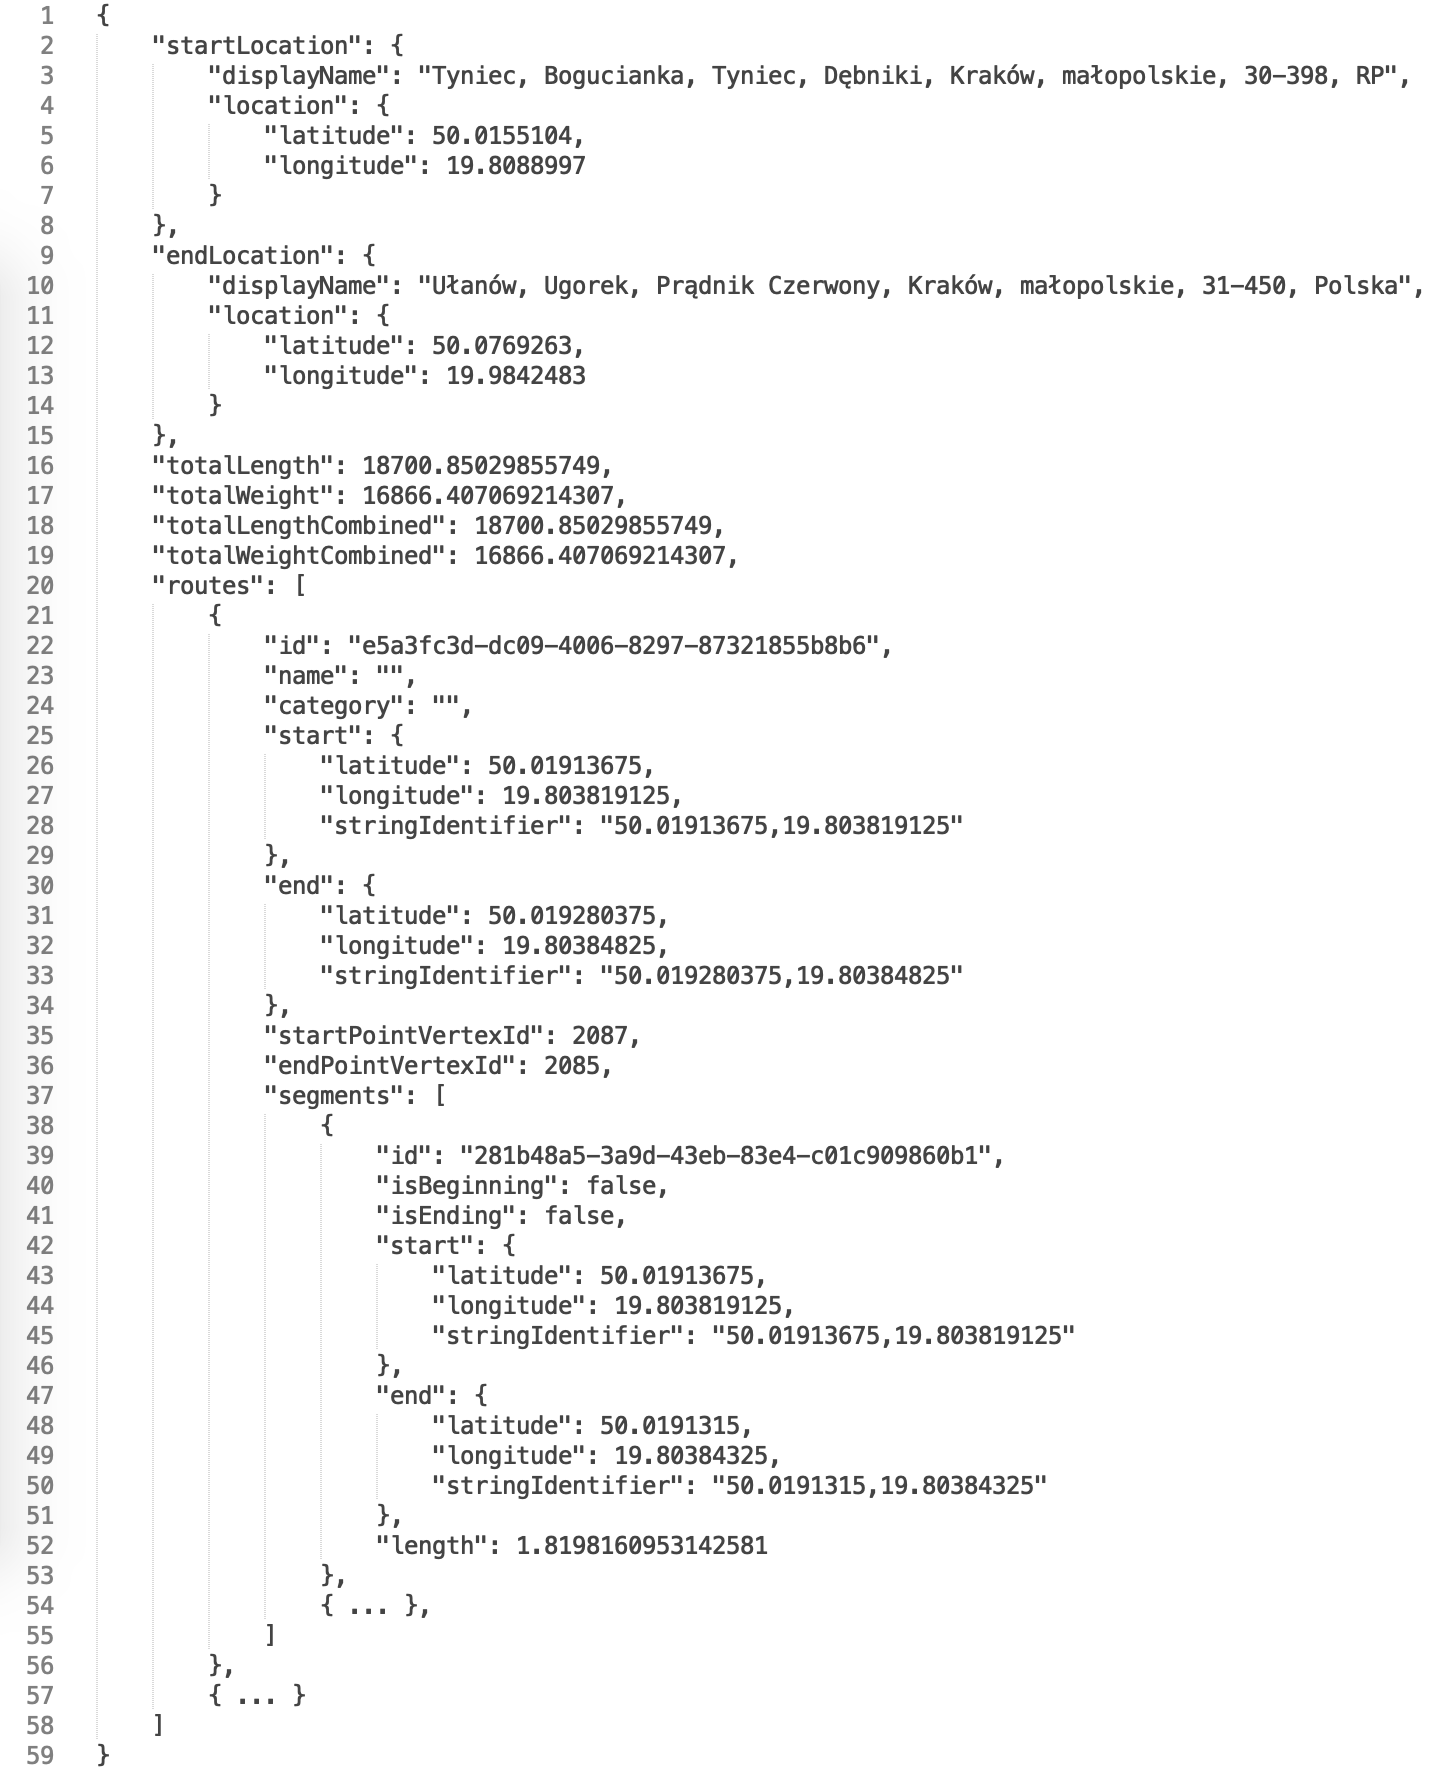
\includegraphics[height=12cm]{api_response_json}
\end{center}

\item Endpoint visualizationPoints:

Używany przez stronę internetową, będącą częścią przygotowanego systemu, w celu wizualizacji trasy na mapach openstreetmap. Wykorzystuje metodę HTTP GET. Możliwe parametry do przekazania w kwerendzie URL:

\begin{itemize}
\item startLocation - parametr określający początkową lokalizację użytkownika w postaci adresu.
\item endLocation - parametr określający końcową lokalizację użytkownika w postaci adresu.
\item routeType - określenie czy wyznaczona trasa ma być najkrótsza, czy optymalna z wagowego punktu widzenia. Przyjmuje parametr typu String o wartości BEST lub SHORTEST.
\item algorithm - parametr określający jaki algorytm ma zostać użyty do wyszukania trasy. Przyjmuje parametr typu String o wartości ASTAR, AGREEDY lub NBA.
\end{itemize}

Przykładowe zapytanie HTTP GET w celu uzyskania odpowiedzi zawierającej optymalną trasę przejazdu można uzyskać pod adresem URL:

\url{bazowy_adres_url/api/routes/visualizationPoints?startLocation=romera&endLocation=karmelicka&routeType=BEST&algorithm=ASTAR}

Przykładową odpowiedź, skróconą do postaci przedstawiającej jej formę przedstawiono poniżej:

\begin{center}
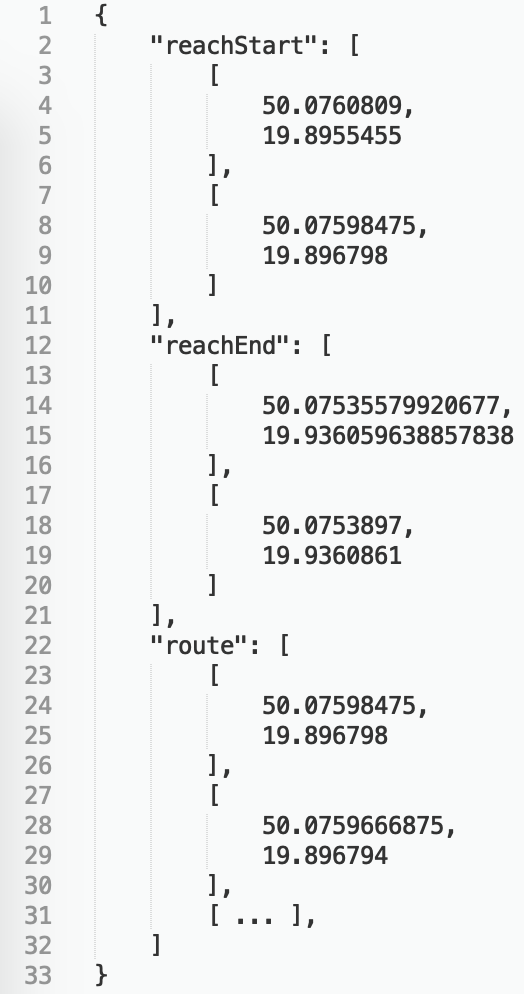
\includegraphics[height=12cm]{api_response_viz_json}
\end{center}

\end{enumerate}

\subsection{Proces wyznaczania grafu na podstawie pobranych danych}

W celu dodatkowej wizualizacji na poniższym schemacie blokowym przedstawiono proces wyznaczania grafu na podstawie pobranych danych geoprzestrzennych:

\begin{center}
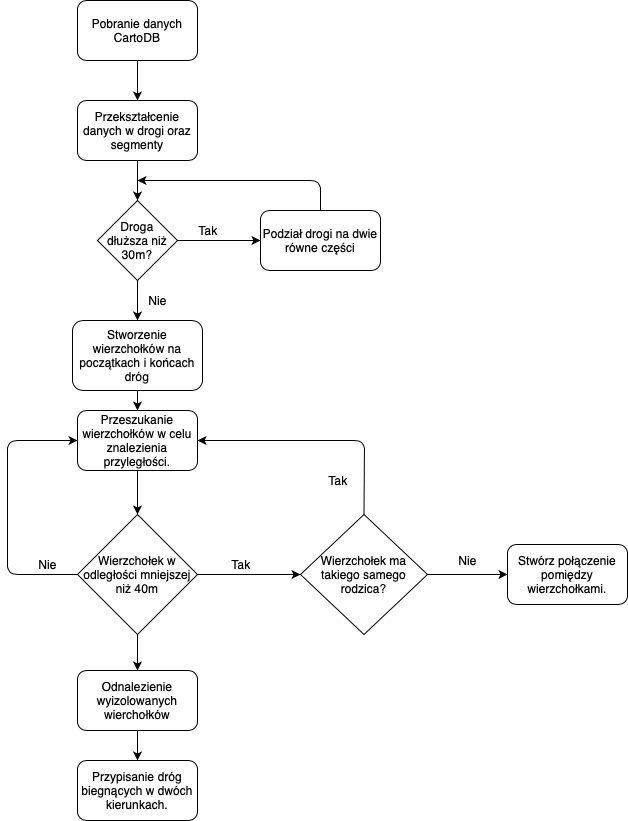
\includegraphics[width=\textwidth]{algorytm_schemat_blokowy}
\end{center}

W celu optymalizacji czasu działania systemu, dane geoprzestrzenne są pobierane oraz przetwarzane przez aplikację tylko jeden raz, zaraz po włączeniu. Jest to czasochłonny proces, wymagający wielu iteracji po rozległym zbiorze danych. Jego rezultatem jest stworzenie grafu, który może być w kolejnych etapach wykorzystywany jako gotowa dana wejściowa. Tworzenie grafu zostaje rozpoczęte przez pobranie zestawu danych geoprzestrzennych dla miasta Kraków z portalu \textit{https://zikit.carto.com}. Pobrana baza danych zawiera zarówno trasy rowerowe, jak i drogi z ograniczeniem prędkości poniżej 50 kilometrów na godzinę, obydwie bazy są następnie scalane i przekształcane w zbiór odpowiednich dróg i segmentów. Droga jest logiczną reprezentacją krzywej poprowadzonej na mapie pomiędzy dwoma punktami, składa się z segmentów, które zawierają jedynie punkt początkowy oraz końcowy i definiują zestaw linii prostych, które mogą zostać użyte, aby narysować linię drogi na mapie. Wykorzystując metodę Haversine, zostają wyznaczone długości każdej drogi przez zsumowanie długości wszystkich segmentów, które się na nią składają. \newline
Kolejnym etapem jest proces przygotowywania dróg do procesu tworzenia grafu. Aby mieć pewność, że wszystkie przyległości zostaną poprawnie odnalezione, w pierwszym kroku należy odpowiednio podzielić wszystkie pobrane drogi na takie o mniejszej długości. Trasy pobrane z serwisu Carto mają bardzo losowe długości oraz są zaznaczone w taki sposób, że nie występuje segmentacja w okolicach końców innych tras oraz przy przecięciach z nimi. Z tego powodu wyznaczenie poprawnego grafu z uzyskanych danych wymaga wcześniejszego przetworzenia. Pierwszym krokiem przetwarzania danych jest podzielenie segmentów uzyskanych z przeanalizowanych, pobranych danych na takie, które mają maksymalnie trzy metry długości. Dzieje się to przez podział każdego segmentu na pół do momentu aż osiągną one pożądaną długość. W następnej kolejności, gdy posiadamy już podzielone segmenty, następuje podzielenie tras. Dzieje się to na zasadzie podzielenia tablicy segmentów na części o określonej długości a następnie utworzenia zestawu nowych dróg z uzyskanych części. Każda droga, stworzona przez podzielenie innej drogi na mniejsze części, posiada także przypisanie swojego "rodzica", czyli pierwotnej drogi z której nastąpił podział. Droga, będąca "rodzicem", posiada za to tablicę zawierająca wszystkie drogi będące jej "dziećmi". Na tym etapie następuje także przypisanie drodze odpowiedniej wagi oraz stwierdzenie czy droga przebiega po moście - jest to stwierdzane na podstawie wykrycia słów kluczowych „most” lub „kladka” w nazwie trasy. Niestety baza danych carto ZiKiT nie oferuje w swoich danych takich informacji, dlatego też występuje potrzeba przewidzenia tej danej w inny sposób. \newline
Proces tworzenia grafu rozpoczyna się od stworzenia wierzchołka w każdym miejscu będącym zakończeniem lub rozpoczęciem drogi. W tym celu następuje iteracja po wszystkich drogach będących "rodzicami", dla każdej z nich następuje iteracja po wszystkich jej "dzieciach" i tworzone są wierzchołki na początku pierwszej drogi oraz na zakończeniu każdej następnej. Każdy z utworzonych w tym procesie wierzchołków ma także przypisywaną trasę "rodzica", który jest "rodzicem" drogi, dla której wierzchołek został stworzony. Kolejnym etapem jest wyszukanie przyległości dla każdego z wierzchołków. W tym celu następuje zagnieżdżona iteracja po wszystkich stworzonych wierzchołkach i porównywana jest odległość pomiędzy nimi. W przypadku, gdy odległość ta jest mniejsza niż 40 metrów, następuje połączenie wierzchołków drogą o typie \textit{standard link}. W tym procesie ignorowane są wierzchołki posiadające takiego samego "rodzica", w celu uniknięcia łączenia wierzchołków już ze sobą połączonych w obrębie jednej drogi. Ignorowane są także wierzchołki których trasa-rodzic znajduje się na moście, wyodrębniając z tego wyjątek, gdy aktualnie rozpatrywany wierzchołek jest początkiem lub końcem trasy, do której przynależy. Zabieg ten ma na celu uniknięcie łączenia za sobą dróg znajdujących się na różnej wysokości.
W kolejnym kroku działania algorytmu, obsługiwane są drogi dwukierunkowe, są to takie które w polu kategoria zawierają jeden z poniższych skrótów:

\begin{itemize}
\item dwr - droga rowerowa.
\item cpr - ciąg pieszo-rowerowy.
\item c16t22 - chodnik z dopuszczonym ruchem rowerowym (skrót pochodzi od identyfikatora znaku drogowego).
\item kontrapas i kontraruch - zakładamy, że w tym przypadku użytkownik może poruszać się w przeciwną stronę po ulicy, na której znajduje się dana ścieżka.
\item skróty pokrewne zawierające kombinację powyższych lub dopisek w postaci cyfry.
\end{itemize}

Każda z dróg przypisanych do każdego z wierzchołków, w przypadku gdy jest oznaczona jako dwukierunkowa, musi zostać odpowiednio przetworzona, aby algorytm wyszukiwania mógł przez nią prowadzić. W tym celu wszystkie takie drogi wychodzące z wierzchołka zostają dodane do dróg wchodzących do wierzchołka, a następnie zostają odwrócone, czyli podmieniany jest identyfikator wierzchołka początkowego oraz końcowego, współrzędne końca i początku, a także w analogiczny sposób zostaje odwrócony każdy segment przynależący do danej drogi. Ta sama procedura zostaje powtórzona w celu transformacji także dróg wchodzących do wierzchołka.
Ostatnim z kroków przygotowywania grafu jest wyodrębnienie samotnych wierzchołków. Są to wierzchołki, które znajdują się w mało zagęszczonym drogami obszarze i znajdują się zbyt daleko, aby znaleźć dla nich przyległości, pomimo że powinny one zostać znalezione. Przykładem dla tego przypadku może być droga rowerowa na mało uczęszczanej ulicy, która w pewnym momencie z braku możliwości poprowadzenia zostaje przerwana na odcinku długości 100-150m, po czym następuje jej kontynuacja w obrębie tej samej ulicy. W tym celu dla każdego z wierzchołków, który posiada tylko jedną drogę przychodzącą, zostaje przeszukana okolica najbliższych 150 metrów. W przypadku znalezienia zbyt dużej ilości przyległości, proces jest ignorowany. W przeciwnym wypadku wierzchołek zostaje z nimi połączony drogą typu \textit{isolation link}. \newline

Po przeprowadzaniu całego powyższego procesu zostaje wygenerowany graf składający się z wierzchołków, w którym drogi pełnią rolę krawędzi. Ostatnim krokiem, przeprowadzanym podczas tworzenia docelowego grafu, jest przypisanie wagi każdej z dróg. Zważając na fakt, że baza danych carto zawiera informacje odnośnie typów większości tras, aplikacja stara się przewidzieć zysk użytkownika z przebycia dłuższego dystansu znacznie bardziej komfortowymi drogami. W tym celu przypisywane są w zależności od kategorii wagi:

\begin{itemize}
\item Ddr - waga 0.7
\item Cpr - waga 0.8
\item Kontrapas, kontraruch - waga 0.8
\item C16t22 - waga 0.9
\item Standard link - w przypadku, gdy krótszy niż 10 metrów, posiada wagę 1.5. W przeciwnym wypadku waga jest równa 2.
\item Isolatation link - waga 4
\item Droga rowerowa bez kategorii - waga 1
\item Droga z bazy sugerowanych tras - waga 1.2
\end{itemize}

\subsection{Opis procesu wyznaczania trasy dla użytkownika}

Kolejnym etapem działania algorytmu jest wyszukiwanie tras na podstawie danych wejściowych przekazanych przez użytkownika. Gdy zostanie zarejestrowane zapytanie pod endpoint „findOptimized”, aplikacja odpowiednio przetwarza dane w celu uzyskania współrzędnych geograficznych punktu początkowego oraz końcowego trasy. Wykorzystywany jest do tego serwis openstreetmap, odpowiednio skonfigurowany w celu dekodowania lokalizacji znajdujących się w Krakowie. W zależności od wybranej metody przeszukiwania brany jest także pod uwagę przekazany przez użytkownika parametr routeType. W przypadku przekazania drogi typu „BEST” przy tworzeniu odpowiedniego typu obiektu „graph”, używanego później do przeszukiwania, do połączenia każdego z wierzchołków używana jest rzeczywista waga drogi, za to w przypadku przekazania drogi typu „SHORTEST” ignorowane są wagi dróg i brana pod uwagę jest tylko ich całkowita długość.\newline
W następnym etapie graf zostaje przeszukany w celu znalezienia wierzchołków znajdujących się najbliżej pozycji wybranych przez użytkownika. W celu zminimalizowania prawdopodobieństwa sytuacji w której znalezione wierzchołki znajdują się w dwóch grafach które są wobec siebie rozbieżne, są także wyszukiwane wszystkie wierzchołki znajdujące się w otoczeniu 300 metrów od wyznaczonego najbliższego. Metoda ma na celu w głównej mierze wykluczenie wierzchołków przynależących do odosobnionych dróg rowerowych, które ze względu na zbyt dużą odległość nie zostały włączone do żadnego większego grafu i są reprezentowane przez odrębny graf składający się jedynie z jednej krawędzie i dwóch wierzchołków, wyznaczających początek i koniec drogi.
Kolejnym krokiem działania algorytmu jest wyznaczenie wszystkich możliwych ścieżek pomiędzy wszystkimi odnalezionymi punktami początkowymi i końcowymi. Wykorzystywany jest do tego algorytm A*. Każda z odnalezionych ścieżek ma przypisywaną zsumowaną wagę wszystkich dróg które do niej przynależą z wagą 1 oraz sumę odległości początku i końca ścieżki w stosunku do punktów początkowego i końcowego przekazanych przez użytkownika z wagą 20. Krok ten ma na calu eliminację dróg które są najkrótsze, ale są podzbiorem innej dłuższej drogi która prowadzi użytkownika tą samą trasą. Ze wszystkich wyznaczonych dróg zostaje wybrana ta która ma najmniejszą wagę.
Następnie wyznaczona ścieżka musi zostać odpowiednio przekształcona aby zawierała jak najkrótsze połączenia pomiędzy drogami które do niej przynależą. W tym celu zostają z niej wyeliminowane segmenty początkowe i końcowe każdej z dróg w przypadku gdy wykryto że prowadzą użytkownika okrężną drogą. Ostatnim etapem jest połączenie każdego punktu końcowego każdej drogi przynależącej do danej ścieżki z punktem początkowym kolejnej prostą drogą łącząca. \newline
Wyznaczona oraz przekształcona ścieżka zostaje zwrócona użytkownikowi w formie odpowiedzi w formacie JSON zawierającej współrzędne punktów początkowego i końcowego oraz zbioru dróg podzielonych na segmenty które pomiędzy nimi prowadzą.

\section{Opis stworzonej aplikacji mobilnej}

\subsection{Opis technologii}

Aplikacja mobilna została zaimplementowana pod system iOS przy użyciu SDK dostarczonego przez firmę Apple umożliwiającego implementację aplikacji. Implementację interfejsu użytkownika umożliwia biblioteka CocoaTouch będąca jego częścią. Z racji faktu że aplikacja wykorzystuje moduł GPS w celu wyznaczania aktualnego położenia użytkownika oraz bibliotekę MapKit wchodzącą w część biblioteki CocoaTouch, w poniższych akapitach opisano działanie obydwu bibliotek wraz z przykładami użycia wewnątrz zaimplementowanej aplikacji. \newline
CoreLocation jest biblioteką wchodzącą w skład iOS SDK. Oferuje interfejs do wyznaczania lokalizacji użytkownika ale odpowiada także za obsługę wielu innych sensorów obsługiwanych przez telefon jak na przykład magnetometru, barometru, a nawet Bluetooth - do wyznaczania położenia w stosunku do urządzeń w standardzie iBeacon. Przed uzyskaniem lokalizacji użytkownika, w celu ochrony prywatności, musi zostać wyświetlony odpowiedni komunikat, w którym użytkownik wyraża zgodę na udostępnienie swojej lokalizacji dla aplikacji. W następnej kolejności, przy użyciu delegacji klasy CLLocationManager aplikacja uzyskuje co sekundę odpowiedź zwrotną zawierająca aktualną lokalizację użytkownika a także jej dokładność w metrach. Biblioteka CoreLocation jest także używana do wyznaczania kierunku w którym użytkowni skierował swój telefon. Umożliwia to płynną animację ikony roweru podczas prowadzenia użytkownika po trasie, w interfejsie użytkownika jest on skierowany w tę samą stronę na mapie, co telefon w rzeczywistości. Dodatkową funkcją biblioteki wykorzystywaną w aplikacji jest geocoding, czyli wyznaczanie współrzędnych geograficznych na podstawie wpisanego tekstu adresu lub działanie do tego odwrotne. Użyta została do tego klasa CLGeocoder będąca częścią CoreLocation. \newline
Drugą biblioteką zapewniającą działanie aplikacji iOS jest MapKit - biblioteka umożliwiająca wyświetlanie map na ekranie telefonu. Została wybrana w stosunku do map Google z racji na prostszą implementację w aplikacjach pisanych na system iOS a także fakt że jest rozwiązaniem natywnym, zaimplementowanym przez firmę Apple, nie zewnętrzną biblioteką.

\subsection{Schemat klas aplikacji mobilnej}

Za zarządzanie danymi oraz stanem aplikacji odpowiada klasa NavigationManager, jest to swojego rodzaju łącznik pomiędzy widokiem głównym a wszelkimi serwisami takimi jak klient nawigacji lub serwis zapewniający lokalizację użytkownika lub klasa odpowiedzialna za wykonywanie zapytań HTTP. Zarządza w odpowiedni sposób danymi wejściowymi oraz interakcjami użytkownika przekazanymi z ekranu głównego aby zareagować odpowiednimi akcjami i zmianą stanu który następnie przekazany do warstwy widoku przez delegację odpowiada za wyświetlenie odpowiednich danych dla użytkownika. Do odpowiedzialności klasy NavigationManager należą:

\begin{enumerate}
\item Obserwacja danych wpisywanych przez użytkownika do pól punktu startowego oraz końcowego.
\item Obsługa przycisku wyznaczenia aktualnego adresu użytkownika. Po jego wciśnięciu do klasy zostaje przekazane odpowiednie zdarzenie na które reaguje dekodowaniem aktualnej lokalizacji użytkownika na adres na mapie.
\item Pobranie trasy przy użyciu endpointu „findOptimized” po akcji użytkownika w postaci przyciśnięcia przycisku „Navigate” oraz zmianę stanu aplikacji na zaznaczenie trasy gdy zapytanie się powiedzie.
\item Włączenie oraz wyłączenie procesu nawigowania użytkownika w przypadku gdy została zatrzymana przez użytkownika lub znalazł się on w punkcie końcowym.
\item Na poniższej ilustracji przedstawiono schemat działania aplikacji razem z interakcjami pomiędzy jej komponentami:
\end{enumerate}

// tutaj idzie schemat aplikacji.

\subsection{Spis ekranów i stanów aplikacji}

Zaimplementowana aplikacja mobilna składa się z zestawu ekranów które umożliwiają użytkownikowi intuicyjne wprowadzenie parametrów trasy oraz przejście przez każdy stan nawigacji aż do doprowadzenia do końca trasy. W poniższych akapitach zestawiono przykładowe ekrany aplikacji wraz z opisem ich celu i możliwych interakcji ze strony użytkownika.
Bezpośrednio po wejściu do aplikacji, użytkownikowi zostaje przedstawiony ekran z mapą oraz dwoma polami tekstowymi, każde z nich posiada placeholder w celu zasugerowania którą z wartości należy wpisać. Po prawej stronie pola tekstowego służącego do pisania adresu początkowego znajduje się przycisk lokalizowania użytkownika. Po kliknięciu aplikacja pobiera z modułu GPS aktualną pozycję użytkownika, a następnie używając wbudowanej w iOS SDK klasy CLGeocoder wykonuje translację współrzędnych geograficznych na tekstową reprezentację adresu. Wyznaczony adres zostaje wpisany w pole tekstowe. Na poniższej ilustracji przedstawiono ekran początkowy w stanie gdy nie ma wprowadzonych danych.

\begin{center}
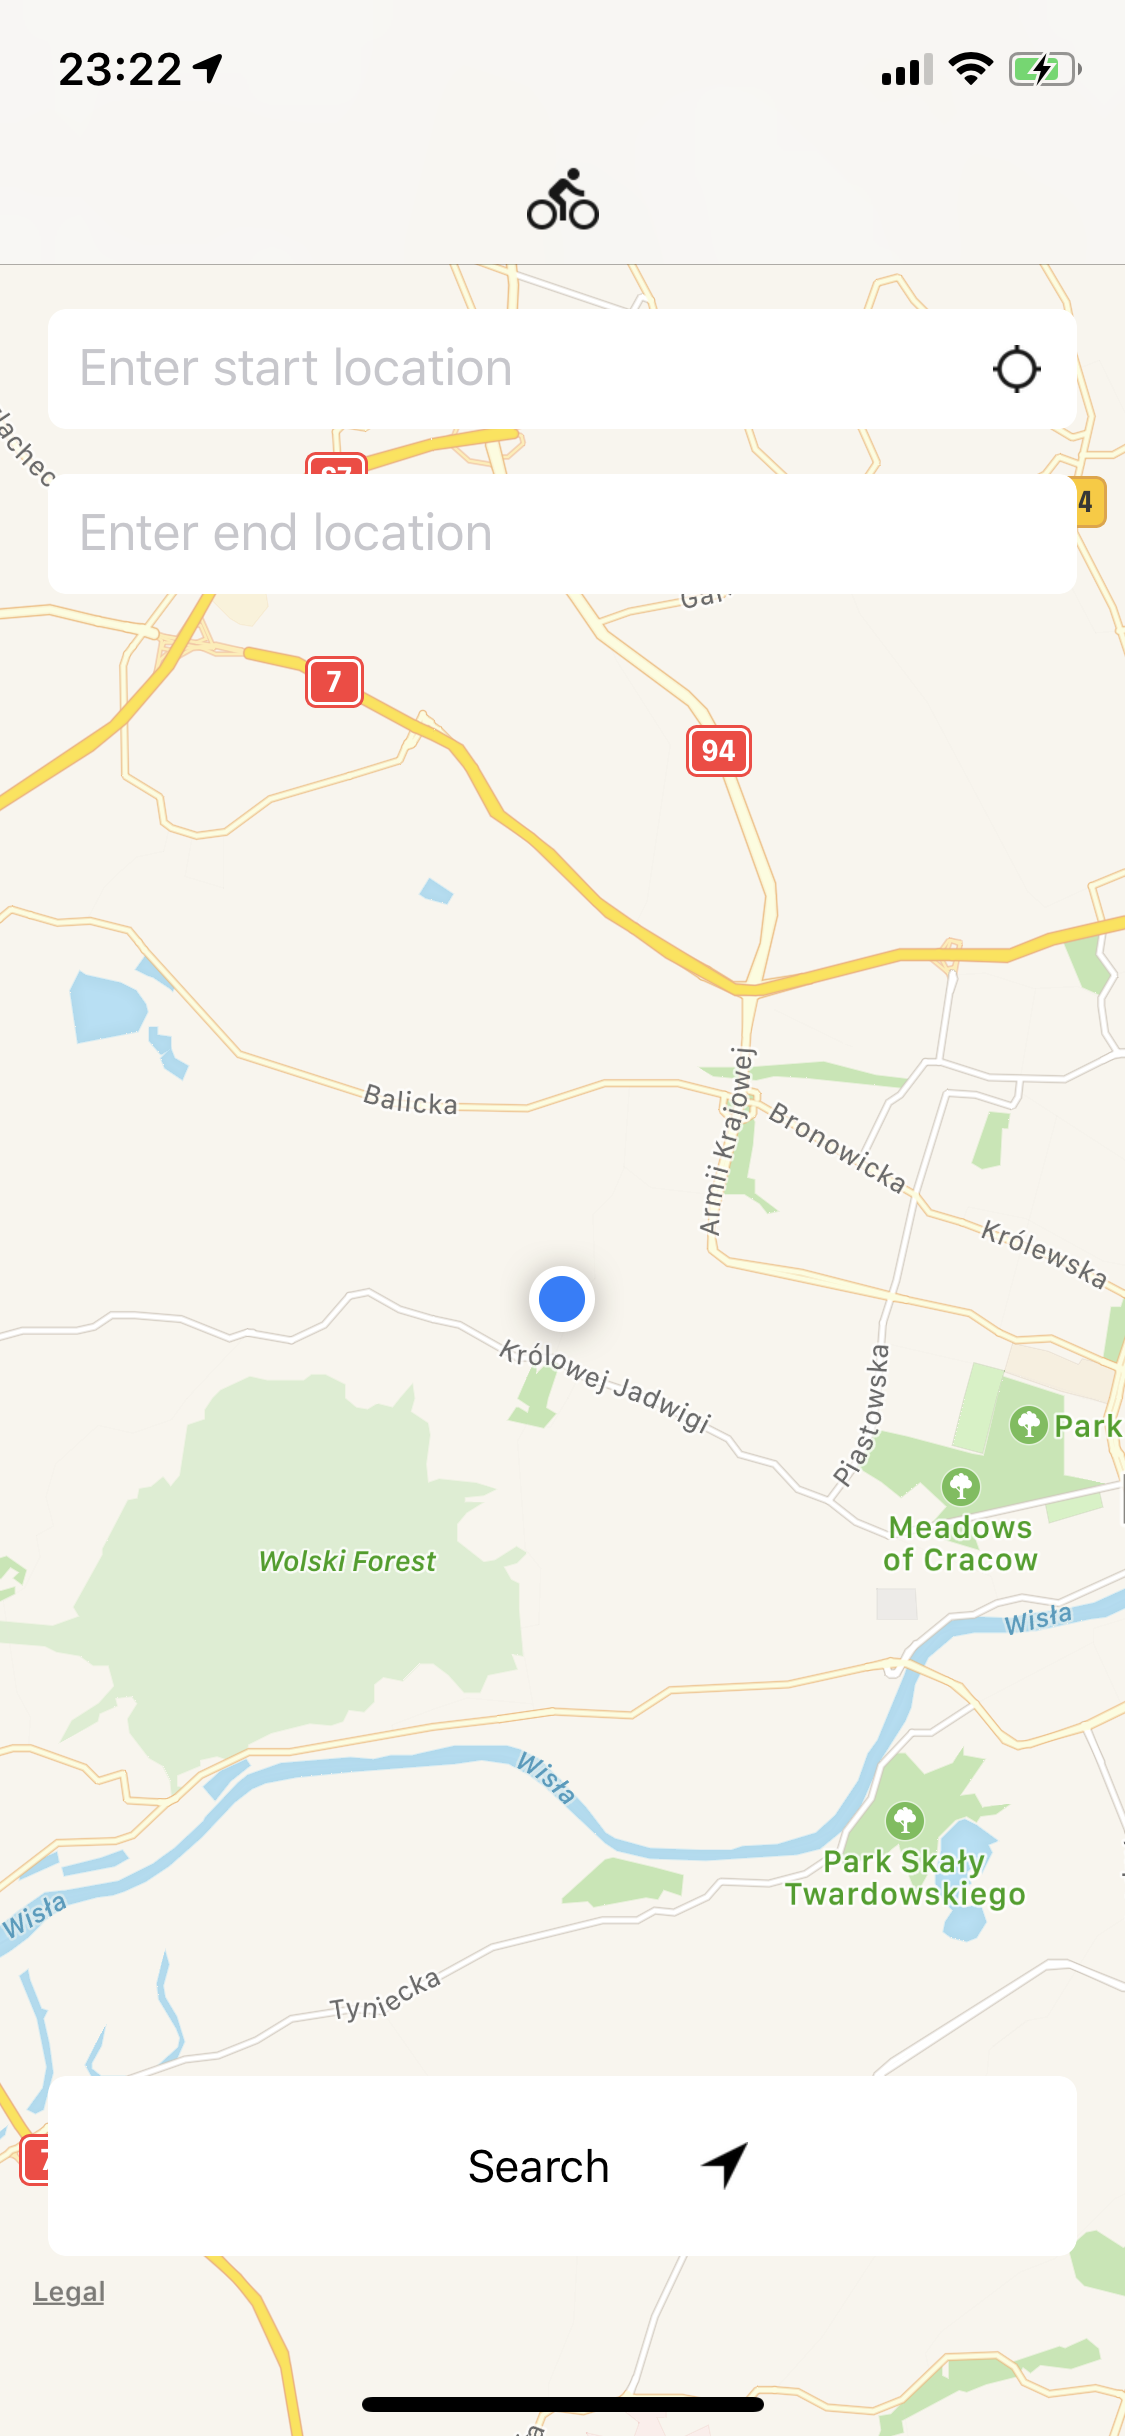
\includegraphics[height=12cm]{navi_initial}
\end{center}

Po wprowadzeniu punktów końcowych trasy, następuje jej wyszukanie, w tym celu aplikacji przygotowuje zapytanie pod endpoint „findOptimized” przekazując dane wpisane w polach tekstowych, a na czas ładowania odpowiedzi wyświetla indykator ładowania na górnym panelu oraz blokuje interakcje użytkownika ze wszystkimi elementami interfejsu użytkownika poza mapą. Po pobraniu trasy jest ona przekształcana na modele po stronie aplikacji oraz rysowana na mapie. Linią ciągłą zaznaczona jest trasa, linią przerywaną odcinki poza trasowe które trzeba pokonać aby dostać się z aktualnej lokalizacji użytkownika do początku trasy oraz z końca trasy do punktu końcowego wprowadzonego przez użytkownika. W celu odpowiedniej wizualizacji, po narysowaniu mapa jest odpowiednio przybliżana aby pokazać użytkownikowi przebieg całej trasy od jej początku do końca. Ekran z narysowaną mapą przedstawiono na poniższej ilustracji.

\begin{center}
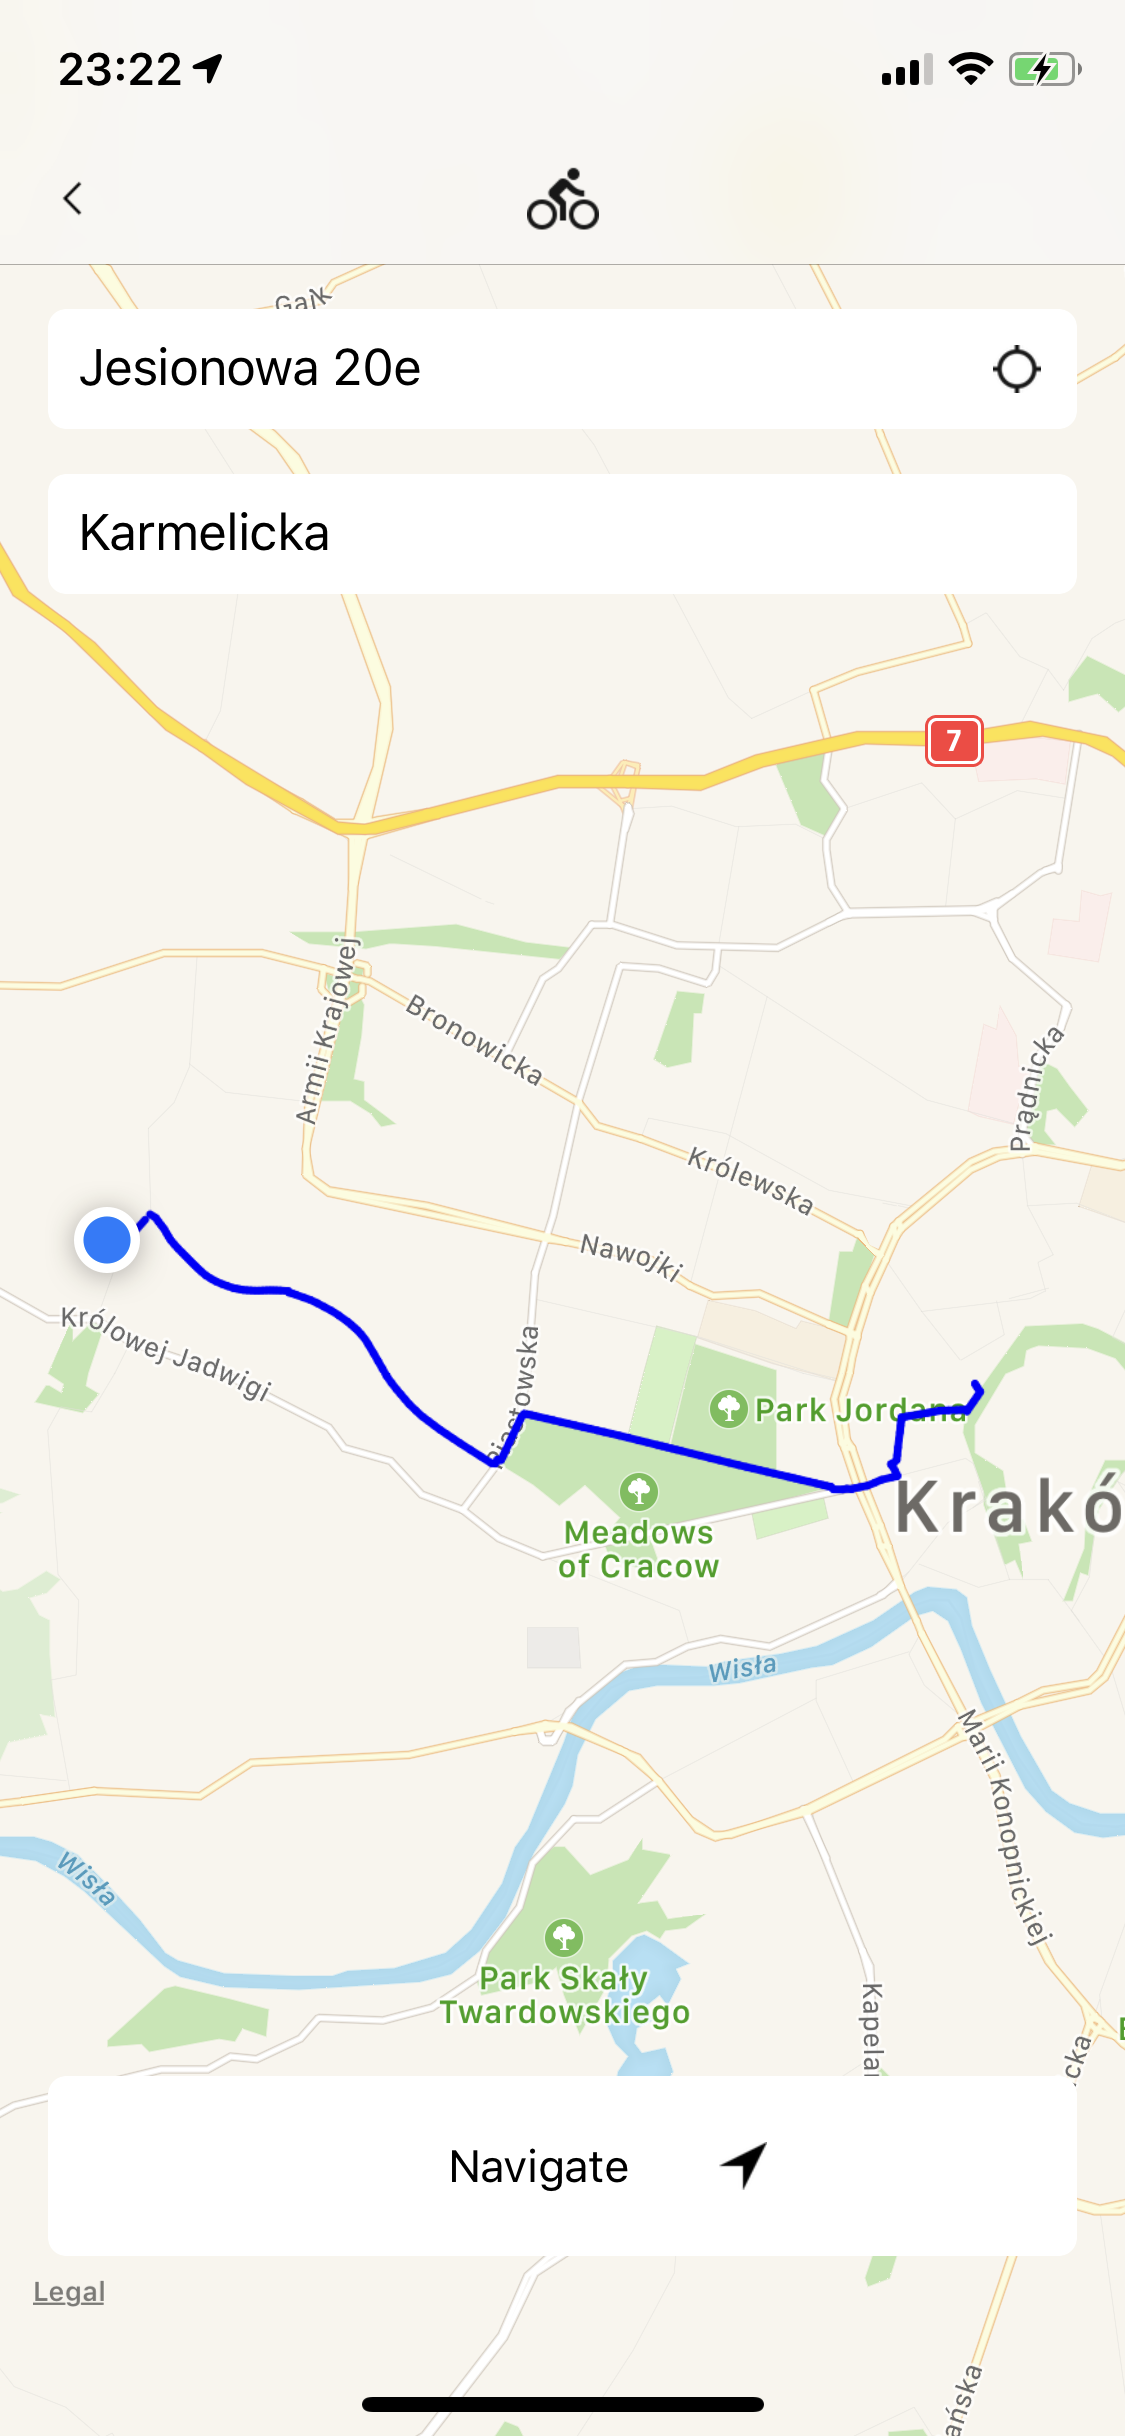
\includegraphics[height=12cm]{navi_route_marked}
\end{center}

Po wciśnięciu przycisku nawiguj zostaje włączony proces nawigacji użytkownika po trasie. W pierwszej fazie jest to prowadzenie do początku trasy, mapa zostaje odpowiednio przybliżona aby objąć trasę z punktu początkowego na początek trasy, lokalizacja użytkownika jest przedstawiona w postaci standardowego punkty na mapie obsługiwanego przez bibliotekę MapKit.

\begin{center}
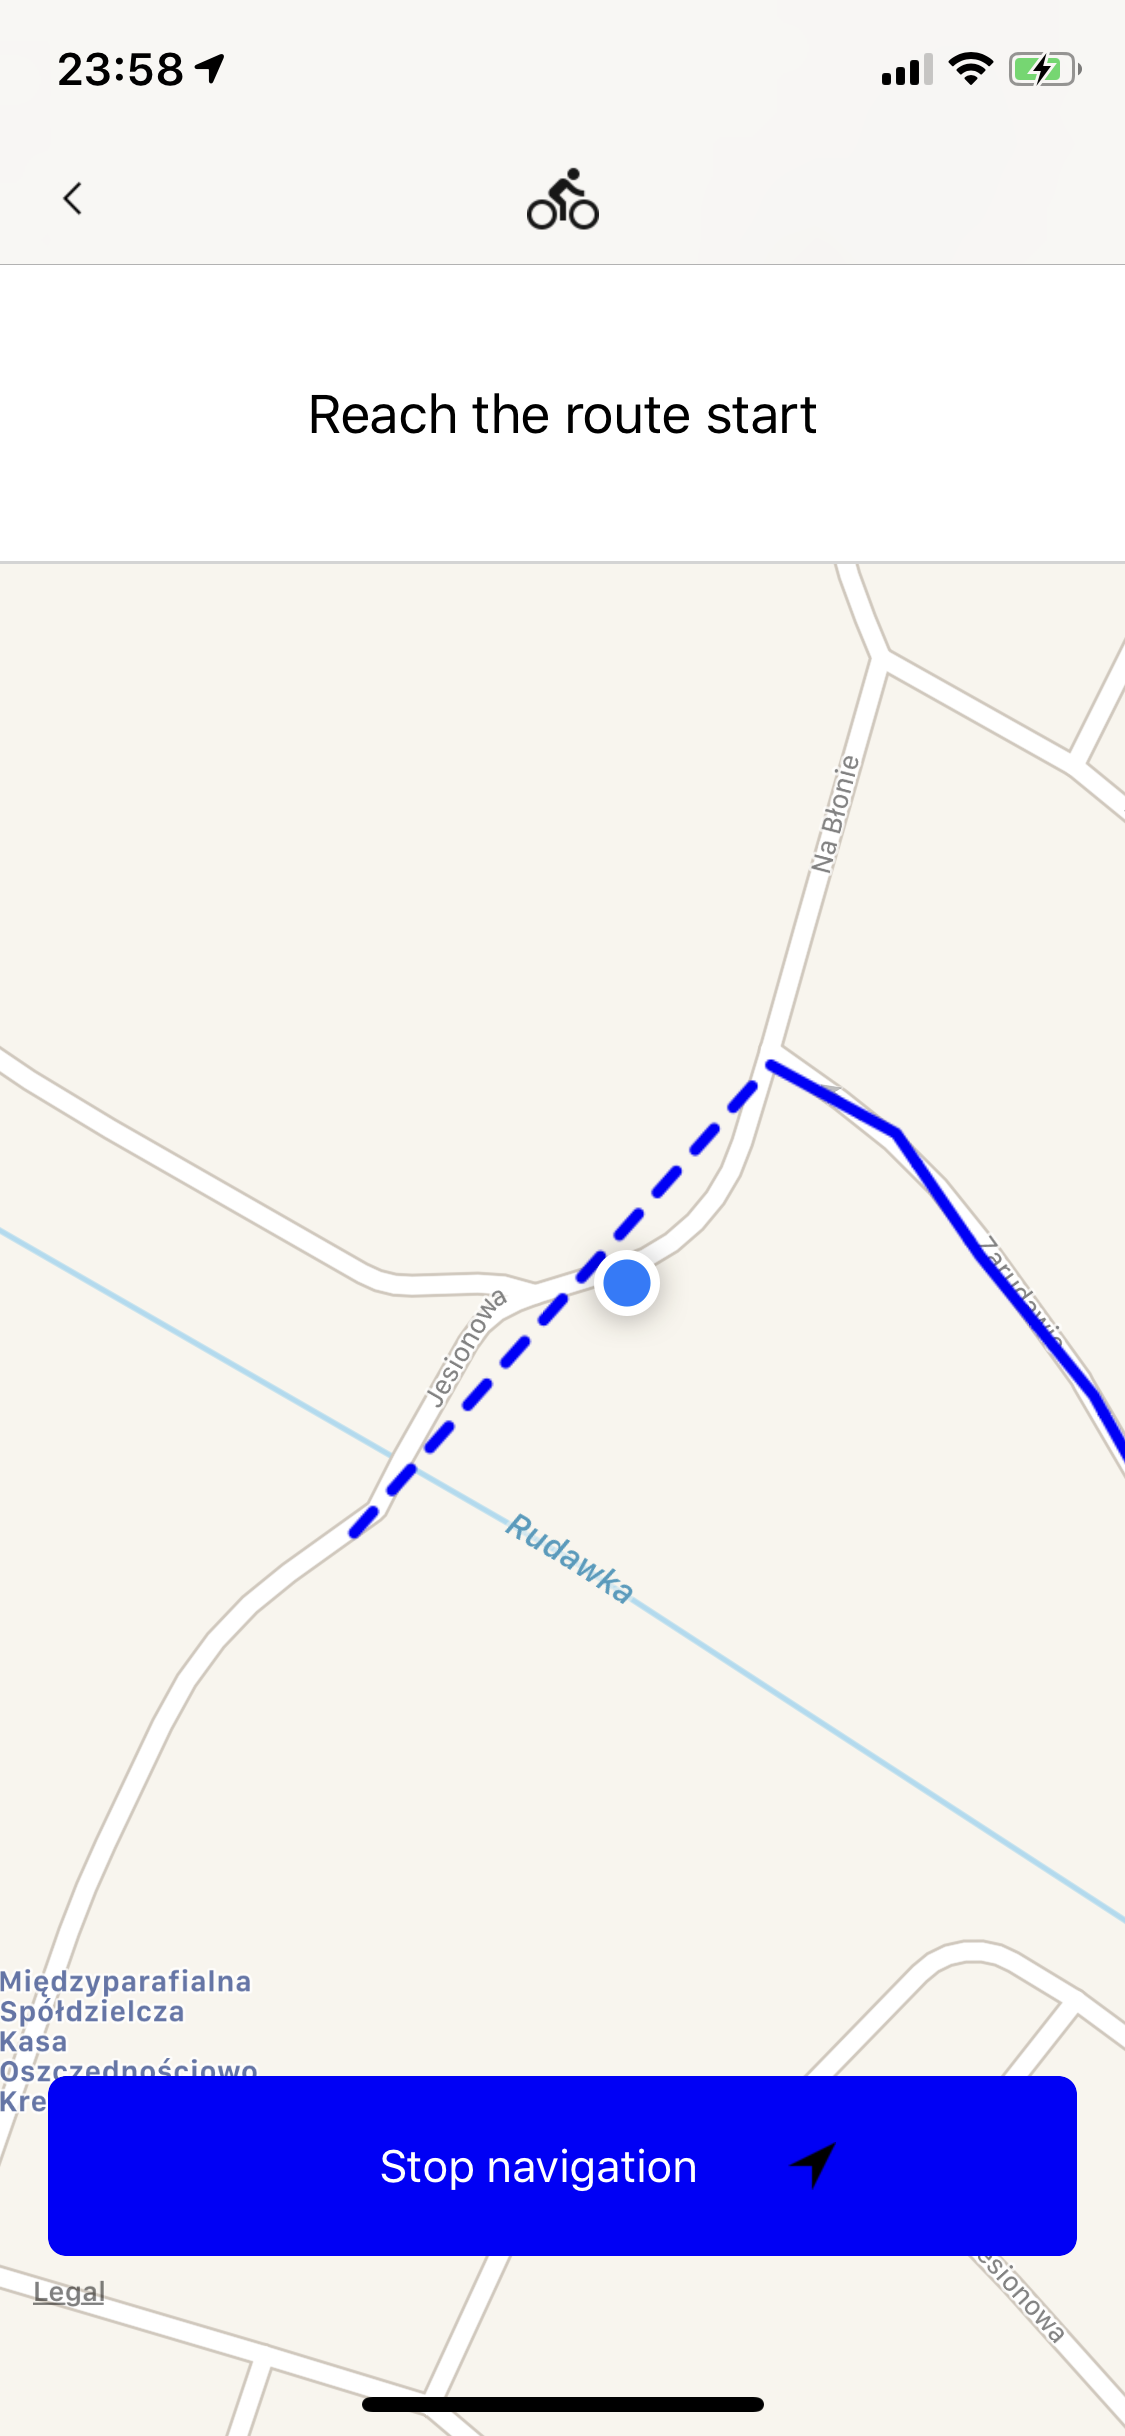
\includegraphics[height=12cm]{navi_reach_start}
\end{center}

Po dojściu użytkownika w obręb wyznaczonej trasy, interfejs użytkownika rozpoczyna nawigowanie go po trasie. Punkt wyznaczający aktualną lokalizację jest co sekundę animowanie przesuwany na pozycję na trasie odpowiadającą najbliższemu segmentowi w stosunku do rzeczywistej pozycji użytkownika na mapie. W przypadku wykrycia przez aplikację zakrętu w obrębie około najbliższych 200 metrów, na górnym panelu jest wyświetlana wskazówka zawierająca kierunek zakrętu oraz aktualną odległość po której wystąpi. W przypadku gdy użytkownik zjedzie z trasy, na górnym panelu jest przedstawiona instrukcja sugerująca powrót na trasę, zaś gdy oddali się od niej za daleko, instrukcja zmienia się w informację o wyznaczaniu nowej trasy do punktu końcowego.

\begin{center}
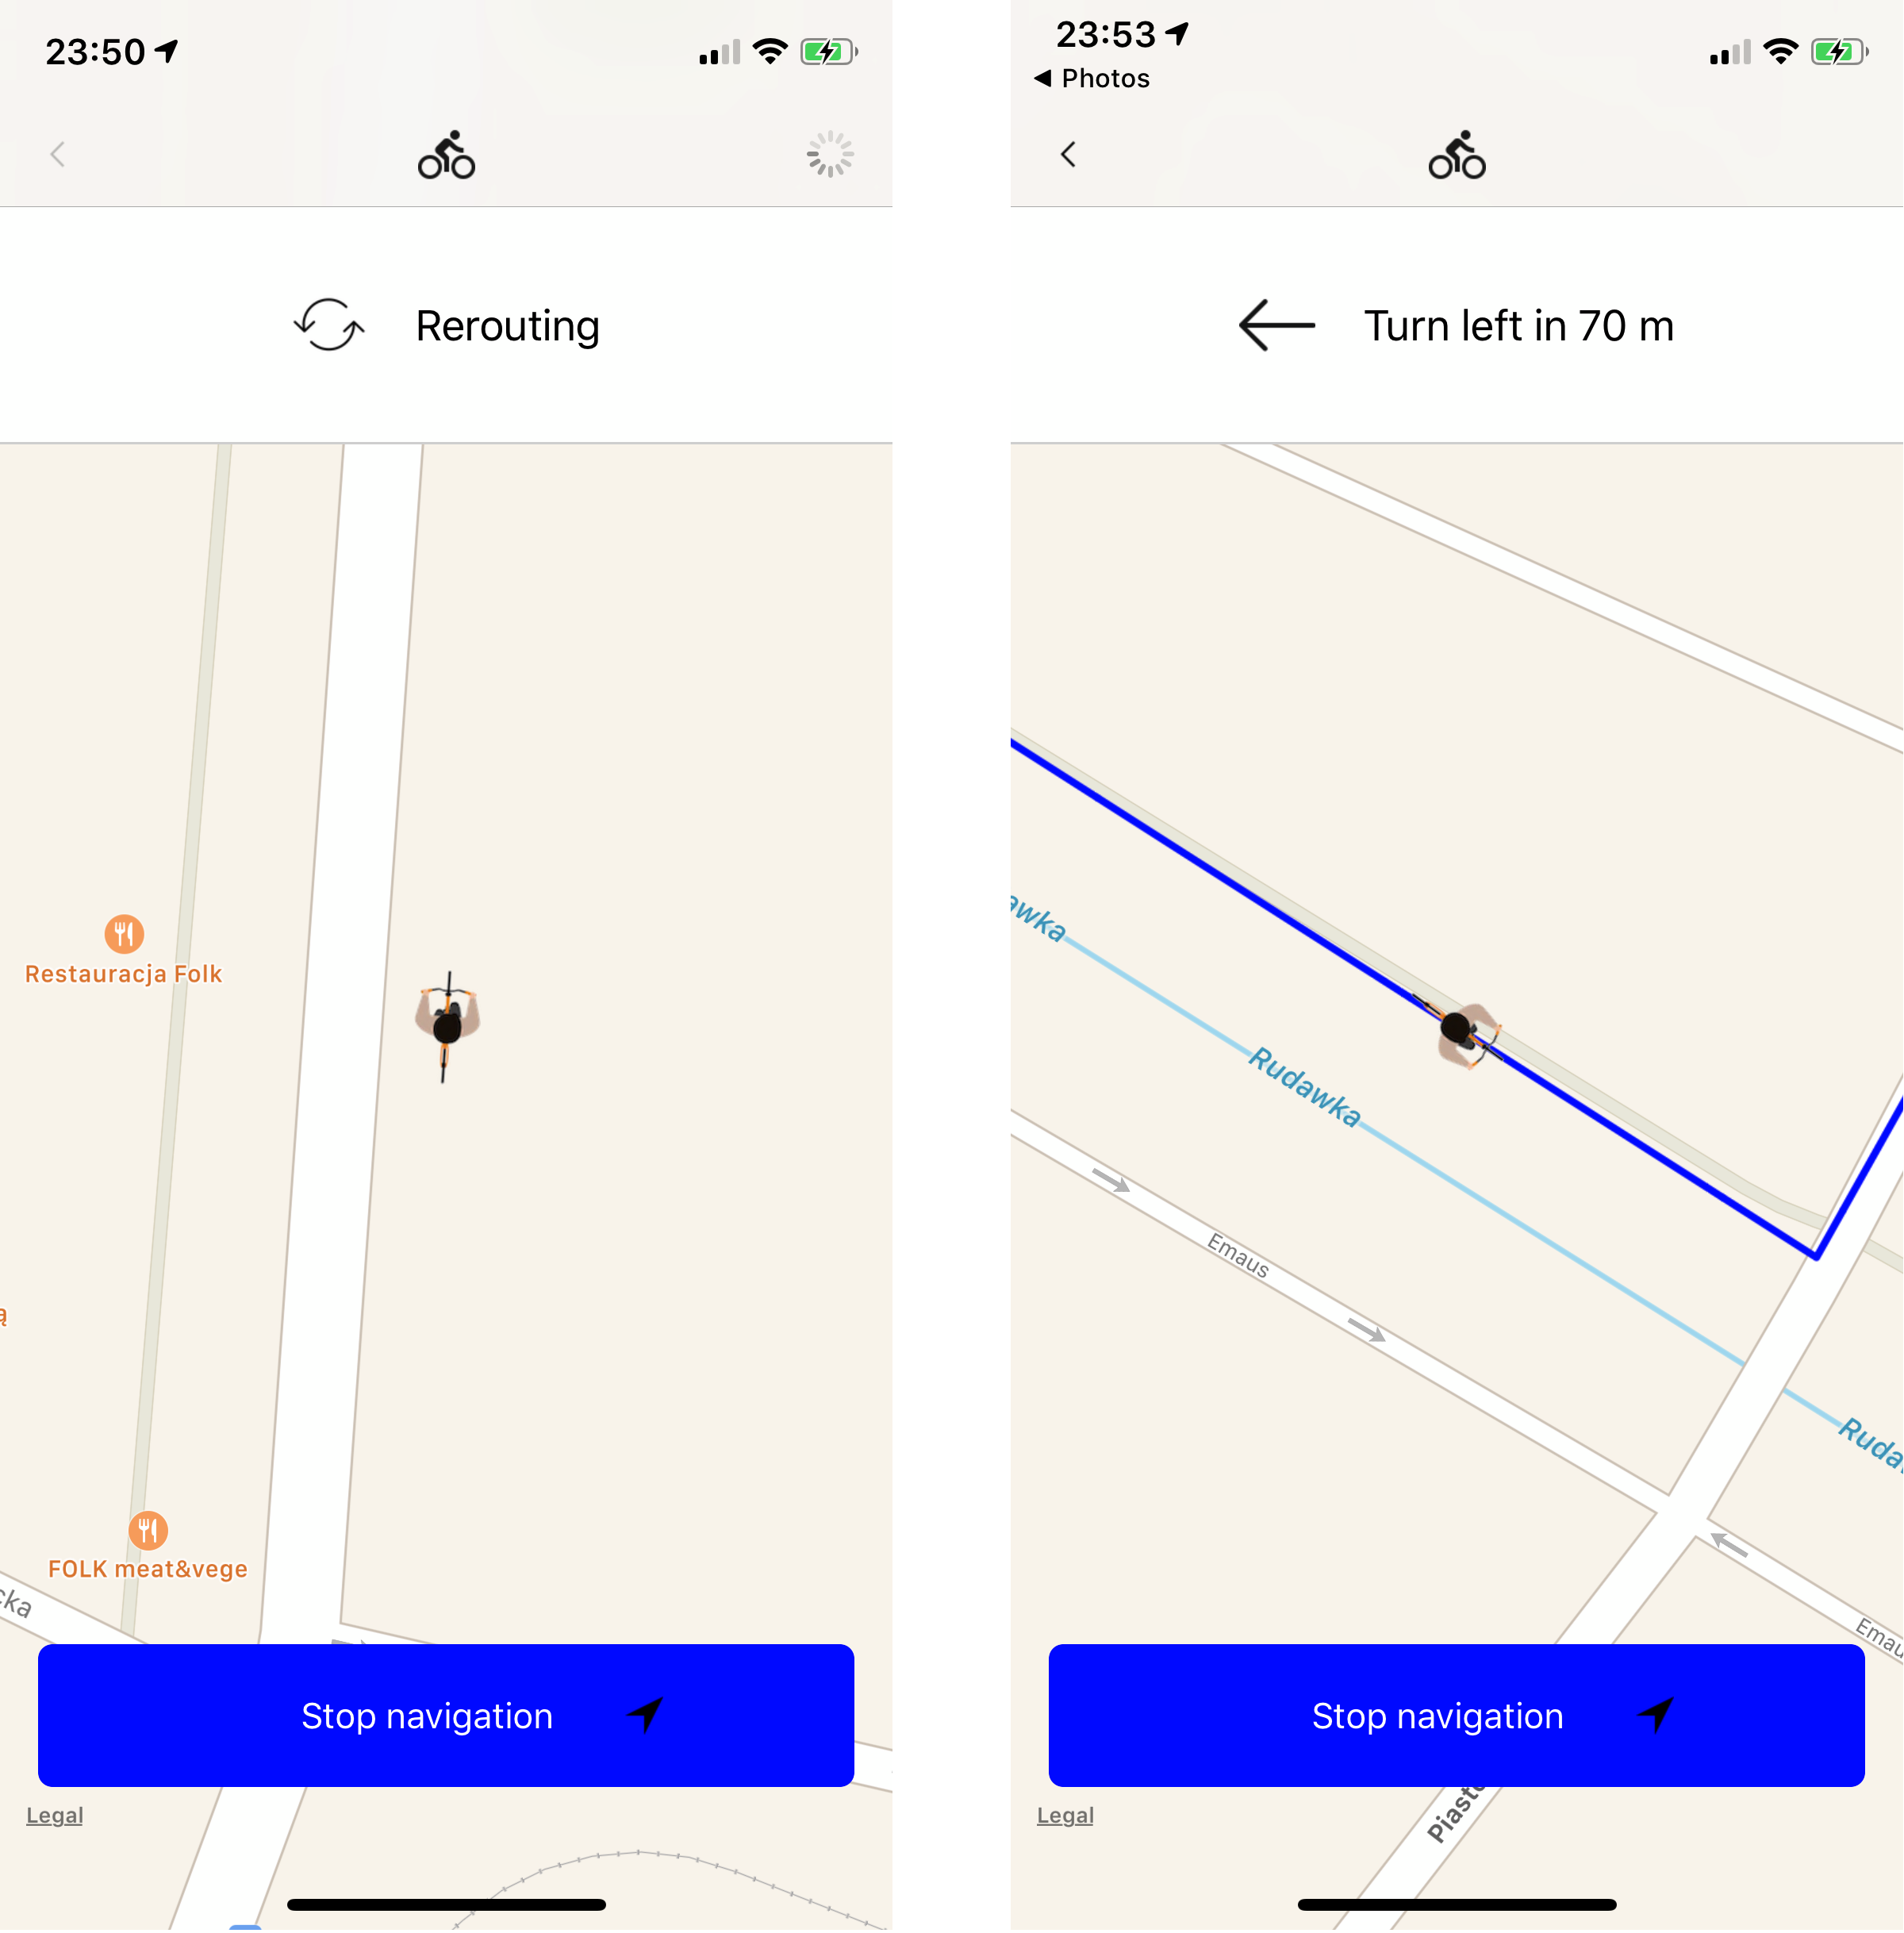
\includegraphics[height=12cm]{navi_guidance}
\end{center}

\subsection{Opis działania nawigacji}

System nawigacji w aplikacji został zaimplementowany w celu wizualizacji aktualnej lokalizacji użytkownika w stosunku do trasy która została wyznaczona. Działanie systemu składa się z zestawu stanów pomiędzy którymi algorytm może przechodzić w przypadku wykrycia określonych warunków. W poniższym akapicie została przedstawiona lista stanów na które składa się proces nawigacji a także dokładny opis warunków koniecznych do przejścia pomiędzy nimi. W celu wizualizacji procesu został także stworzony diagram stanów odwzorowujący cały proces.

Lista stanów w których może znaleźć się proces nawigacji użytkownika:

\begin{itemize}
\item Dojście z aktualnej lokalizacji do punktu startowego trasy
\item Nawigacja użytkownika po trasie
\item Dojście z końca trasy do punktu końcowego nawigacji
\item Zejście z trasy - w przypadku gdy użytkownik znalazł się więcej niż 30m ale nie więcej niż 150m od trasy.
\item Potrzeba wyznaczenia nowej trasy - gdy użytkownik znalazł się dalej niż 150m od najbliższego segmentu trasy.
\end{itemize}

W momencie gdy użytkownik rozpoczyna nawigację, zostaje włączony proces który co sekundę pobiera aktualną lokalizację użytkownika z klienta lokalizacji i wyznacza aktualny stan aplikacji. Startowym stanem jest prowadzenie użytkownika do początku trasy. Jako że pokrycie Krakowa ścieżkami rowerowymi oraz drogami z niskim ograniczenie prędkości jest względnie małe, w większości przypadków użytkownik na początku będzie musiał przemieścić się kilkaset metrów poza trasami wspieranymi przez aplikację. W tym celu jest rysowana prosta linia pomiędzy punktem początkowym, wpisanym przez użytkownika, a początkiem trasy a mapa jest odpowiednio przybliżana aby umożliwić użytkownikowi proste dotarcie na drogę. \newline
W czasie fazy prowadzenia użytkownika na start trasy, co każdy cykl odświeżenia aktualnego stanu, jest sprawdzane czy użytkownik znalazł się w otoczeniu 10 metrów w stosunku do początku któregokolwiek z segmentów składających się na trasę. Sprawdzanie jedynie segmentu będącego punktem początkowym trasy nie daje w tym wypadku oczekiwanego rezultatu ze względu na częste błędy w wyznaczeniu pozycji użytkownika przez moduł GPS a także przez fakt że często na trasę wjeżdżamy nie dokładnie w punkcie jej początku a przykładowo dopiero po pierwszych stu metrach. Posiadając dostępny zbiór danych aplikacja nie jest w stanie niestety wyznaczyć optymalnej trasy użytkownika pomiędzy jego aktualnym położeniem a punktem końcowym trasy. Jesteśmy w stanie jedynie oszacować że najbardziej prawdopodobnym punktem będzie najbliższy wierzchołek grafu zakładając ich odpowiednią granulację otrzymaną podczas procesy jego tworzenia. \newline
W przypadku wykrycia wejścia użytkownika w obręb wyznaczonej dla niego trasy aplikacja przechodzi w stan nawigowania po trasie. Aby uniknąć błędów w wyznaczaniu pozycji użytkownika i prowadzenia go 10-20 metrów obok zaznaczonej drogi, został zaimplementowany mechanizm dociągania do wyznaczonej ścieżki. W tym celu w każdym kroku filtrowane są wszystkie drogi w celu znalezienia tej znajdującej się najbliżej użytkownika, zastosowano do tego porównanie sumy odległości od początków z każdej tych dróg, podzielonej przez jej długość. Dzięki temu rozwiązaniu algorytm wyeliminował znajdywanie jedynie krótkich dróg dla których suma odległości do początku oraz do końca była najmniejsza. \newline
Po odnalezieniu najbliższej drogi, algorytm przeszukuje wszystkie jej segmenty w celu znalezienia tego znajdującego się najbliżej. Jako że długości segmentów zostały ujednolicone w jednym z kroków tworzenia grafu, na tym etapie możemy zastosować prostsze porównanie które sprawdza jedynie sumę odległości użytkownika od początku oraz końca każdego z segmentów.
W następnym kroku, uzyskany segment zostaje podzielony na 20 równych sobie odcinków, najbliższy aktualnej pozycji użytkownika zostaje przypisany jako najbardziej odpowiedni a aplikacja sztucznie dociąga lokalizację użytkownika do tego właśnie punktu. \newline
Powyżej opisana metoda działa w przypadku gdy wyznaczona pozycja użytkownika znajduje się nie dalej niż 50 metrów od trasy. W przypadku gdy użytkownik znajdzie się w odległości większej niż 50 metrów, algorytm przestaje zwracać pozycję użytkownika dociągniętą do trasy a zamiast tego zwraca rzeczywiste położenie użytkownika na mapie. Ten tryb został zaimplementowany w celu pokazania użytkownikowi informacji że znalazł się poza trasą i powinien na nią wrócić. Ogranicza to także niepotrzebne zapytania do strony serwerowej w przypadku gdy użytkownik celowo zszedł z trasy aby na przykład wejść do sklepu.
W przypadku gdy wykryte położenie znajduje się dalej niż 150m od trasy zaznaczonej na mapie, algorytm zakłada że należy dla użytkownika wyznaczyć nową trasę, o czym informuje przez wysłanie określonego sygnału oraz zakończenie działania. W tym momencie zostaje wysłane zapytanie do serwera o nową trasę zawierające aktualną pozycję użytkownika oraz miejsce docelowe określone na początku procesu nawigacji. W przypadku gdy zapytanie się powiedzie, algorytm zostaje zrestartowany i wraca do stanu początkowego, czyli prowadzenia użytkownika do początku trasy.
W każdym kroku działania algorytmu jest także sprawdzana odległość aktualnej pozycji użytkownika w stosunku do końca wyznaczonej trasy. Jeśli ta jest mniejsza niż 50 metrów, zakładamy że użytkownik dotarł do końca i nawigacja przechodzi w tryb prowadzenia użytkownika do punktu końcowego trasy, pokazując jednocześnie odpowiednio przybliżony obszar na mapie. W tym kroku założona odległość od punktu końcowego musi być znacznie większa niż ta która stanowi o momencie wejścia na trasę ponieważ użytkownik może znajdywać się w najbliższym otoczeniu punktu końcowego jedynie przez krótką chwilę.


\subsection{Opis testów}

Do testów działania nawigacji zostały wykorzystane pliki GPX(GPS Exchange Format) które, sformatowane w odpowiedni sposób umożliwiają symulację lokalizacji użytkownika zarówno przy użyciu symulatora jak i na rzeczywistym urządzeniu z systemem iOS. Plik GPX jest to plik w formacie XML który składa się. Ze zbioru punktów oraz czasów skorelowanych z każdym z punktów. System odczytując ten plik animuje lokalizację użytkownika tak aby przeszła pomiędzy wszystkimi określonymi punktami w ściśle wyznaczonym czasie. Do stworzenia plików użyto strony http://www.gpsies.com/createTrack.do która udostępnia graficzny interfejs do zaznaczania punktów na mapie oraz określenia z jaką prędkością chcielibyśmy aby użytkownik się pomiędzy nimi przemieszczał. Pobrany stamtąd plik następnie trzeba poddać obróbce w postaci usunięcia kilku linii aby był wspierany przez symulację lokalizacji w systemie iOS.

\section{Opis stworzonej strony internetowej}

\subsection{Opis technologii i użytych bibliotek}

W ramach projektu została zaimplementowana także strona internetowa, która w intuicyjny sposób pozwala użytkownikowi wyszukać trasę pomiędzy wpisanymi adresami oraz wyświetla ją na mapie. 
Aplikacja została stworzona w oparciu o bibliotekę ReactJS która pozwala w szybki sposób zbudować prototyp strony internetowej przy użyciu języka Javascript oraz predefiniowanych elementów strony takich jak przyciski czy pola tekstowe. Do wyświetlenia map użyto map udostępnionych przez openstreetmap przez bibliotekę React Leaflet. Leaflet jest to biblioteka umożliwiająca bardzo proste renderowanie map przy użyciu Javascript, React Leaflet dodaje do tego mapy w postacie gotowych komponentów React. Wybór został podyktowany faktem, że prostsze w użyciu i wydajniejsze mapy Google w celu wyświetlenia przy użyciu języka Javascript wymagają płatnej subskrybcji.
W projekcie strony internetowej, do zarządzania zewnętrznymi zależnościami użyto programu yarn, a do zapytań http użyto biblioteki axios. Narzędzia te nie różnią się od tych dla aplikacji serwerowej, dlatego też w tym akapicie pominięto ich opis.

\subsection{Spis ekranów, opis działania}

Aplikacja jest bardzo prosta, składa się z dwóch ekranów. Na pierwszym z nich są przedstawione dwa pola tekstowe oraz przycisk umożliwiający wyszukanie trasy, jego wygląd przedstawiono na poniższej ilustracji.

\begin{center}
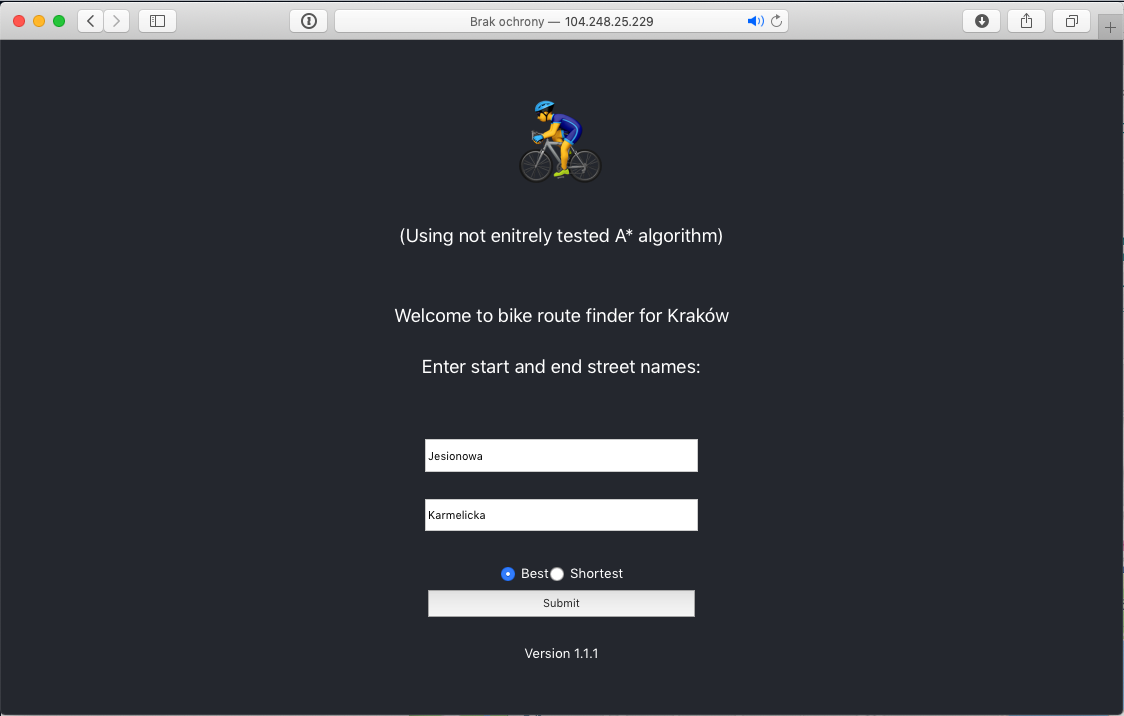
\includegraphics[width=\textwidth]{web_form}
\end{center}

Kolejny z ekranów ma zaimplementowaną logikę pobierania trasy w zależności od stanu przekazanego do niego z ekranu wpisywania danych. Wykorzystując bibliotekę axios wykonuje zapytanie pod endpoint „visualizationPoints” zawierając w kwerendzie wymagane dane. Zwrócona odpowiedź w formacie JSON zawiera zbiór wszystkich punktów na mapie który należy ze sobą połączyć aby przestawić użytkownikowi wizualizację wyznaczonej ścieżki. Ścieżka jest przedstawiona na mapie obejmującej całość ekranu.

\begin{center}
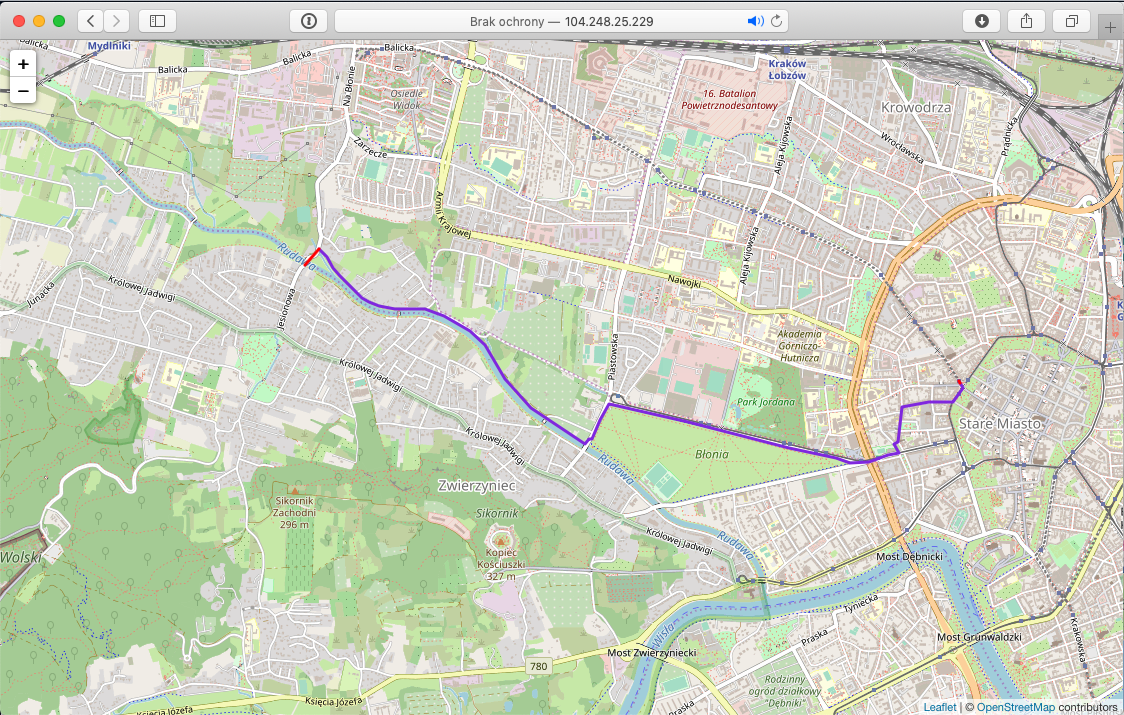
\includegraphics[width=\textwidth]{web_map}
\end{center}
\chapter{Analiza otrzymanych wyników}
\label{cha:analiza_otrzymanych_wynikow}


\section{Analiza działania użytych algorytmów}

W celu implementacji algorytmu wyszukania optymalnych tras, w aplikacji została zaimplementowana obsługa kilku algorytmów wyszukiwania ścieżek w grafie. Standardowo aplikacja korzysta tylko z jednego z nich, implementacja ma na celu tylko ich porównanie. W poniższych akapitach przedstawiono testy porównawcze prędkości działania algorytmów podczas wyznaczania tras pomiędzy zestawem wybranych losowo punktów na mapie Krakowa. 
W celu heterogenizacji wyznaczonych tras, punkty początkowe i końcowe każdej z nich zostały dobrane w taki sposób, aby pokryły odpowiedni obszar Krakowa, a także przebiegały w miejscach, gdzie znajduje się zarówno dużo, jak i mało ścieżek zawartych w posiadanym zbiorze danych. Z tego powodu niektóre z nich przebiegają w okolicach rynku, a inne przez Wolę Justowską, gdzie jedyną ścieżką w posiadanym zbiorze jest droga po wale rzeki Rudawy.
Obydwa z zaimplementowanych algorytmów gwarantują każdorazowo wyznaczenie optymalnej trasy. Nie kończą one przeszukiwania po uzyskaniu pierwszej znalezionej trasy, stąd porównanie można uznać za miarodajny wynik złożoności obliczeniowej każdego z algorytmów.

\subsection{Porównanie działania algorytmu z wykorzystaniem algorytmu Dijkstra i A*}

Na poniższym wykresie zestawiono czasy działania obydwu algorytmów wraz z opisem trasy, dla której każdy z czasów został wyznaczony.

\begin{figure}[H]
\centering
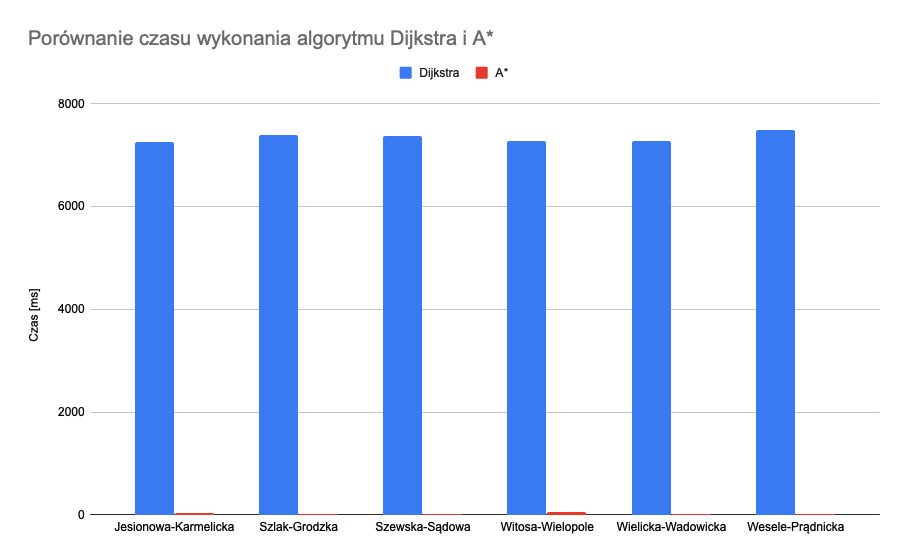
\includegraphics[width=0.7\textwidth]{czas_dijkstra_vs_a}
\caption{Czasy wykonania algorytmu Dijkstra i A* dla wybranych danych testowych.}
\end{figure}

Z wykresu można odczytać, że algorytm A* sprawdza się nieporównywalnie lepiej w stosunku do algorytmu Dijkstra w kontekście czasu wykonania. Z wykresu niełatwo jest nawet odczytać różnice w czasie działania ze względu na minimalny wkład czasów osiągniętych przez A*. W najgorszym z zaprezentowanych przypadków jego działanie było około 200-krotnie szybsze, zaś w najlepszym z przypadków różnica w prędkości działania była prawie 500-krotna. Z powyższego zestawienia jasno wynika, że do produkcyjnego zastosowania w aplikacji, w porównaniu z algorytmem Dijkstra, nadaje się tylko algorytm A*. Jest on za to znacznie bardziej czasochłonny w implementacji, stąd jego zastosowanie do zdecydowanie mniej złożonych grafów może być korzystniejsze. W celu zminimalizowania czasu wykonywania algorytmu Dijkstra można było zastosować odpowiednie zmniejszenie grafu na podstawie filtracji wierzchołków, które znajdują się wewnątrz obszaru na mapie zawartego przez punkt końcowy i początkowy. Jednak ze względu na brak potrzeby optymalizacji i odpowiednią wizualizację różnic czasu działania zaniechano tej modyfikacji.
W przypadku przeszukiwania grafu, w którym wierzchołki mogą być określone jako punkty na mapie, algorytm A* jest zdecydowanie szybszy ze względu na prostotę wyznaczenia heurystyki. W tym wypadku przewidywanie czy droga zbliża się do końca może być określone przez wyznaczenie odległości pomiędzy kolejnym sprawdzanym wierzchołkiem a punktem końcowym trasy z wyjątkowo małą złożonością obliczeniową, nie wymagającą dodatkowych iteracji po wierzchołkach czy krawędziach grafu. Dzięki temu, w przeciwieństwie do algorytmu Dijkstra, A* nie prowadzi przeszukania całego grafu przed wyznaczeniem optymalnej ścieżki, a ogranicza się jedynie do przeszukania szeregu dróg które prowadzą pomiędzy punktem końcowym i początkowym. \newline

\subsection{Czas działania algorytmu A* i Dijkstra w zależności od długości trasy}

Na poniższych wykresach przedstawiono czas działania algorytmu A* i Dijkstra w zależności od obszaru objętego przeszukiwaniem. W tym celu, na terenie Krakowa, wyznaczono zestaw tras w zakresie od bardzo krótkich, obejmujących tylko kilkaset metrów, do takich, które obejmują teren całego Krakowa.

\begin{figure}[H]
\centering
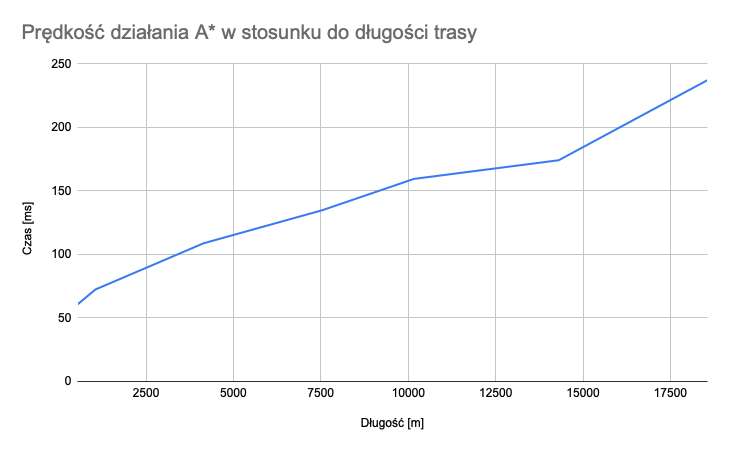
\includegraphics[width=0.7\textwidth]{a_a_dlugosc_trasy}
\caption{Czas wykonywania algorytmu A* w zależności od długości wyznaczonej trasy.}
\end{figure}

\begin{figure}[H]
\centering
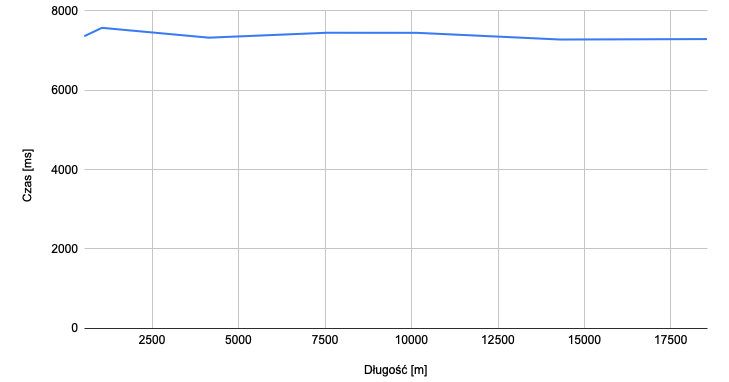
\includegraphics[width=0.7\textwidth]{dijkstra_a_dlugosc_trasy}
\caption{Czas wykonywania algorytmu Dijkstra w zależności od długości wyznaczonej trasy.}
\end{figure}

Z przedstawionych wykresów można odczytać, że czas działania algorytmu Dijkstra nie zależy od długości wyznaczonych tras. Delikatne fluktuacje czasu wykonania zależą od aktualnego użycia pamięci i procesora komputera podczas wykonywania testu. Jest to spowodowane zasadą działania algorytmu Dijkstra, który w każdym przypadku w pierwszej kolejności wykonuje obliczenia najkrótszych ścieżek pomiędzy wszystkimi wierzchołkami grafu.
Przeciwny przypadek obowiązuje dla algorytmu A*, który dzięki zastosowaniu heurystyki jest w stanie wykryć, gdy najkrótsza ścieżka została już odnaleziona i zatrzymać przeszukiwanie w odpowiednim przypadku. Z tego powodu w zależności od obszaru grafu obejmowanego przez przeszukanie, algorytm A* wykazuje znaczny, liniowy wzrost czasu wykonania.

\subsection{Porównanie algorytmu zachłannego A* i standardowej implementacji A*}

Kolejnym etapem analizy jest określenie czasu oraz jakości działania algorytmu zachłannego A* w stosunku do podstawowej wersji A*. W przeciwieństwie do standardowej implementacji, algorytm zachłanny, zyskując na czasie wykonania, nie gwarantuje wyznaczenia optymalnej ścieżki pomiędzy wierzchołkiem początkowym i końcowym. Bazując na przekazanej heurystyce, stara się wyznaczyć najlepsze lokalne rozwiązania podzbiorów składających się na wynikową trasę, następnie łączy uzyskane podzbiory w celu wyznaczenia trasy. W poniższych akapitach zawarto analizę czasu wykonania oraz wyznaczonych wag tras w zależności od typu algorytmu.

Na poniższym wykresie przedstawiono zestawienie wag tras wyznaczonych przez obydwa algorytmy dla uprzednio wyznaczonego zestawu dróg testowych.

\begin{figure}[H]
\centering
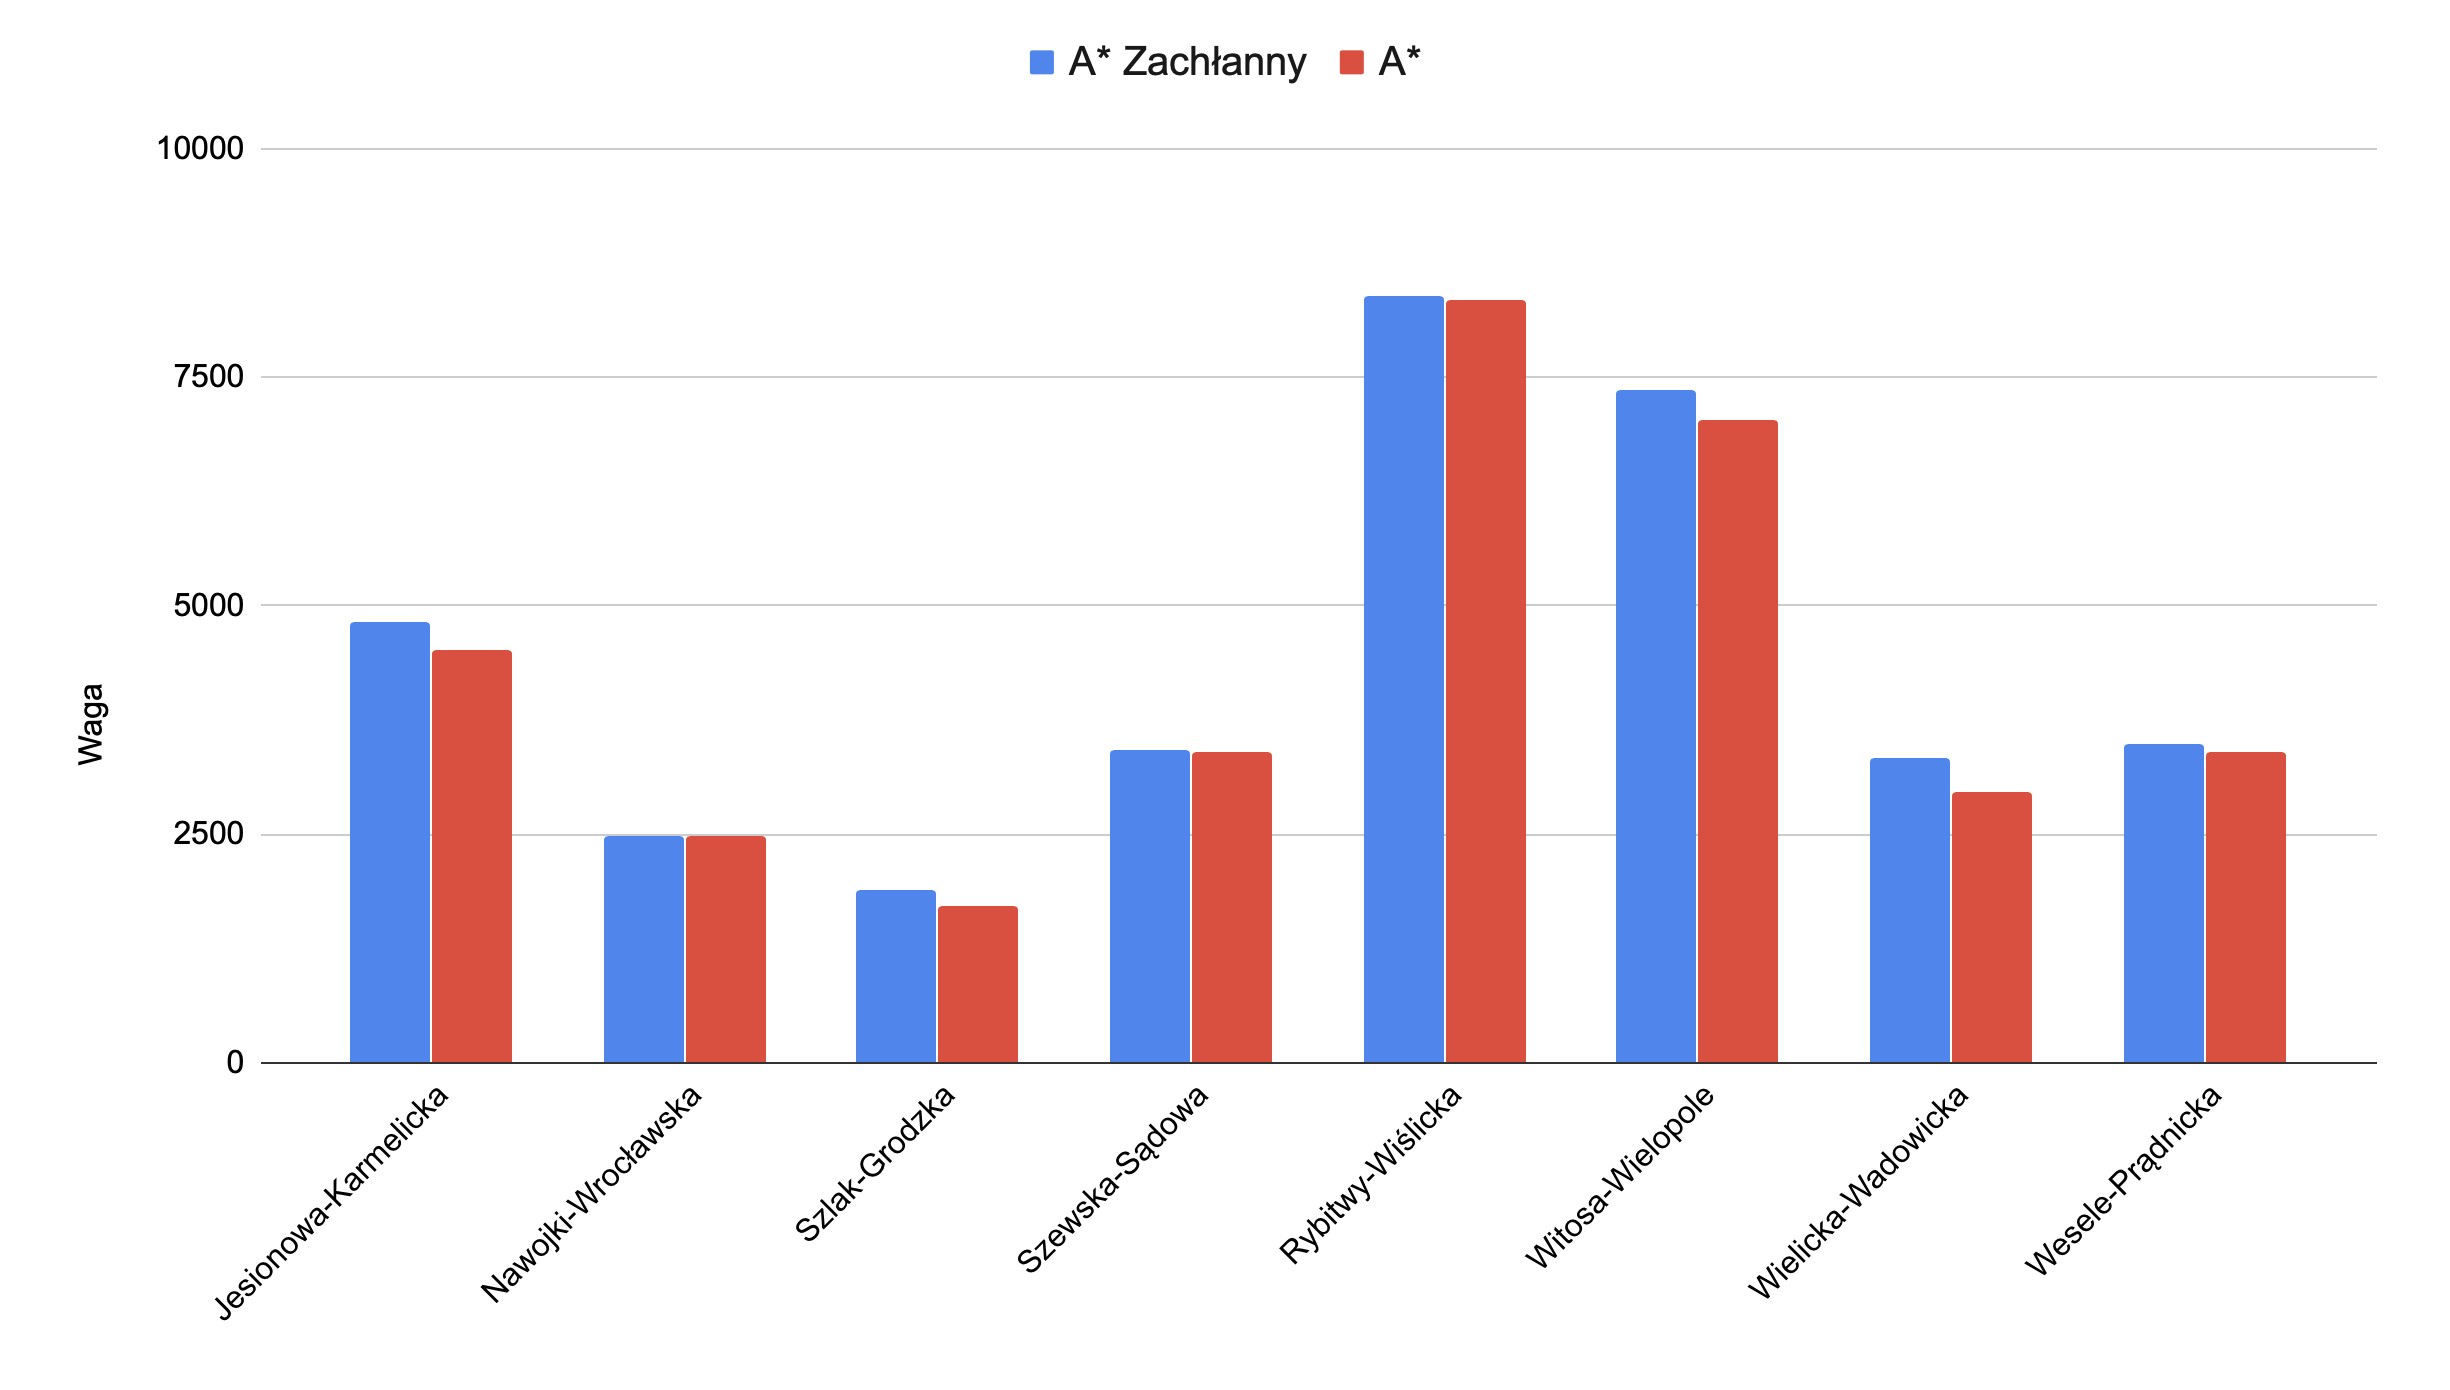
\includegraphics[width=0.7\textwidth]{waga_a_vs_a_greedy}
\caption{Zestawienie wag wyznaczonych przez algorytm A* oraz A* zachłanny dla wybranego zestawu danych testowych.}
\end{figure}

Korzystając z wartości przedstawionych na powyższym wykresie można odczytać, że poza przypadkiem bardzo krótkiej drogi pomiędzy ulicami Nawojki i Wrocławską, zachłanna odmiana algorytmu A* w każdym wypadku wyznaczyła trasę, która z punktu widzenia wagi jest gorsza niż ta wyznaczona przez standardową odmianę algorytmu A*.

Na poniższym wykresie przedstawiono zestawienie czasu działania dla uprzednio wyznaczonego zestawu testowych ścieżek.

\begin{figure}[H]
\centering
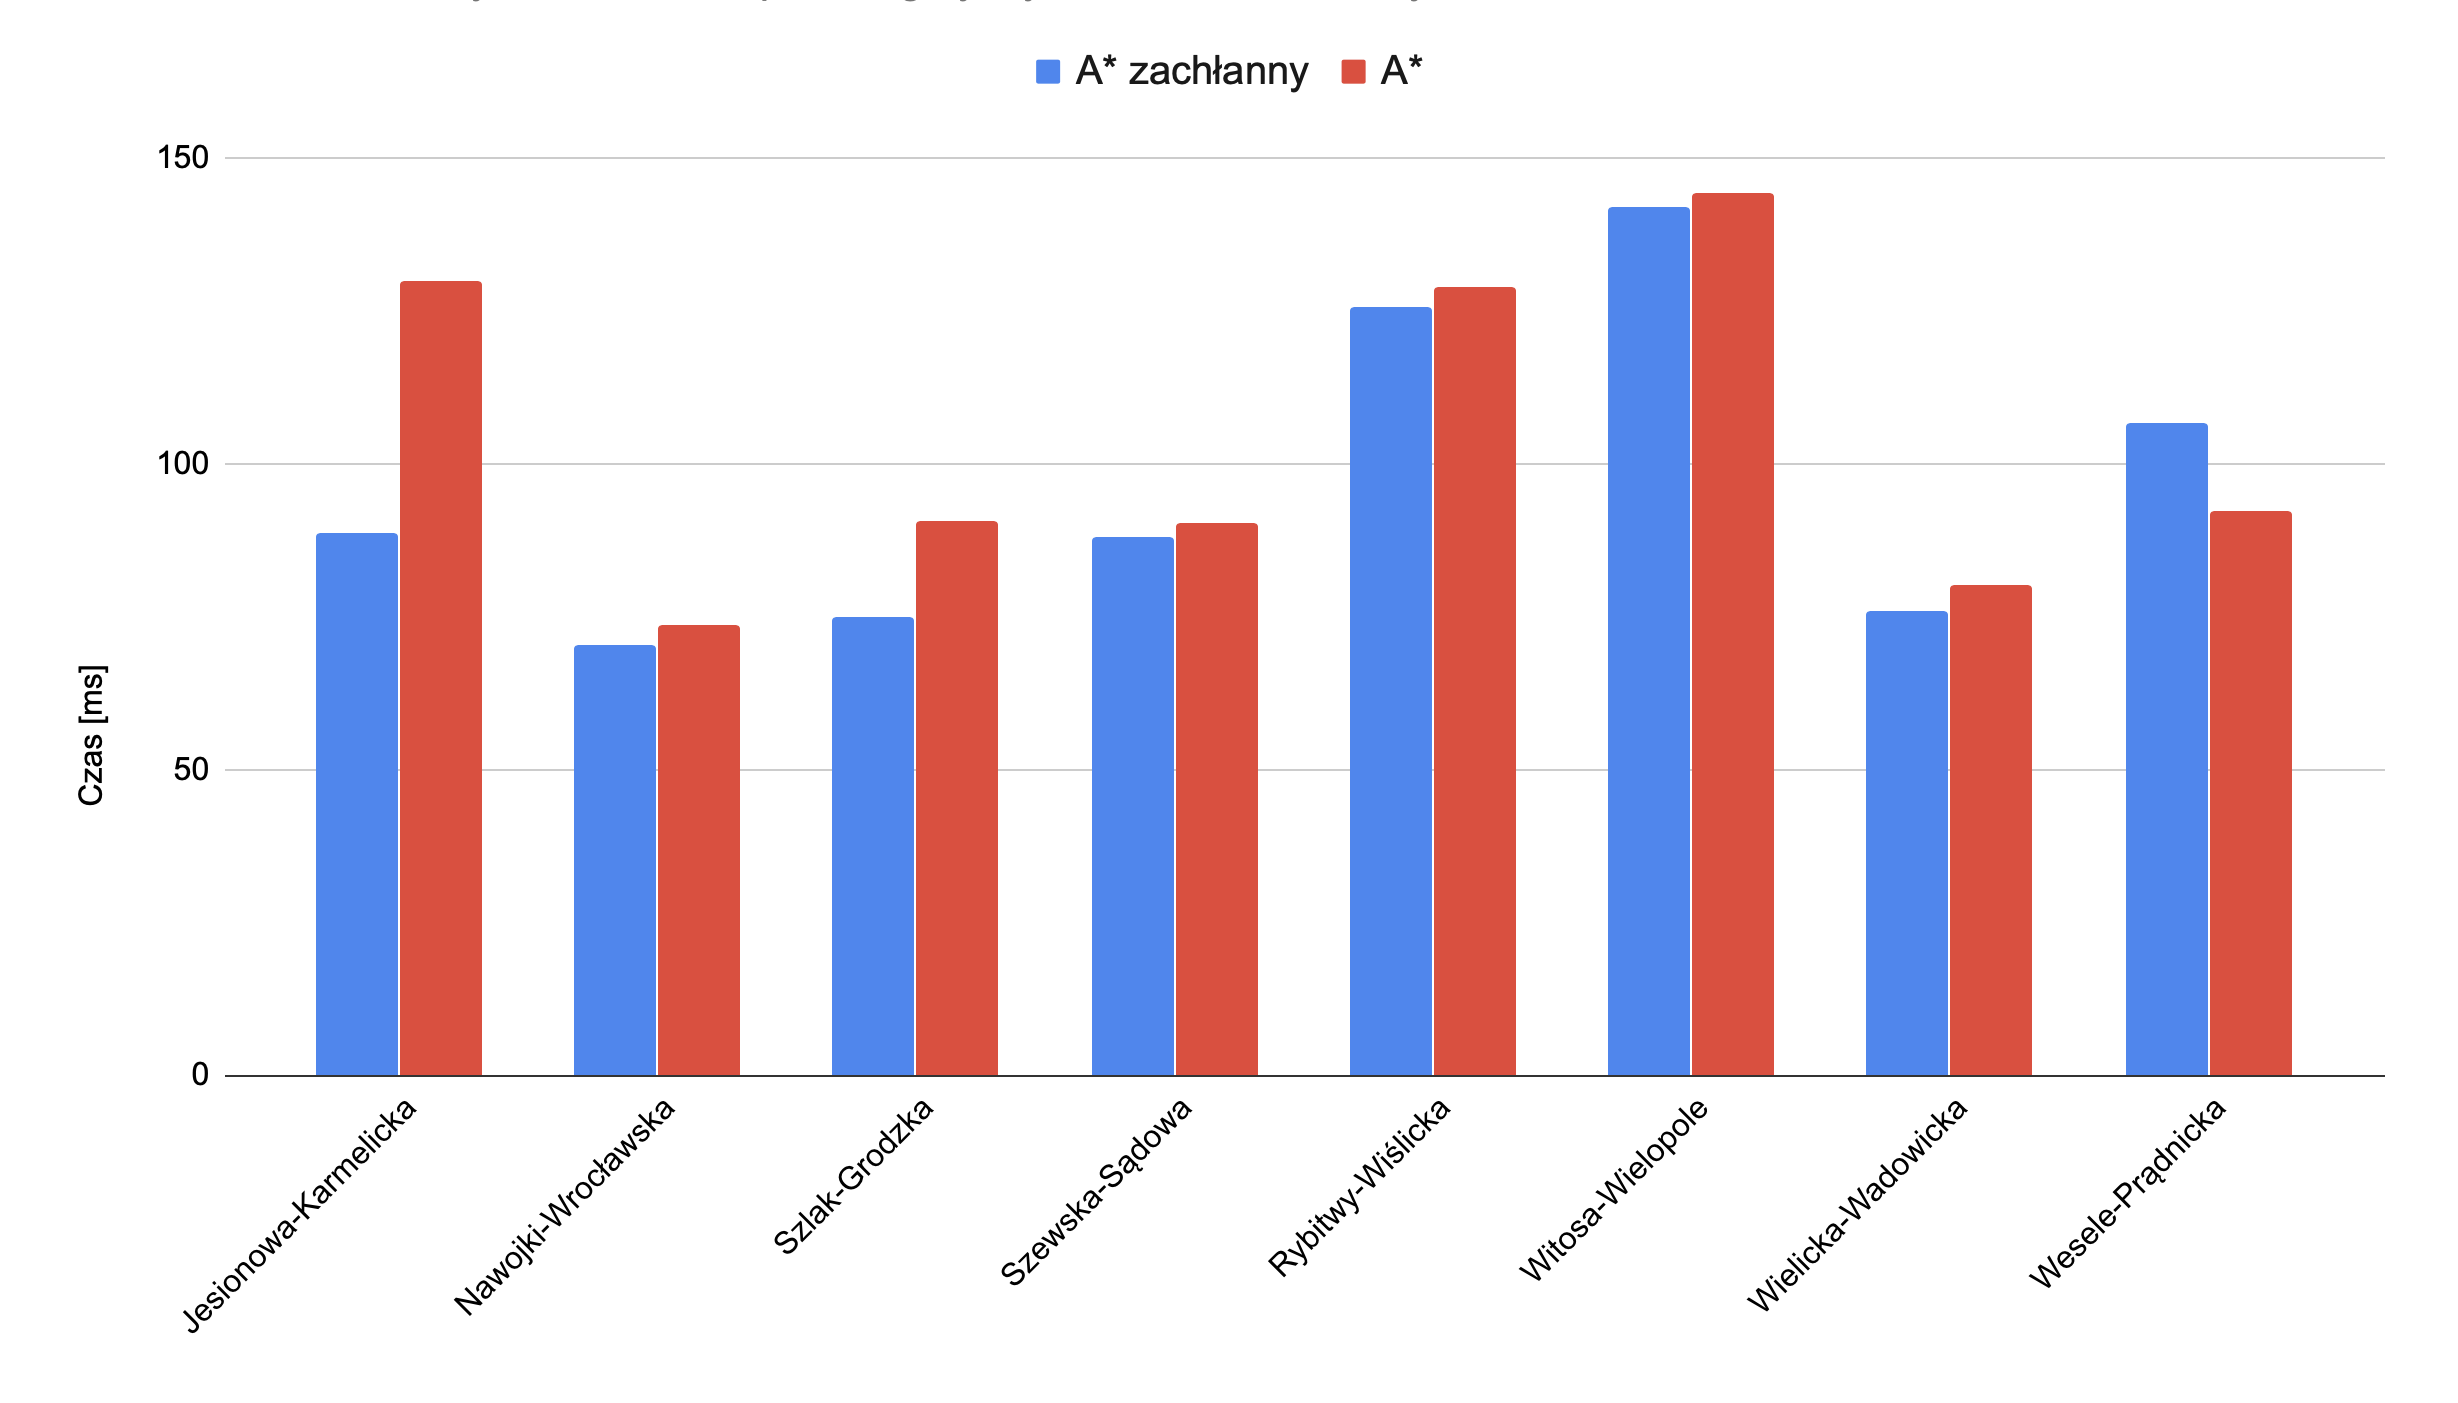
\includegraphics[width=0.7\textwidth]{czas_a_vs_a_greedy}
\caption{Zestawienie czasów wykonania algorytmów A* oraz A* zachłannego dla wybranego zestawu danych testowych.}
\end{figure}

Za wyjątkiem jednego przypadku, który może być spowodowany chwilową mniejszą wydajnością maszyny na której działały testy, algorytm zachłanny uzyskał lepszy średni czas wyznaczania trasy. Jest to spodziewany rezultat, ponieważ algorytm ten w swojej zasadzie działania stara się optymalizować czas wykonania kosztem jakości. Różnice w czasie działania dla większości przypadków są bardzo niewielkie, sumując je z brakiem gwarancji wyznaczenia trasy optymalnej, algorytm zachłanny A* nie znajduje zastosowania w stworzonym algorytmie.

\subsection{Porównanie algorytmu NBA i standardowej implementacji A*}

W celu dalszej analizy możliwych usprawnień dla czasu działania algorytmu, został zaimplementowany i porównany także algorytm NBA*(\textit{New Bidirectional A*}). Jest to odmiana algorytmu A*, który w celu optymalizacji czasu działania jednocześnie rozpoczyna swoje wykonywanie z punktu końcowego do punktu początkowego oraz w przeciwną stronę. Złożoność obliczeniowa wykonania obydwu algorytmów pozostaje taka sama, jednak istnieje możliwość wykonywania dwóch algorytmów przy wykorzystaniu dwóch rdzeni procesora, dzięki czemu czas obliczeń ulega znacznej poprawie. W przeciwieństwie do algorytmu zachłannego, algorytm NBA gwarantuje każdorazowe wyszukanie optymalnej trasy w grafie.

Na poniższym wykresie przedstawiono zestawienie czasów działania algorytmów. W celu otrzymania porównywalnych wyników, porównania zostały także przeprowadzone dla tego samego zestawu danych testowych.

\begin{figure}[H]
\centering
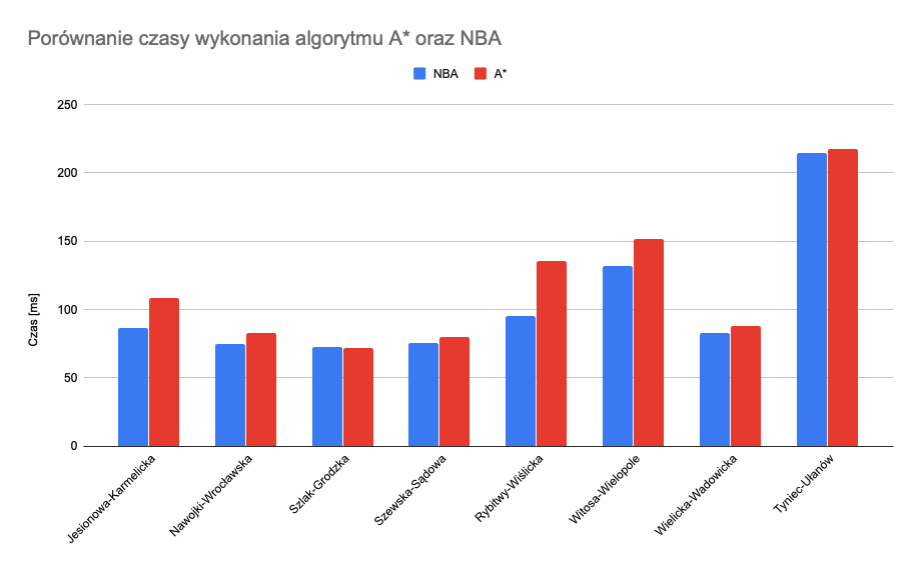
\includegraphics[width=0.7\textwidth]{czas_a_vs_nba}
\caption{Zestawienie czasu wykonania algorytmu A* oraz NBA dla wybranego zestawu danych testowych.}
\end{figure}

Z otrzymanych wyników można odczytać, że algorytm NBA daje możliwość uzyskania nieznacznie mniejszych czasów obliczeń. Same różnice nie są duże, ale znikomym nakładem pozwalają nieznacznie obniżyć wykorzystanie zasobów serwera w przypadku, gdy aplikacja jest używana przez sporą ilość ludzi. Z wykresu można także odczytać nieznaczny trend w kierunku zwiększenia różnic czasów wykonania algorytmu w przypadku, gdy trasy są dłuższe. Jest to spowodowane faktem, że zasoby czasowe potrzebne na alokację oraz rozpoczęcie procedury przeszukiwania grafu z obydwu stron mogą być skompensowane przez rzeczywisty zysk uzyskany przez samą procedurę przeszukiwania. Czas obliczeń dla tras o długości 800-2000m jest w przypadku obydwu algorytmów prawie taki sam.

\subsection{Przeprowadzenie testu użycia procesora dla aplikacji serwerowej w zależności od zastosowania algorytmu A* lub NBA}

Korzystając z wiedzy odnośnie czasu wykonywania oraz jakości analizowanych algorytmów, zostały wybrane dwa z nich, które gwarantują wyszukanie optymalnej ścieżki w grafie. Nie tylko bliskiej rozwiązaniu optymalnemu, jak w przypadku A* zachłannego. Wybrane algorytmy gwarantują czas wykonywania umożliwiający swobodne działanie aplikacji w środowisku produkcyjnym. W tym kroku został także odrzucony algorytm Dijkstra, jako że czas jego wykonania uniemożliwiał swobodne korzystanie z aplikacji przez użytkowników. Dla wybranych algorytmów, A* i NBA, zostały przeprowadzone testy które miały na celu pomiar użycia mikroprocesora podczas wykonywanych przez komputer obliczeń. Do pomiaru aktualnego użycia procesora została użyta wbudowana aplikacja ps, wyniki zostały przedstawione na poniższych wykresach.

\begin{figure}[H]
\centering
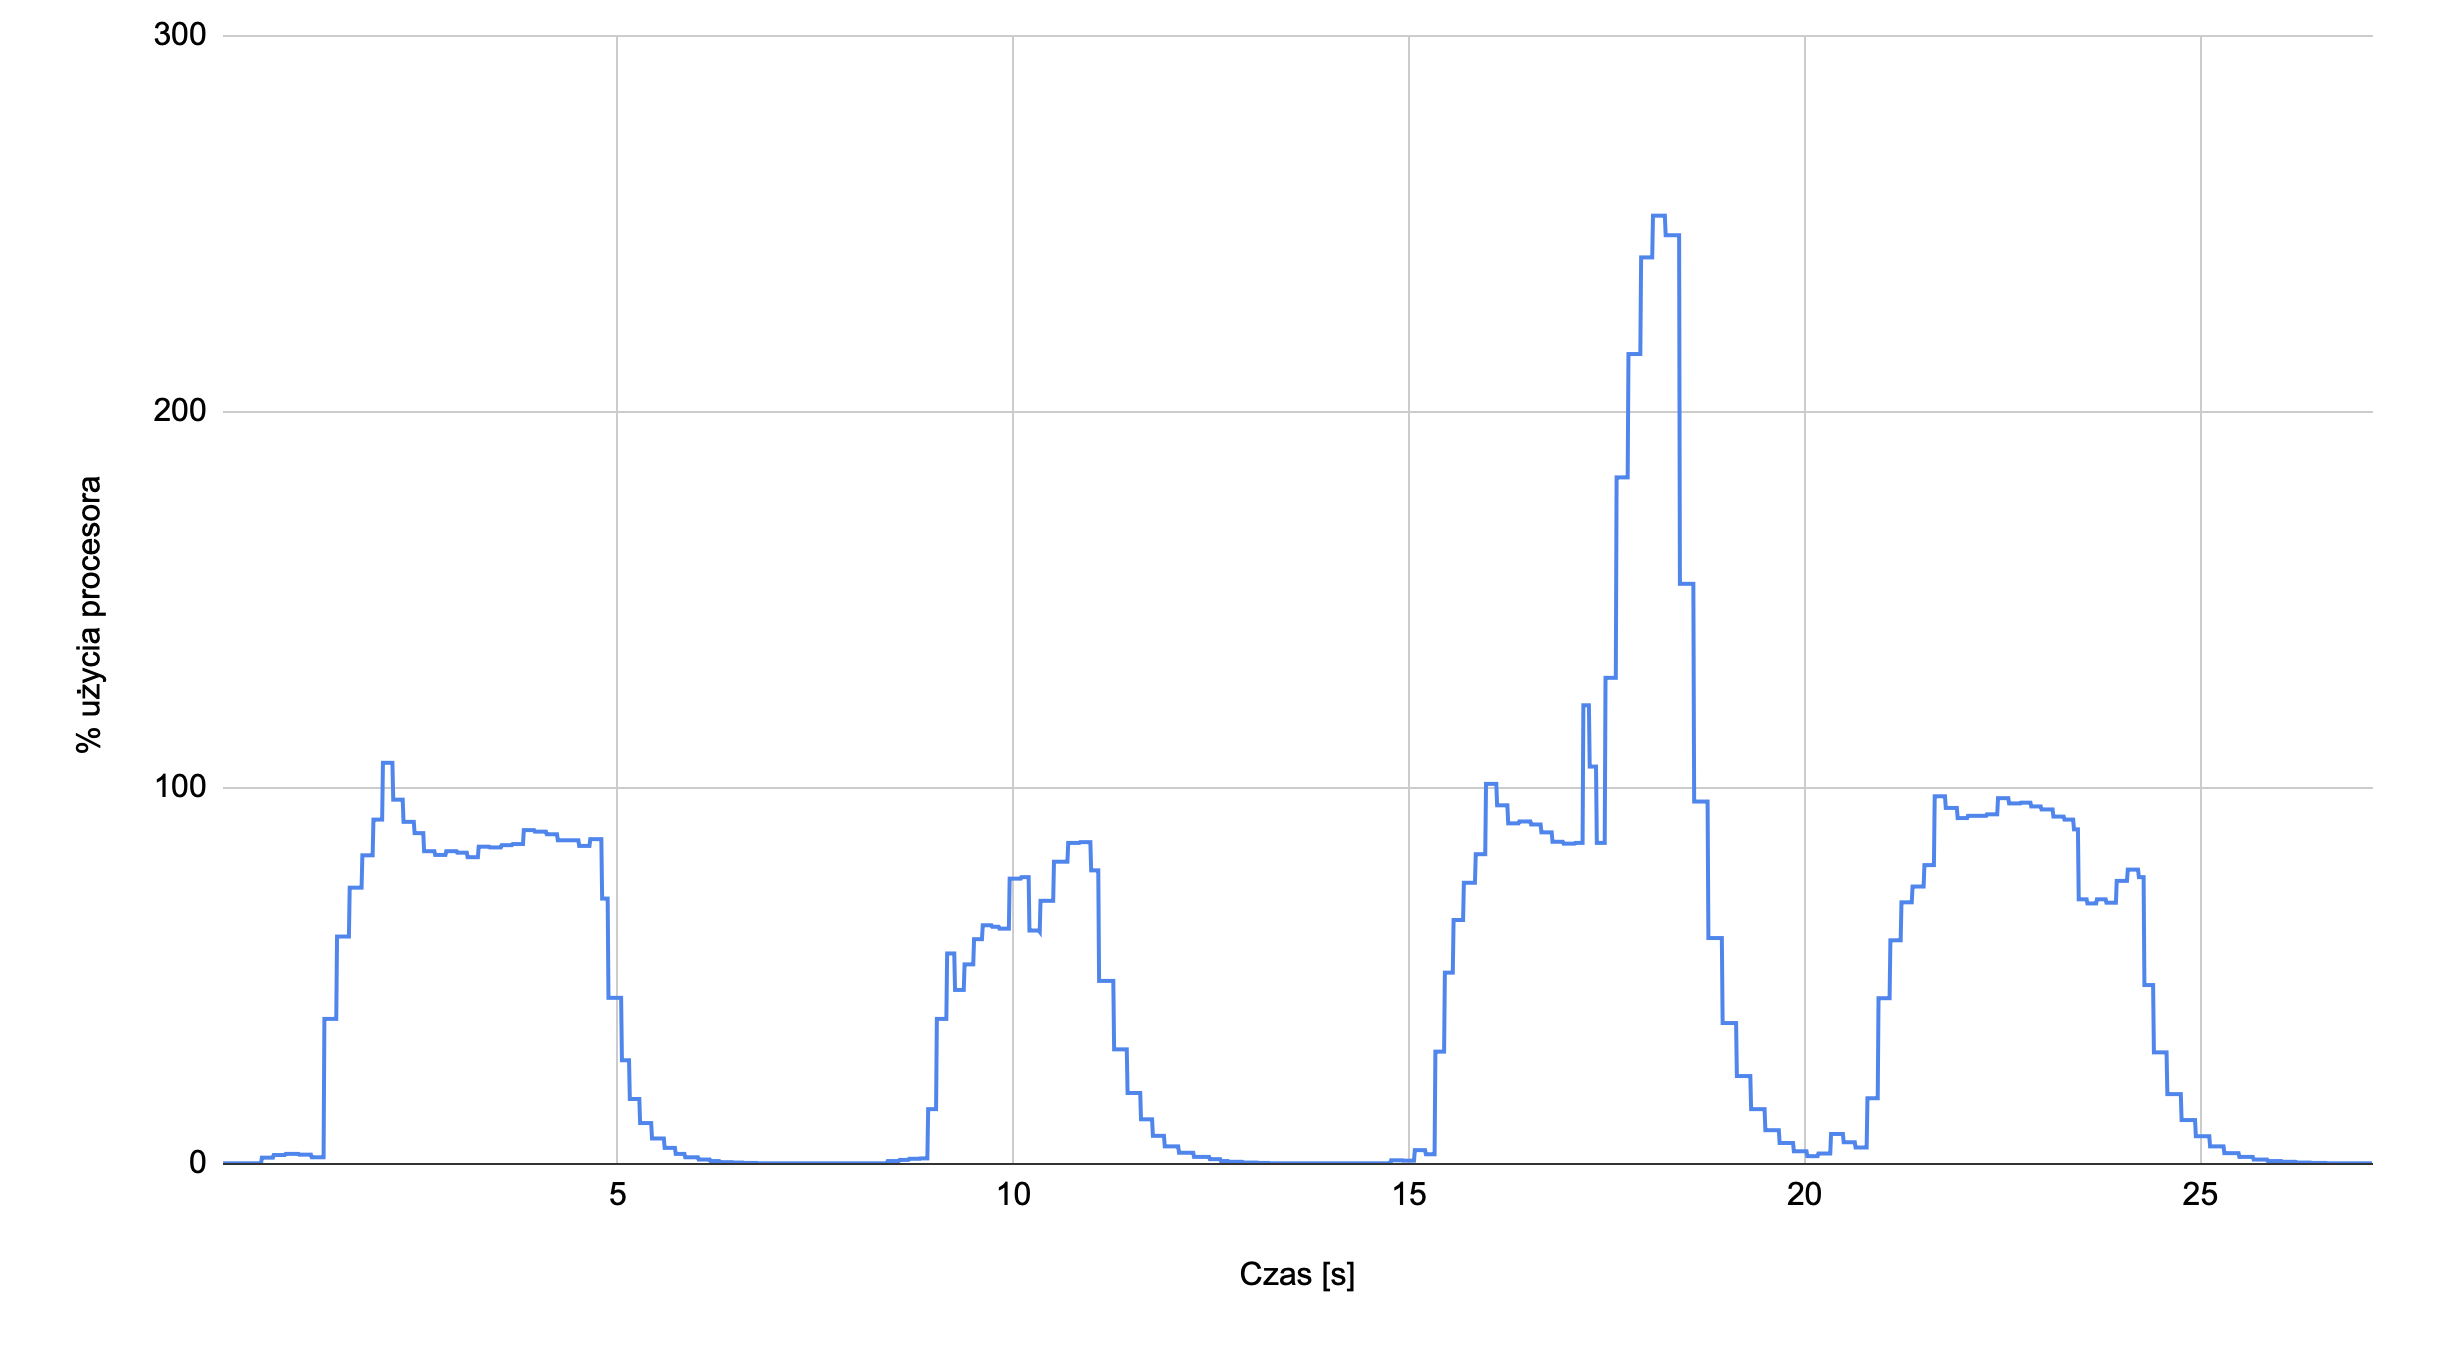
\includegraphics[width=0.7\textwidth]{a_star_cpu}
\caption{Wykres procentowego użycia procesora przy wykonywaniu algorytmu A*.}
\end{figure}

\begin{figure}[H]
\centering
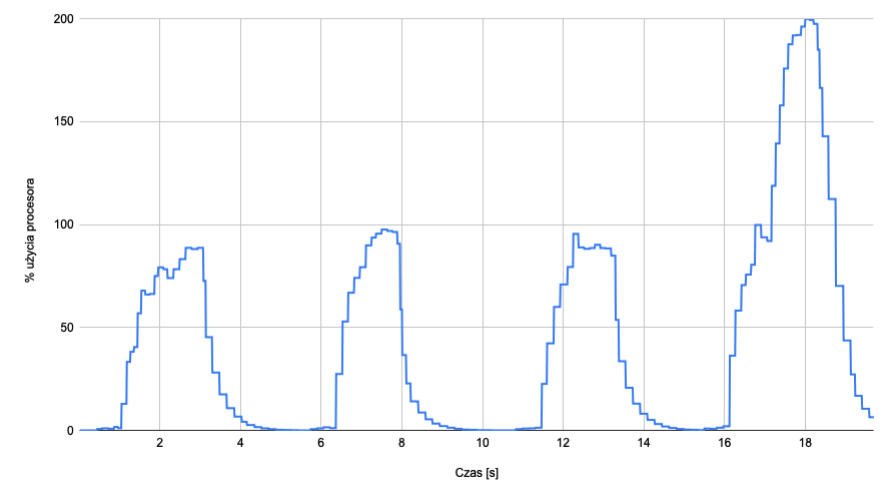
\includegraphics[width=0.7\textwidth]{nba_cpu}
\caption{Wykres procentowego użycia procesora przy wykonywaniu algorytmu NBA.}
\end{figure}

Na przedstawionych wykresach każda ze szpilek oznacza pojedyncze wykonanie zapytania do serwera, więc także obliczenie algorytmu. Test ma na celu sprawdzenie czy obydwa użyte algorytmu podczas swojego działania używają maksymalnych zasobów mikroprocesora maszyny na której są włączane. Z wykresów można odczytać że algorytmy wykazują podobne użycie procesora. Szpilki wychodzące powyżej dwustu lub nawet trzystu procent są związane z dodatkowymi procesami włączanymi przez środowisko Node podczas wykonywania zapytań a wyjście powyżej stu procent użycia procesora oznacza użycie wielu rdzeni jednocześnie.

\section{Porównanie wyników w stosunku do tras wyznaczonych przez Google Maps}

W celu przedstawienia rzeczywistego kontekstu dla przeprowadzanych pomiarów, w ostatnim punkcie porównania dokonano analizy tras wyznaczanych przez stworzoną aplikację w stosunku do tych wyznaczanych przez najbardziej popularną wyszukiwarkę tras zarówno samochodowych, rowerowych, jak i pieszych oferowaną przez Google Maps. Na poniższym wykresie przedstawiono zestawienie długości wyznaczonych tras w zależności od wybranej opcji trasy, najkrótszą lub najlepszą, z odpowiadającą temu trasą Google.

\begin{figure}[H]
\centering
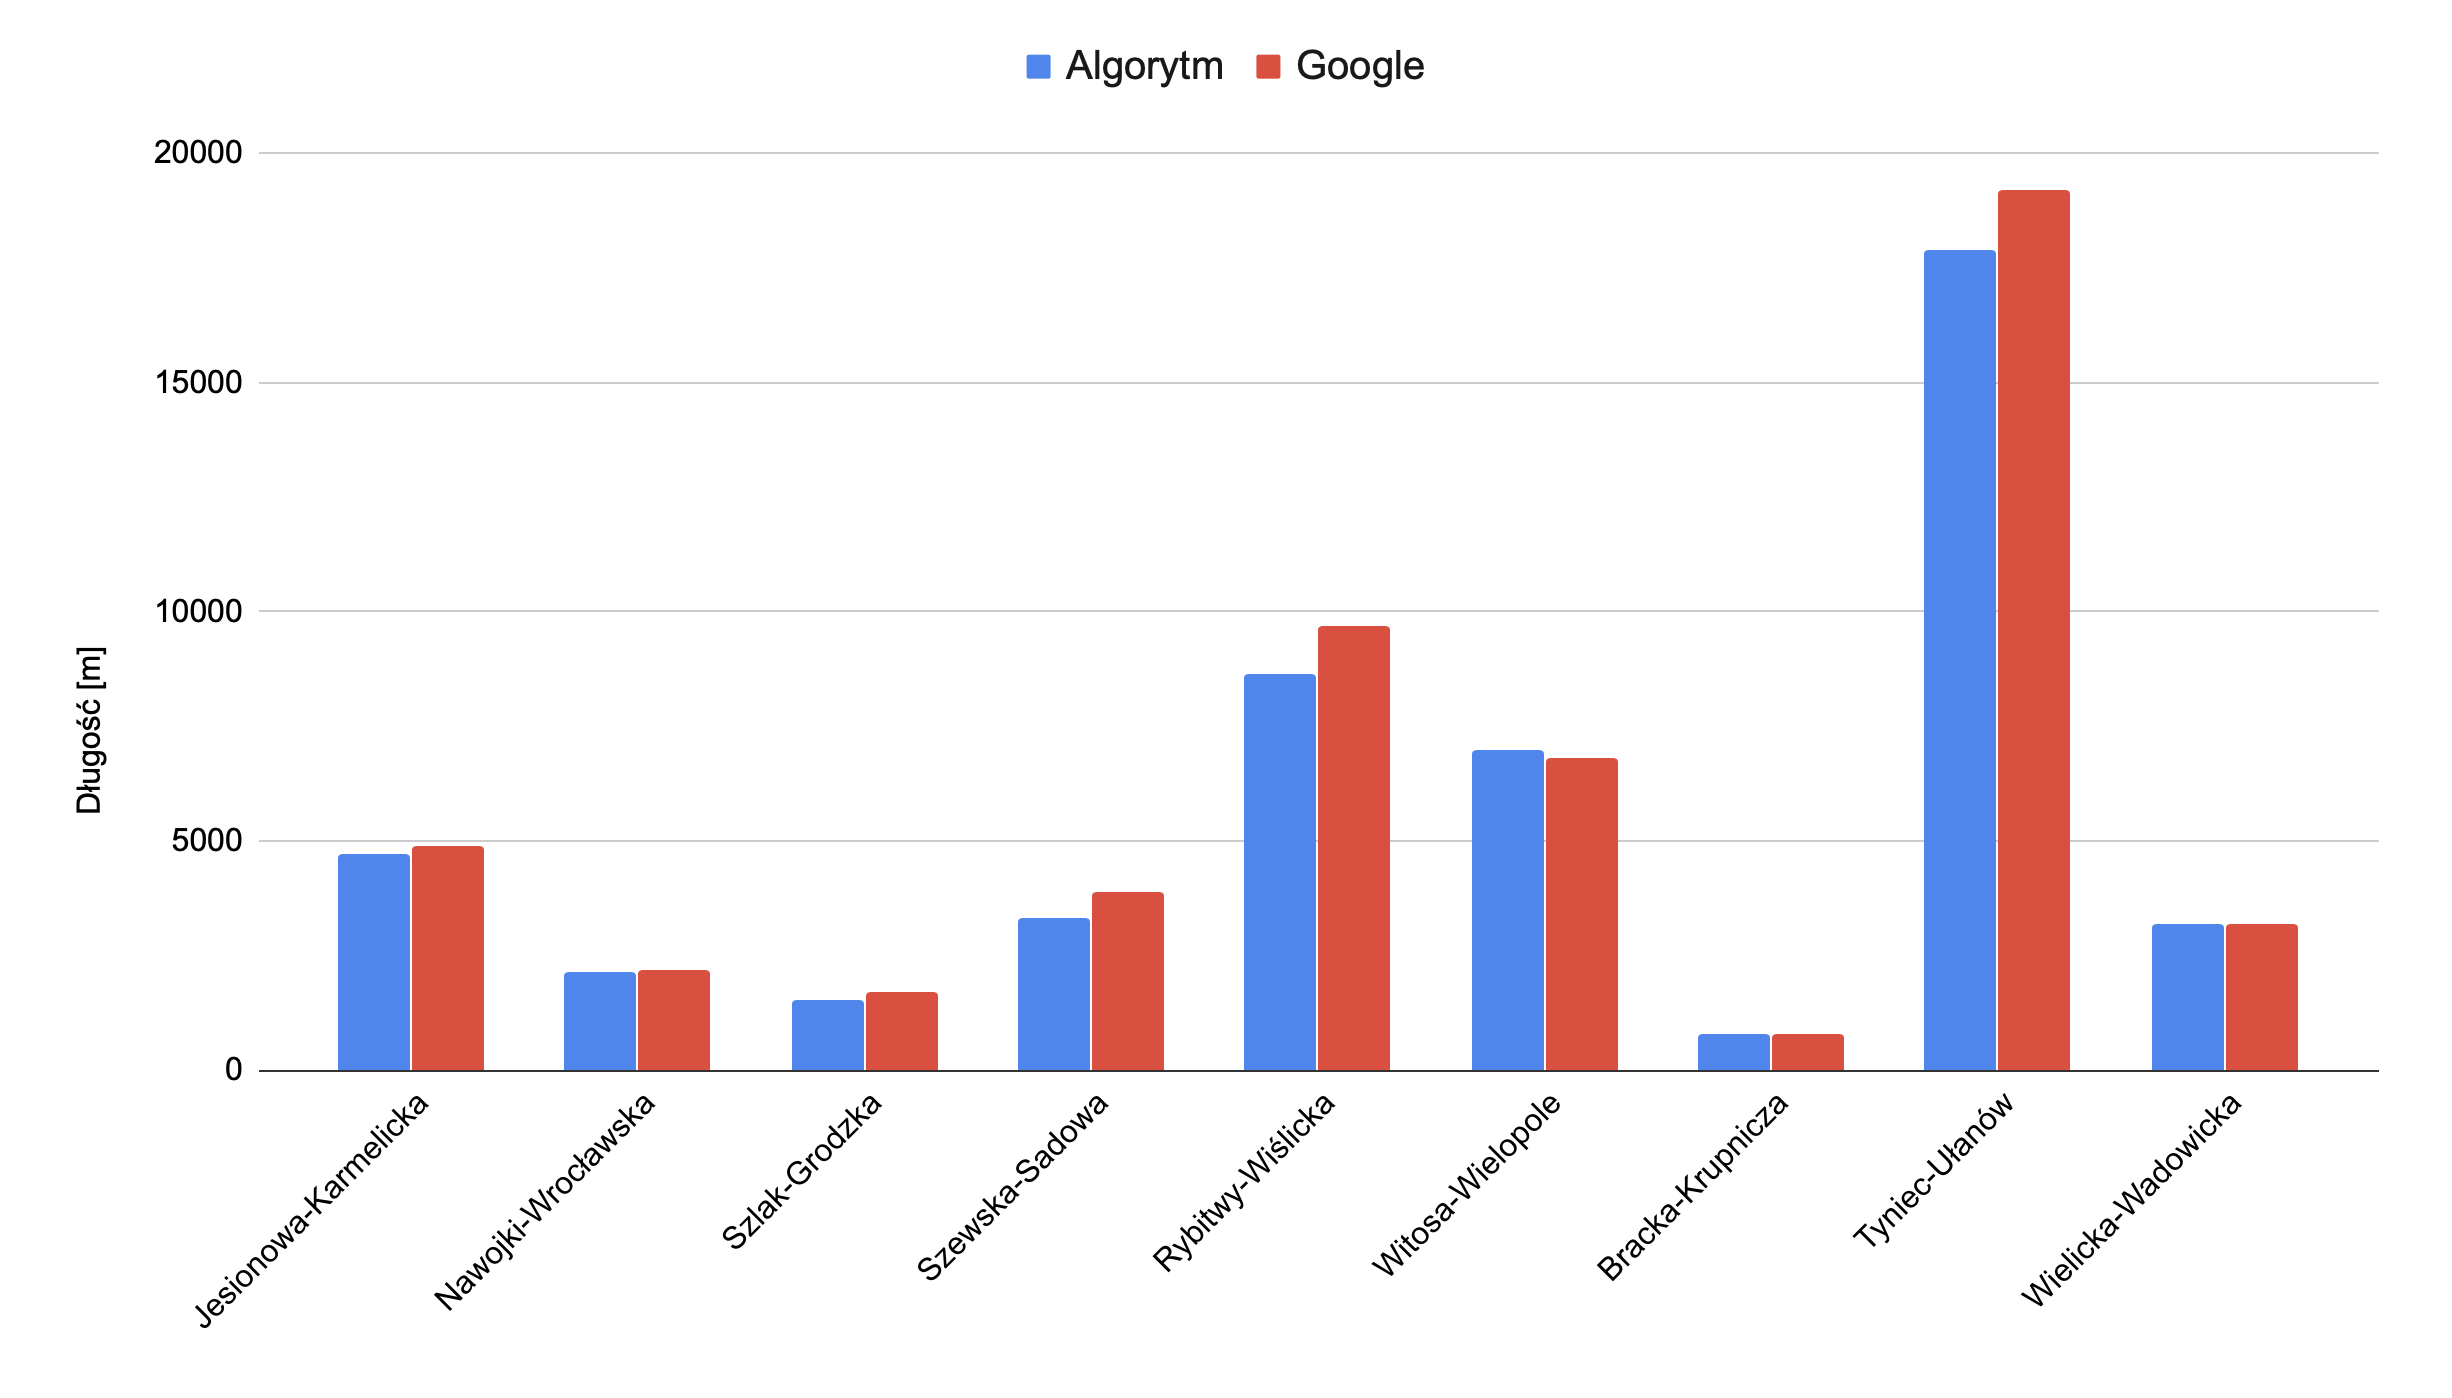
\includegraphics[width=0.7\textwidth]{google_vs_algo_najkrotsza}
\caption{Porównanie długości tras wyznaczonych przez aplikację oraz Google Map przy wyborze najkrótszej trasy.}
\end{figure}

\begin{figure}[H]
\centering
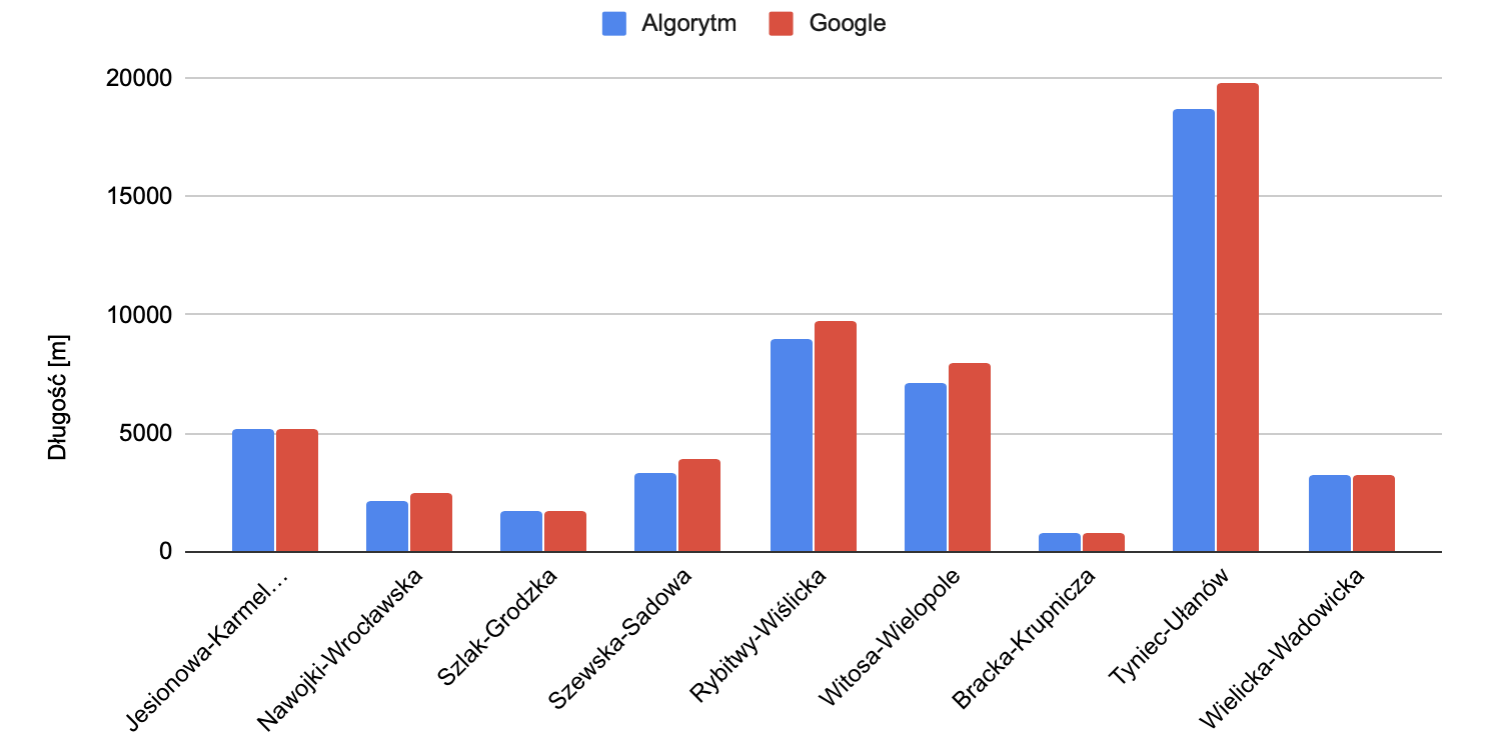
\includegraphics[width=0.7\textwidth]{google_vs_algo_najlepsza}
\caption{Porównanie długości tras wyznaczonych przez aplikację oraz Google Map przy wyborze najlepszej trasy.}
\end{figure}

Z powyższych porównań można odczytać, że w większości przypadków, zaproponowany algorytm wyznaczył trasy krótsze niż wyszukiwarka Google. W przypadku nieznacznych różnic może to być spowodowane przez różne poprowadzenie punktów na mapie składających się na drogi, można jednak znaleźć 3 przypadki, w których trasy zostały poprowadzone inaczej i skutkowało to ich skróceniem. Dodatkowym zyskiem podczas korzystania z zaproponowanego rozwiązania jest pewność, że użytkownik zostanie poprowadzony przez drogi dla rowerów lub miejsca umożliwiające swobodne poruszanie się na rowerze. W przypadku map Google trasa wyznaczana jest także po ulicach bez zmniejszonych ograniczeń prędkości. Niestety dostęp do algorytmu wyznaczania tras przez aplikację Google jest zamknięty, nie jesteśmy w stanie bezpośrednio porównać działania obydwu algorytmów, możemy jednak na podstawie obserwacji przewidywać. Różnica w działaniu, działająca na korzyść  rozwiązania będącego przedmiotem tej pracy, jest spowodowana głównie brakiem odpowiednich danych odnośnie dróg typu kontrapas poprowadzonych w przeciwnym kierunku w stosunku do jednokierunkowych ulic dla samochodów.
\chapter{Wnioski i możliwe dalsze usprawnienia}
\label{cha:wnioski}

Podczas tworzenia rozwiązania zaproponowanego jako część powyższej pracy, napotkano mnóstwo przeszkód oraz przypadków brzegowych w których algorytm nie funkcjonował poprawnie. Większość tych przypadków była spowodowana brakiem kontekstu geograficznego przy łączeniu punktów na mapie podczas poszukiwania przyległości wierzchołków w procesie tworzenia grafu używanego przy wyszukiwaniu optymalnych tras. Przy założeniu wyszukiwania przyległości w odległości 30 metrów, algorytm nie był w stanie stwierdzić czy pomiędzy punktami nie znajduje się naturalna przeszkoda jak na przykład płot lub ciek wodny. Także poza prostym przewidywaniem nie jest w stanie stwierdzić, czy łączone wierzchołki znajdują się na tej samej wysokości lub nie ma pomiędzy nimi przepaści, tutaj za przykład można podać wykrywanie skrzyżowań pomiędzy trasą znajdującą się na moście oraz drogą przebiegającą pod nim. Dodatkowym problemem był także brak pewności co do poprawności wag przyznawanych każdej z dróg w procesie tworzenia grafu. Dane te były dobierane na podstawie eksperymentów i wielu iteracji testów przeprowadzonych podczas tworzenia rozwiązania. \newline
Jedynym sposobem na pewność że trasy są poprawnie ze sobą połączone oraz mają poprawnie przypisane wagi jest stworzenie narzędzia do ręcznego wprowadzania tras oraz łączenia ich pomiędzy sobą wierzchołkami. Proponowane narzędzie będzie jednocześnie prezentowało wszystkie oznaczenia w czasie rzeczywistym zaznaczone na mapie. W ten sposób, dodając do procesu prosty sposób edycji wprowadzonych danych dla przypadków brzegowych oraz wykluczając maszynowe tworzenie wierzchołków, można uzyskać pewność, że użytkownik zostanie w każdym przypadku poprawnie poprowadzony po trasie. W analizowanym zbiorze danych geo-przestrzennych znajduje się 1040 dróg, przeniesienie ich przez człowieka przy użyciu stworzonego dedykowanego rozwiązania nie powinno być czasochłonne. \newline
Dodatkowym zyskiem z zastosowania opisanego wcześniej usprawnienia jest możliwość nadania użytkownikom prawa do samodzielnej edycji danych znajdujących się w grafie. Wymaganie to jest spowodowane bardzo rzadką aktualizacją danych przez miasto Kraków w portalu zikit.carto.com. W momencie pisania pracy, ostatnia aktualizacja zbioru dróg rowerowych miała miejsce w lipcu roku 2018 co niesie za sobą konsekwencje braku wielu tras istniejących już na mapie miasta Kraków. Jednym z dalszych proponowanych usprawnień działania projektu jest także dodanie strony umożliwiającej wprowadzanie przez użytkowników nowych tras, połączonych z istniejącą infrastrukturą, które mogą być akceptowane i dołączane do zbioru tras w grafie przez zarządcę systemu z poziomu panelu administracyjnego. \newline
Z punktu widzenia analizy zastosowanych algorytmów trasowania, rozwiązaniami bliskimi optymalnemu są zarówno algorytmy A* jaki NBA, reszta analizowanych algorytmów nie gwarantowała optymalnego rozwiązania, co jest w przypadku analizowanego systemu parametrem kluczowym, lub działała zdecydowanie zbyt wolno aby mieć realne zastosowanie. Obydwa wymienione algorytmy gwarantują czas przeszukiwania grafu w celu znalezienia najkrótszej ścieżki w czasie który nie obciąża zbytnio serwera i jest komfortowy dla użytkownika w kontekście czasu ładowania się strony internetowej. Różnice w zastosowaniu obydwu wymienionych algorytmów mają znaczenie tylko w zastosowaniu globalnym, gdy z zaproponowanej aplikacji serwerowej będzie korzystać znaczna ilość użytkowników. W takim wypadku zmniejszenie kosztów utrzymania infrastruktury nawet o kilka procent gwarantuje znaczne zyski. W przypadku analizy algorytmów dla dużej skali działania oprogramowania, lepszym rozwiązaniem wydaje się być algorytm NBA. Algorytm ten gwarantuje nieznaczną poprawę w czasie działania nie alokując dodatkowych zasobów systemowych w porównaniu z algorytmem A*. Dla aktualnej skali rozwiązania zaproponowanego w powyższym opracowaniu, algorytmy są sobie równe.



% itd.
% \appendix
% \include{dodatekA}
% \include{dodatekB}
% itd.

\printbibliography

\end{document}
